% LREC 2026 Example; 
% LREC Is now using templates similar to the ACL ones. 
\documentclass[10pt, a4paper]{article}

% custom commands
\usepackage{xcolor}
\usepackage{colortbl}
\usepackage{expex}
\usepackage{tikz}
\usepackage{pgfplots}
\pgfplotsset{compat=1.18}
\usepackage{longtable}
\usepackage{booktabs}
\usepackage{amsmath}
%\usepackage{tikz-dependency}
\newcommand{\pg}[1]{{\color{blue}#1}}
\newcommand{\sy}[1]{{\color{red}#1}}
\newcommand{\drafttext}[1]{{\color{gray}#1}}
\newcommand{\corpus}[1]{{\color{gray}#1}}

% MAL mini-plot colours
\definecolor{malgreen}{HTML}{27ae60}
\definecolor{malred}{HTML}{e74c3c}
\definecolor{malgray}{HTML}{f39c12}
\definecolor{malblue}{HTML}{3498db}


% -----------------------------------

\usepackage{lrec2026} % this is the new style
% the 'review' option anonymizes the paper following submission guideline
% the 'final' option produces the camera ready version (non anonymized)
% default version is 'final', so use review option for submission

\title{Verifying the Menzerath-Altmann Law\\ in the Verbal Domain in 180 Languages}


\name{Pegah Faghiri\textsuperscript{1,2}, Kim Gerdes\textsuperscript{2}, Sylvain Kahane\textsuperscript{1,3}\thanks{Authors are listed in alphabetical order.}} 

\address{\textsuperscript{1}Paris Nanterre University, Modyco, CNRS~~
\textsuperscript{2}Paris-Saclay University, LISN, CNRS\\
\textsuperscript{3}IUF - Institut Universitaire de France \\
pfaghiri@parisnanterre.fr, kim.gerdes@universite-paris-saclay.fr, skahane@parisnanterre.fr\\}


\abstract{We present a large-scale evaluation of the Menzerath-Altmann law (MAL) in the verbal domain across 180 languages, using the Universal Dependencies (UD) treebank collection (v2.17). MAL predicts that as the number of constituents of a linguistic unit increases, their average size decreases. We propose a metric to estimate the MAL effect across corpora of widely varying sizes and define threshold-based categories to classify languages along a MAL preference cline. Crucially, we analyse the preverbal and postverbal domains separately, in addition to the standard bilateral MAL, and control for potential sampling bias by comparing results across language families (Indo-European vs.\ non-Indo-European) and syntactic types (VO, OV and no dominant order). Our results confirm MAL as a typologically widespread preference but not an absolute universal: several languages display a trivial or even opposite (anti-MAL) tendency. Furthermore, we uncover a significant asymmetry between the two sides of the verb: the MAL effect is stronger in the postverbal domain, while anti-MAL is stronger in the preverbal domain. VO languages tend to show a stronger MAL preference postverbally, whereas OV languages do so preverbally. These findings challenge the widespread assumption that length-based ordering constraints apply symmetrically on both sides of the verb and contribute new cross-linguistic evidence to the debate on the interaction between dependency length minimization and constituent size.
 \\ \newline \Keywords{Menzerath-Altmann law, quantitative typology, Universal Dependencies, verbal valency, constituent length, word order} }

\begin{document}

\maketitleabstract

\section{Introduction}

The current version of the Universal Dependencies (UD) collections of syntactic treebanks allows us to  evaluate (a number of)  universal properties on a set of 180 languages \citep{demarneffe2021universal}. In this paper, we study the (typological) validity of  the so-called Menzerath-Altman law (MAL) on the nature of complexity in linguistic units in terms of the relationship between the size of a given unit and the size of its components in any given domain \citep{menzerath1928einige, menzerath1954architektonik, altmann1980prolegomena}. Roughly speaking, the bigger the number of components of a given unit, the smaller their respective length. In the verbal domain, for instance, this implies that the length of verbal arguments decreases as the valency or number of verbal dependents increases \citep{macutek2017menzerath}. Our aim is also to propose a reliable metric to evaluate this hypothesis in the (unbalanced) UD collection with annotated corpora of significantly different sizes - including the so-called LOL languages, with millions of tokens, but also a number of corpora from less-studied languages with less than a thousand tokens. Furthermore, in order to be able to make typologically relevant claims based on an ad hoc language sample which is not construed for such purposes in the first place, we compare a number of typologically valid subsets of our sample to ensure that our conclusions are replicable beyond the sample as a whole and are not mere artefacts of sampling bias. Another important contribution of our study is that we looked at preverbal and postverbal domains separately. That is, we calculated two additional sets of metrics in addition to our general (or combined) MAL metrics, respectively LMAL and RMAL (for left/preverbal and right/postverbal arguments). 
Our results show that MAL is a clear typologically wide-spread preference across the languages of the world, but it is not an absolute universal principle. Importantly, we find that while MAL is a strong statistical cross-linguistic preference, there are not only languages in which this preference is trivial, but also languages which display the opposite tendency.  Furthermore, our results show a clear difference between the pre- and postverbal domains. On the one hand, the MAL preference is stronger in the postverbal domain and, on the other hand, the anti MAL preference is stronger in the preverbal domain. Importantly, our findings show that in the postverbal domain VO languages are more likely to show a strong RMAL preference and inversely OV languages are more likely to show a strong LMAL preference in the preverbal domain. 

In the following, we first briefly present MAL and the previous studies on which we are building (Section \ref{MAL}). We next present our data extraction based on the UD annotation (Section \ref{UD}) and the different metrics we use in this study and motivate our methodological choices (Section \ref{metrics}). We then present our results and discuss our findings (Section \ref{results}).
\section{The Menzerath-Altman law in the verbal domain}\label{MAL}
MAL predicts a negative correlation between constituents’ average length and their total number in any given domain. MAL has been previously studied in the verbal domain using the UD annotation schema in  Czech \citep{macutek2017menzerath}, as well as  in the 2.3 version of the UD collection with 76 languages \citep{tanaka2021menzerath}.  
Our study builds on the latter while proposing a number of substantial improvements in order to be able to draw more reliable and typologically valid conclusions. First, we study MAL in the preverbal and postverbal domains sepertayly, in addition to the bilateral MAL. Second, our data extraction is more fine-grained than in Tanaka-Ishii’s study (see Section \ref{UD}). Third, we use the latest version of the UD, with 180 languages, offers a more important diversity of languages around the world. Finally, we analyse the data while taking into account language families as well as language types, that is, VO, OV or no dominant order (NDO).

%proposes substantial differences with Tanaka-Ishii’s study:
%\begin{itemize}
    %\item we filter verbal dependents the verbal constructions to retain only syntactic dependents and to eliminate coordinated conjuncts or discourse markers;
    %\item we also estimate the mean size of constituents on the right or on the left to see whether MAL is still verified on the half construction; 
    %\item we extend this research  by studying the 2.17 version of the UD collection which, with 180 languages, offers a more important diversity of languages around the world; 
    %\item we also have a discussion on the choice of the right metrics.
%\end{itemize}



\section{Extracting the constituents of verbal constructions in UD}\label{UD}

We assume a certain familiarity with the UD annotation scheme in this paper and simply recall that the syntactic structure of all sentences is encoded as a dependency tree. Here we focus on verbal constructions, that is, a verb and all the constituents that depend on it. We consider all lexical verbs and have decided not to restrict our study to main verbs (see (\ref{ex:notmain})) for at least two reasons: first, including all lexical verbs can double or triple the number of constructions, which is not negligible when the corpus is small; second, in some sentences, the most interesting verb in terms of construction may be subordinated because the main verb is merely a modal or an auxiliary.

All dependents of a verb (in the tree) cannot be considered constituents (of the verbal construction we are interested in). The following are excluded in our data extraction: punctuation signs (attached by the \texttt{punct} relation in UD), discourse markers (\texttt{discourse} relation; see \textit{alas} in (\ref{ex:aux})), juxtaposed clauses or parentheses (\texttt{parataxis} relation), conjuncts in a coordination (\texttt{conj} relation; (\ref{ex:coord})), and coordinating conjunctions (\texttt{cc} relation; see \textit{but} in (\ref{ex:aux})). The \texttt{vocative} relation, which concerns addresses to a participant (\textit{Guys, take it easy!}), is excluded but dislocated arguments (\textit{These guys, I don't trust them.}) are kept in, especially because in some languages the boundary between governed units and dislocated units is difficult to draw. The \texttt{aux} relation (see \textit{do} in (\ref{ex:aux})), is excluded, considering that auxiliaries are part of the verb form; compounds (see \textit{out} in (\ref{ex:out})) are excluded as well. Markers of subordination such as subordinating conjunctions and adpositions (\texttt{mark} and \texttt{case} relations; see \textit{when} in (\ref{ex:notmain})), which are analysed as dependents in UD but are generally considered as heads of their constructions, are also discarded.\footnote{In her study, \citet{tanaka2021menzerath} did not exclude any dependent, except the punctuation.}

Examples of English verbal constructions are given in (\ref{ex:1}) for illustration; the verb is underlined and the constituents are shown between square brackets; filtered elements are given in italics.

\pex\label{ex:1}
\a\label{ex:aux}\textit{But} [I] , \textit{alas} , \textit{do} [not] \underline{know} [how to see sheep] [through the walls of boxes]. \corpus{en\_littleprince}
\a\label{ex:notmain}This means that \textit{when} [you] \underline{move} [a series or category field] [to the filter area and back], previously hidden items are again hidden. \corpus{en\_lines}
\a\label{ex:coord}[You] \underline{tell} [me] [what they look like] \textit{and I'll tell you what they are}. \corpus{en\_childes}
\a\label{ex:out}[One minister] [reportedly] \underline{handed} \textit{out} [100 dollar `gifts'] [to journalists attending a press conference for Allawi], [a practice that brings back bad memories to many Iraqis]. \corpus{en\_ewt}
\xe

Another possibility taken into account is that a constituent may be split into two contiguous parts, for example in cases of extraction or extraposition. These cases are treated as two separate constituents. For instance, in (\ref{ex:what}), the relative pronoun \textit{what} is extracted and separated from its governor \textit{do}, and in (\ref{ex:extra}), the relative clause \textit{that go well with the Santorum cocktail} is extraposed and separated from its governor \textit{dishes}.

\pex
\a\label{ex:what}[What] \textit{do} [you] \underline{like} [to do] ? \corpus{en\_ewt} 
\a\label{ex:extra}[What culinary dishes] \textit{would} [you] \underline{recommend} [that go well with the Santorum cocktail]? \corpus{en\_gum}
\xe

For each language L and each $n \geq$ 1, we extracted all the verbal constructions with $n$ constituents. We then calculated the size of each constituent, excluding punctuation. In other words, we kept all relations except \texttt{punct}; if a constituent contains a coordination or a discourse marker, there is no reason to remove them. 

We call MAL$_n$(L) the mean size of the constituents in all verbal constructions with $n$ constituents. Note that we compute MAL$_n$(L) for a given language L only when we have at least 100 constructions with $n$ constituents. We return to this point in Section~\ref{metrics}. We define LMAL$_n$(L) and RMAL$_n$(L) in the same way. For LMAL, all constructions with $n$ preverbal constituents (i.e.\ on the left) were selected, regardless of the other side of the verb. Likewise for RMAL, with all constructions having $n$ postverbal constituents (i.e.\ on the right).


\section{Defining the MAL effect in the UD collection}\label{metrics}

We call $\lambda$MAL(L) the function that mapst MAL$_n$(L) to each $n$. It has been shown by \citet{altmann1980prolegomena} that a function such as $\lambda$MAL(L) should follow a power law. In other words, MAL$_n$(L) is expected to be more or less proportional to $n^{-\beta}$ where $\beta$ is a positive value (generally smaller than 1), which we call the MAL effect for L. 
Note that if MAL$_n$(L) $\approx n^{-\beta}$, then log(MAL$_n$(L)) $\approx -\beta$log($n$). In other word, $-\beta$ is the slope of the regression line of the log-log representation of $\lambda$MAL(L). The greater is $\beta$, the quicker is the decrease, the stronger is the MAL effect. Figure \ref{fig:German} gives the value of $\beta$ (1.171) as well as the coefficient $R^2$ (0.892), which shows that $\lambda$MAL(German) is close to a power law and that MAL is verified for German.

\begin{figure}[!ht]
\begin{center}

\includegraphics[width=\columnwidth]{latex/German.png}
\caption{$\lambda$MAL(German).}
\label{fig:German}
\end{center}
\end{figure}

%There are also languages that do not clearly follow a power law. This is the case of OldEast Slavic which not only has an Anti MAL effect (the mean length of the constituents increase with the number of constituents) but on top of that the Anti MAL effect increases with the number of constituents (Figure \ref{fig:OldEastSlavic}

%\begin{figure}[!ht]
%\begin{center}
%
\includegraphics[width=\columnwidth]{latex/OldEastSlavic.png}
%\caption{$\lambda$MAL(OldEastSlavic).}
%\label{fig:OldEastSlavic}
%\end{center}
%\end{figure}

\citet{tanaka2021menzerath} showed that, on her data, the values for $n$ = 1 and $n$ = 2 may not be aligned and she took onto account only the values for $n\geq$ 3 for computing $\beta$. We think that the problem was was partly due to the fact that her data were not filtered.

We call $\beta$($j\rightarrow k$) the slope of $\lambda$MAL for $j\leq n \leq k$. If $k = j+1$, $\beta$($j\rightarrow k$) is just the slope between the point (log(MAL$_j$),log($j$)) and (log(MAL$_k$),log($k$)).
In the figure \ref{fig:1vs2}, we compare the $\beta$(1$\rightarrow$2) with $\beta$(2$\rightarrow\infty$). The important dispersion suggests that the value for MAL$_1$ is effectively poorly aligned with the other values. The case where MAL$_1$ is aligned are the point on the diagonal $y=x$.

\begin{figure*}[ht]
\begin{center}

\includegraphics[width=\textwidth]{latex/1vs2.png}
\caption{$\beta$(1$\rightarrow$2) vs $\beta$(2$\rightarrow \infty$)}
\label{fig:1vs2}
\end{center}
\end{figure*}

Nevertheless we observe that the values of MAL$_1$ can be sometimes under the regression line for $n\geq 2$ (as it is the case for German, Fig. \ref{fig:German} and sometimes above (see Czech, Fig. \ref{fig:Czech}, or Arabic, Fig. \ref{fig:Arabic}).

\begin{figure}[!ht]
\begin{center}

\includegraphics[width=\columnwidth]{latex/Arabic.png}
\caption{$\lambda$MAL(Arabic).}
\label{fig:Arabic}
\end{center}
\end{figure}

\begin{figure}[!ht]
\begin{center}

\includegraphics[width=\columnwidth]{latex/Czech.png}
\caption{$\lambda$MAL(Czech).}
\label{fig:Czech}
\end{center}
\end{figure}

We then decide to take $\beta$(1$\rightarrow\infty$) as the metric to evaluate the MAL effect. We also do that because, due to the filter and the fact that many treebanks are quite small, we do not have values of MAL$_n$ for $n\geq 4$. And it is even more problematic when we look at LMAL$_n$ and RMAL$_n$. 

 We nevertheless must mention an additional problem with $n$ = 1. While the number of configurations with $n$ constituents decrease for n $geq 2$ only 20 of the 131 languages that have at least 100 configurations for $n$ = 2 and 3 have more data $n$ = 1 than for $n$ = 2. Among them, 12 language have less that 100 configurations with one constituent ($n$ = 1) and we must take $\beta$(2$\rightarrow\infty$) to evaluate the MAL effect.
 
There are 131 languages in our sample for which we have calculated a value for $\beta$(1$\rightarrow\infty$). We identify three types of behavior in our sample and givent that our values of $\beta$(1$\rightarrow\infty$) are mainly comprised between $-0.3$ and $0.3$, we devide them into the three categories following categories:\footnote{For $\lamba$MAL, no $\beta$(1$\rightarrow\infty$) are lesser than $-0.3$ and only 9 languages have a $\beta$(1$\rightarrow\infty$) greater than $0.3$. Almost same thing for $\lamba$LMAL. For $\lamba$RMAL, 48 languages have a value greater than $0.3$!} 

\begin{itemize}
    \item Language L with $\beta$(1$\rightarrow\infty$) $\geq 0.1$ is considered to have a MAL effect;
    \item Language L with $\beta$(1$\rightarrow\infty$) $\leq -0.1$ is considered to have an Anti MAL effect.
    \item Language L with $-0.1\leq$ $\beta$(1$\rightarrow\infty$) $\leq 0.1$ is considered to be in the grey zone;
\end{itemize}

The majority of languages of our sample (that is, 62 languages which make 47\% of the 131 languages) fall into the first category, that is they show a MAL effect. But there are also a smaller number of languages (10 languages,),showing an Anti MAL effect. The remaining languages are in the gray zone (45\% of languages). 

One of the languages that do not follow a power law is OldEast Slavic, which not only has an Anti MAL effect (that is, the mean length of the constituents increase with the number of constituents), but on top of that the anti MAL effect increases with the number of constituents (Figure \ref{fig:OldEastSlavic}

\begin{figure}[!ht]
\begin{center}

\includegraphics[width=\columnwidth]{latex/OldEastSlavic.png}
\caption{$\lambda$MAL(OldEastSlavic).}
\label{fig:OldEastSlavic}
\end{center}
\end{figure}

\section{MAL compliance rate}\label{decrease}
In addition to the MAL effect, we also define a simple regression-free measure, which we call the MAL compliance ratio, which gives the proportion of paires where MAL$_n$ decrease (for instance, MAL$_n+1$ $\leq$  MAL$_n$). We calculated an average decrease ratio for MAL, LMAL and RMAL for all languages with a corresponding value for $\beta$(1$\rightarrow\infty$, and defined the three following MAL compliance types:

\begin{itemize}
    \item Language L with MAL compliance ratio $\geq 0.667$ is considered to have a high MAL compliance;
    \item Language L with MAL compliance ratio $\leq 0.334$ is considered to have a low MAL compliance.
    \item Language L with $0.334\leq$ MAL compliance ratio $\leq 0.667$ is considered to have a middle MAL complaince;
\end{itemize}

 
\section{Results}\label{results}
\subsection{MAL effect in the UD collection}\label{results1}
Out of the 186 languages available in our data, we caluclated a $\beta$(1$\rightarrow\infty$) for 131. In these sample we identify 62 languages with a MAL preference, 10 with an Anti MAL preference and 59 in the gray zone. Importantly, these three categories are fairly comparabely well-represented across languages families as well as main syntactic languge types \ref{tab:MAL}).
%For language families, given the unbalanced nature of our sample, we have grouped the languages into the two main Indo-European (IE) and non-Indo-European (non-IE) groups.  

\begin{figure}[!ht]
\begin{center}

\includegraphics[width=\columnwidth]{latex/MAL.png}
\label{tab:MAL}
\caption{MAL type per language families and VO/OV types.}
\end{center}
\end{figure}

For RMAL (postverbal domain) and LMAL (preverbal domain) we have calculted $\beta$(1$\rightarrow\infty$) for respectively 124 and 103 languages out of the total of 186 languages (Table \ref{tab:HeadR1} and Table \ref{tab:HeadL1})). Interestingly, we find a clear difference between the pre- and postverbal domains. On the one hand, while we identify 62 languages showing a MAL effect, there are 81 languages (79\%) which show a MAL effect in the postverbal domain (or a RMAL effect), against 39 languages (31\%) showing a MAL effect in the preverbal domain (or a LMAL effect). In other words, 79\% of languages show an MAL effect in the postverbal domain, against 31\% in the preverbal domain, while the percentage of languages showing a combined MAL effect is 47\%. On the other hand, while we identify 10 Anti MAL languages, there are 29 Anti LMAL languages and 7 Anti RMAL. In other words, 23\% of languages show an anti MAL effect in the preverbal domain, against 7\% in the postverbal domain, while 8\% show a bilateral anti MAL effect. 

\begin{figure}[!ht]
\begin{center}

\includegraphics[width=\columnwidth]{latex/FamRL.png}
\label{tab:FamLR}
\caption{RMAL and LMAL per language families.}
\end{center}
\end{figure}

We can hence say that there is both a RMAL and an Anti LMAL bias - in other words, a ference for MAL in the postverbal domain and for Anti MAL in the preverbal domain. Importantly, in our data, like for the combined MAL, the three LMAL and RMAL types are also fairly well-distributed across language families (Table \ref{tab:FamLR}. However, the same is not true for language types, which is not surprising.

\begin{figure}[!ht]
\begin{center}

\includegraphics[width=\columnwidth]{latex/HeadRL.png}
\label{tab:FamLR}
\caption{RMAL and LMAL per VO/OV types.}
\end{center}
\end{figure}

In the postverbal domain, we find that VO languages show a more clear bias towards RMAL than OV language. More precisely, out of the 81 languages showing a RMAL effect, that is with a significant positive MAL effect in the postverbal domain, 57 (79\%) are VO, against 10 (12\%) OV languages. Also the anti RMAL preference is particularly rare in VO languages (2 out of 69 languages, 3\%). Inversely, in the preverbal domain, we observe more OV languages with a LMAL preference than VO languages (51\% vs. 38\% of the total of 39 LMAL languages). Importantly, the anti LMAL preference is more frequent in VO languages than in OV languages (79\% vs. 14\% of the total of 29 anti LMAL languages). In other words, one the one hand, VO languages are significantly more likely to show a RMAL preference than OV languages do (84\% vs. 63\%), while they are also less likely to show an anti RMAL preference (3\% vs. 13\%).  On the other hand, OV languages are more likely to show a LMAL preference than VO languages do (39\% vs. 29\%) and they are also less likely to show an anti LMAL preference (11\% vs. 34\%).

These differences are indeed not surprising, given that an asymmetry in terms of the length-based effects is indeed established in the literature between head-final and head-initial languages. They are also in line with previous observations on the difference between the effect of phrasal length in pre- and postverbal domains \citep{faghiriGlossa2020}. We will get back to this in our concluding remarks.


\subsection{MAL compliance in the UD collection}\label{results2}

Out of the total of our 131 languages with a MAL effect, there are 80 with a high MAL compliance, 23 with a low MAL compliance and 28 with a middle MAL compliance (Table \ref{tab:Dec1}. The mean MAL compliance ratio in these three groupes are, respectively, 0.90 (high), 0.13 (low) and 0.50 (middle). This classfication is less strict (precise) and hence results in a smaller number of borderline languages, as well as a greater number of languages at the other side of the cline, with low MAL compliance, compared to Anti MAL languages. But importantly, average decrease ratio values, suggest that both MAL and Anti MAL languages of our sample are well located at the edges of the cline. Based on these observations, We can hence expect the number of Anti MAL languages to increase with a less strict measure and/or classification of the MAL effect.

\begin{figure}[!ht]
\begin{center}

\includegraphics[width=\columnwidth]{latex/Decrease1.png}
\label{tab:Dec1}
\caption{MAL compliance per language families and VO/OV types.}
\end{center}
\end{figure}

Note that we have simliar observations with respect to RMAL and LMAL, which we are not going to present here for the sake of space.
%On the one hand, the MAL preference is stronger in the postverbal domain (about 80\% of the 103 languages for which we have a reliable RMAL metric - average compliance ratios for the three types are 0.95 (high), 0.18 (low) and 0.52 (middle), with respectively 84, 5 and 14 languages per type). On the other hand, the anti MAL preference is stronger in the preverbal domain (about 40\% of 124 languages for which we have a reliable LMAL metric - average compliance ratios for the three types are 0.91 (high), 0.11 (low) and 0.51 (middle), with respectively 57, 50 and 17 languages per type).

\section{Zooming into langages with unexpected behevior}\label{zoom}
It would not possible to present the results for all the languages which contradict a universal MAL hypothesis. An online website will all the results will be proposed with the final version. Here we will present some remarkable cases of Anti MAL languages, as well as some cases of languages with inconsistnent behavior in the pre- and/por postverbal domains. 

One interesting example of an Anti MAL language is the OldEast Slavic, which not only has an Anti MAL effect (that is, the mean length of the constituents increase with the number of constituents), but on top of that the Anti MAL effect increases with the number of constituents (Figure \ref{fig:OldEastSlavic})

\begin{figure}[!ht]
\begin{center}

\includegraphics[width=\columnwidth]{latex/OldEastSlavic.png}
\caption{$\lambda$MAL(OldEastSlavic).}
\label{fig:OldEastSlavic}
\end{center}
\end{figure}

Starting with the preverbal domain, we find 29 Anti LMAL languages, among which 13 are also RMAL. Otherwise, they are mostly in the grey zone when the bilateral MAL is considered. Two of these languages are remarkable: Occitan (Romance, France) is MAL, while Naija (English pidgincreole, Nigeria) is Anti MAL. Naija is also remarkable, since it is the most strongly Anti LMAL language of our sample, following a straight power law (Figures \ref{fig:Naija-L} and \ref{fig:Naija-R}).

\begin{figure}[!ht]
\begin{center}

\includegraphics[width=\columnwidth]{latex/Naija-L.png}
\caption{$\lambda$MAL(Naija).}
\label{fig:Naija-L}
\end{center}
\end{figure}

\begin{figure}[!ht]
\begin{center}

\includegraphics[width=\columnwidth]{latex/Naija-R.png}
\caption{$\lambda$MAL(Naija).}
\label{fig:Naija-R}
\end{center}
\end{figure}


As for the postverdal domain, we find the follwoing 7 Anti RMAL languages: Khoekhoe, Bambara, Egyptian, OldEastSlavic, WestArmenian, Gothic, and Latin. It is worth noting that among them, 4 are corpora of ancient languages:  Egyptian, OldEastSlavic, Gothic, and Latin. There are only 3 languages which are both Anti LMAL and Anti RMAL: Bambara, OldEastSlavic, and Latin. 

Exploring (gentic and/or areal) similarties and differences of these indiviual languages is beyond the scope of this paper, while it constitues a necessary avenue for future research in understanding length-based effects accross languages and linguistic domains.
\section{Conclusion}\label{concl}
In this paper, we presented an exhaustive token-based evaluation of MAL in the verbal domain on the UD collection of 180 languages. We proposed a classification based on a metric which we defined in order to estimate a MAL effect for any given language satisfying a given threshold of occurrences for relevent configurations. We obtained a reliable classification of 131 languages, well-distributed between IE and non-IE languages, as well as between VO and OV languages. This classification allowed us to confirm MAL as a typologically wide-spread  preference across the languages of the world, but importantly, it showed that MAL is not an absolute universal principle. Not only we found a number of languages in which MAL is absent or trivial, but we also found languages on the strict oppoite side of the cline, thus showing a clear MAL dispreference.

The second contribution of our study is the finding that contrary to what has been assumed previously, MAL does not apply equally on the right and the left side of the verb. MAL is stronger on the right side of the verb than on the left side of the verb, while Anti MAL is stronger on the left side. This is a crutial finding since it implies that length-based effects are not necessarily similar in the pre- and postverbal domains, against the widespeard assumption of the contrary. Not only our results show a clear difference between the pre- and postverbal domains, but they also show that VO and OV languages have different preference profiles in these domains. VO languages are more likely to show a strong MAL preference in the postverbal doamin, while  OV languages are more likely to show a strong MAL preference in the preverbal domain. Importantly, similar observations on the differences between pre- and postverbal domains have previsously made been on length-based ordering preferences in inindivual languages such as Persian \citep{faghiriGlossa2020}. Moreover, there are alternative psycholinguistic production-based accounts of mirror-image word order preferences (SbL and LbS) in VO and OV languages, which posit differences between the two domains \citep[for an overview, see][]{faghiriGlossa2020}. The latter namely claim that verbs exert strong influence over the constituents that follow them and, accordingly, assume that formal constraints are more strict in the preverbal domain than in the postverbal domain \citep{StallingsEtal}. Our study brings a fresh light into this ongoing debate.
 

% \textbf{Appendices or supplementary material will be allowed ONLY in the final, camera-ready version, but not during submission, as papers should be reviewed without the need to refer to any supplementary materials.}

\section{Bibliographical References}\label{sec:reference}

\bibliographystyle{lrec2026-natbib}
\bibliography{lrec2026-example}

\section{Language Resource References}
\label{lr:ref}
\bibliographystylelanguageresource{lrec2026-natbib}
\bibliographylanguageresource{languageresource}

\appendix
\onecolumn
\section{MAL results for all languages}\label{app:all-languages}
%Removed for the reviewing process 
% Auto-generated by generate_latex_mal_miniplots.py — do not edit
% Requires: \usepackage{tikz}, \usepackage{longtable}, \usepackage{booktabs}
% Colour definitions (put in preamble):
% \definecolor{malgreen}{HTML}{27ae60}
% \definecolor{malred}{HTML}{e74c3c}
% \definecolor{malgray}{HTML}{f39c12}
% \definecolor{malblue}{HTML}{3498db}

\begin{longtable}{@{}l l c c r c r c r@{}}
\caption{MAL, LMAL and RMAL mini log-log plots and $\beta(1\!\to\!\infty)$ for all languages. Green = MAL ($\beta>0.1$), red = Anti-MAL ($\beta<-0.1$), orange = grey zone.}
\label{tab:all-miniplots}\\
\toprule
\textbf{Language} & \textbf{Family} & \textbf{Type} & \textbf{MAL} & $\boldsymbol{\beta}$ & \textbf{LMAL} & $\boldsymbol{\beta}$ & \textbf{RMAL} & $\boldsymbol{\beta}$ \\
\midrule
\endfirsthead
\toprule
\textbf{Language} & \textbf{Family} & \textbf{Type} & \textbf{MAL} & $\boldsymbol{\beta}$ & \textbf{LMAL} & $\boldsymbol{\beta}$ & \textbf{RMAL} & $\boldsymbol{\beta}$ \\
\midrule
\endhead
\midrule
\multicolumn{9}{r}{\footnotesize\itshape continued on next page}\\
\endfoot
\bottomrule
\endlastfoot
  Abkhaz & Caucasia & OV & \raisebox{-0.25\height}{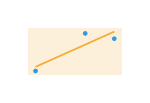
\begin{tikzpicture}[x=1cm,y=1cm]
  \fill[malgray!15] (0,0) rectangle (1.2,0.6);
  \draw[malgray,line width=0.6pt,opacity=0.8] (0.1000,0.1025) -- (1.1000,0.5500);
  \fill[malblue] (0.1000,0.0500) circle[radius=0.03cm];
  \fill[malblue] (0.7309,0.5271) circle[radius=0.03cm];
  \fill[malblue] (1.1000,0.4602) circle[radius=0.03cm];
\end{tikzpicture}} & \textcolor{malgray}{-0.07} & \raisebox{-0.25\height}{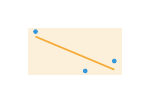
\begin{tikzpicture}[x=1cm,y=1cm]
  \fill[malgray!15] (0,0) rectangle (1.2,0.6);
  \draw[malgray,line width=0.6pt,opacity=0.8] (0.1000,0.4865) -- (1.1000,0.0673);
  \fill[malblue] (0.1000,0.5500) circle[radius=0.03cm];
  \fill[malblue] (0.7309,0.0500) circle[radius=0.03cm];
  \fill[malblue] (1.1000,0.1758) circle[radius=0.03cm];
\end{tikzpicture}} & \textcolor{malgray}{+0.07} & --- & --- \\
  Afrikaans & IE & OV & \raisebox{-0.25\height}{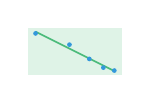
\begin{tikzpicture}[x=1cm,y=1cm]
  \fill[malgreen!15] (0,0) rectangle (1.2,0.6);
  \draw[malgreen,line width=0.6pt,opacity=0.8] (0.1000,0.5500) -- (1.1000,0.0500);
  \fill[malblue] (0.1000,0.5271) circle[radius=0.03cm];
  \fill[malblue] (0.5307,0.3845) circle[radius=0.03cm];
  \fill[malblue] (0.7826,0.2032) circle[radius=0.03cm];
  \fill[malblue] (0.9614,0.0924) circle[radius=0.03cm];
  \fill[malblue] (1.1000,0.0555) circle[radius=0.03cm];
\end{tikzpicture}} & \textcolor{malgreen}{+0.18} & \raisebox{-0.25\height}{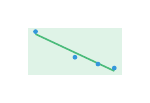
\begin{tikzpicture}[x=1cm,y=1cm]
  \fill[malgreen!15] (0,0) rectangle (1.2,0.6);
  \draw[malgreen,line width=0.6pt,opacity=0.8] (0.1000,0.5181) -- (1.1000,0.0500);
  \fill[malblue] (0.1000,0.5500) circle[radius=0.03cm];
  \fill[malblue] (0.6000,0.2242) circle[radius=0.03cm];
  \fill[malblue] (0.8925,0.1378) circle[radius=0.03cm];
  \fill[malblue] (1.1000,0.0874) circle[radius=0.03cm];
\end{tikzpicture}} & \textcolor{malgreen}{+0.19} & \raisebox{-0.25\height}{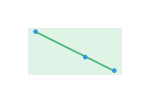
\begin{tikzpicture}[x=1cm,y=1cm]
  \fill[malgreen!15] (0,0) rectangle (1.2,0.6);
  \draw[malgreen,line width=0.6pt,opacity=0.8] (0.1000,0.5471) -- (1.1000,0.0500);
  \fill[malblue] (0.1000,0.5500) circle[radius=0.03cm];
  \fill[malblue] (0.7309,0.2256) circle[radius=0.03cm];
  \fill[malblue] (1.1000,0.0550) circle[radius=0.03cm];
\end{tikzpicture}} & \textcolor{malgreen}{+0.55} \\
  Akkadian & Afroasia & OV & \raisebox{-0.25\height}{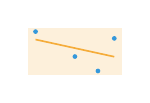
\begin{tikzpicture}[x=1cm,y=1cm]
  \fill[malgray!15] (0,0) rectangle (1.2,0.6);
  \draw[malgray,line width=0.6pt,opacity=0.8] (0.1000,0.4496) -- (1.1000,0.2310);
  \fill[malblue] (0.1000,0.5500) circle[radius=0.03cm];
  \fill[malblue] (0.6000,0.2334) circle[radius=0.03cm];
  \fill[malblue] (0.8925,0.0500) circle[radius=0.03cm];
  \fill[malblue] (1.1000,0.4639) circle[radius=0.03cm];
\end{tikzpicture}} & \textcolor{malgray}{+0.05} & \raisebox{-0.25\height}{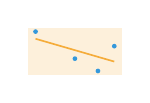
\begin{tikzpicture}[x=1cm,y=1cm]
  \fill[malgray!15] (0,0) rectangle (1.2,0.6);
  \draw[malgray,line width=0.6pt,opacity=0.8] (0.1000,0.4590) -- (1.1000,0.1694);
  \fill[malblue] (0.1000,0.5500) circle[radius=0.03cm];
  \fill[malblue] (0.6000,0.2066) circle[radius=0.03cm];
  \fill[malblue] (0.8925,0.0500) circle[radius=0.03cm];
  \fill[malblue] (1.1000,0.3654) circle[radius=0.03cm];
\end{tikzpicture}} & \textcolor{malgray}{+0.09} & --- & --- \\
  Albanian & IE & VO & \raisebox{-0.25\height}{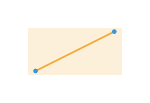
\begin{tikzpicture}[x=1cm,y=1cm]
  \fill[malgray!15] (0,0) rectangle (1.2,0.6);
  \draw[malgray,line width=0.6pt,opacity=0.8] (0.1000,0.0500) -- (1.1000,0.5500);
  \fill[malblue] (0.1000,0.0500) circle[radius=0.03cm];
  \fill[malblue] (1.1000,0.5500) circle[radius=0.03cm];
\end{tikzpicture}} & \textcolor{malgray}{-0.05} & \raisebox{-0.25\height}{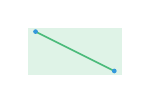
\begin{tikzpicture}[x=1cm,y=1cm]
  \fill[malgreen!15] (0,0) rectangle (1.2,0.6);
  \draw[malgreen,line width=0.6pt,opacity=0.8] (0.1000,0.5500) -- (1.1000,0.0500);
  \fill[malblue] (0.1000,0.5500) circle[radius=0.03cm];
  \fill[malblue] (1.1000,0.0500) circle[radius=0.03cm];
\end{tikzpicture}} & \textcolor{malgreen}{+0.12} & \raisebox{-0.25\height}{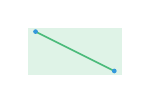
\begin{tikzpicture}[x=1cm,y=1cm]
  \fill[malgreen!15] (0,0) rectangle (1.2,0.6);
  \draw[malgreen,line width=0.6pt,opacity=0.8] (0.1000,0.5500) -- (1.1000,0.0500);
  \fill[malblue] (0.1000,0.5500) circle[radius=0.03cm];
  \fill[malblue] (1.1000,0.0500) circle[radius=0.03cm];
\end{tikzpicture}} & \textcolor{malgreen}{+0.47} \\
  Amharic & Afroasia & OV & \raisebox{-0.25\height}{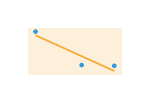
\begin{tikzpicture}[x=1cm,y=1cm]
  \fill[malgray!15] (0,0) rectangle (1.2,0.6);
  \draw[malgray,line width=0.6pt,opacity=0.8] (0.1000,0.5031) -- (1.1000,0.0500);
  \fill[malblue] (0.1000,0.5500) circle[radius=0.03cm];
  \fill[malblue] (0.6850,0.1252) circle[radius=0.03cm];
  \fill[malblue] (1.1000,0.1160) circle[radius=0.03cm];
\end{tikzpicture}} & \textcolor{malgray}{+0.07} & \raisebox{-0.25\height}{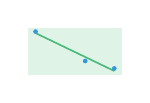
\begin{tikzpicture}[x=1cm,y=1cm]
  \fill[malgreen!15] (0,0) rectangle (1.2,0.6);
  \draw[malgreen,line width=0.6pt,opacity=0.8] (0.1000,0.5312) -- (1.1000,0.0500);
  \fill[malblue] (0.1000,0.5500) circle[radius=0.03cm];
  \fill[malblue] (0.7309,0.1767) circle[radius=0.03cm];
  \fill[malblue] (1.1000,0.0821) circle[radius=0.03cm];
\end{tikzpicture}} & \textcolor{malgreen}{+0.30} & \raisebox{-0.25\height}{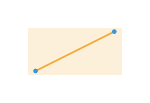
\begin{tikzpicture}[x=1cm,y=1cm]
  \fill[malgray!15] (0,0) rectangle (1.2,0.6);
  \draw[malgray,line width=0.6pt,opacity=0.8] (0.1000,0.0500) -- (1.1000,0.5500);
  \fill[malblue] (0.1000,0.0500) circle[radius=0.03cm];
  \fill[malblue] (1.1000,0.5500) circle[radius=0.03cm];
\end{tikzpicture}} & \textcolor{malgray}{-0.00} \\
  AncientGreek & IE & mix & \raisebox{-0.25\height}{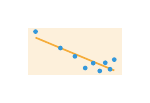
\begin{tikzpicture}[x=1cm,y=1cm]
  \fill[malgray!15] (0,0) rectangle (1.2,0.6);
  \draw[malgray,line width=0.6pt,opacity=0.8] (0.1000,0.4739) -- (1.1000,0.0567);
  \fill[malblue] (0.1000,0.5500) circle[radius=0.03cm];
  \fill[malblue] (0.4155,0.3413) circle[radius=0.03cm];
  \fill[malblue] (0.6000,0.2356) circle[radius=0.03cm];
  \fill[malblue] (0.7309,0.0877) circle[radius=0.03cm];
  \fill[malblue] (0.8325,0.1494) circle[radius=0.03cm];
  \fill[malblue] (0.9155,0.0500) circle[radius=0.03cm];
  \fill[malblue] (0.9856,0.1543) circle[radius=0.03cm];
  \fill[malblue] (1.0464,0.0720) circle[radius=0.03cm];
  \fill[malblue] (1.1000,0.1942) circle[radius=0.03cm];
\end{tikzpicture}} & \textcolor{malgray}{+0.05} & \raisebox{-0.25\height}{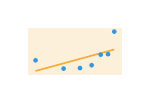
\begin{tikzpicture}[x=1cm,y=1cm]
  \fill[malgray!15] (0,0) rectangle (1.2,0.6);
  \draw[malgray,line width=0.6pt,opacity=0.8] (0.1000,0.0500) -- (1.1000,0.3229);
  \fill[malblue] (0.1000,0.1851) circle[radius=0.03cm];
  \fill[malblue] (0.4562,0.0805) circle[radius=0.03cm];
  \fill[malblue] (0.6646,0.0872) circle[radius=0.03cm];
  \fill[malblue] (0.8124,0.1227) circle[radius=0.03cm];
  \fill[malblue] (0.9271,0.2573) circle[radius=0.03cm];
  \fill[malblue] (1.0208,0.2631) circle[radius=0.03cm];
  \fill[malblue] (1.1000,0.5500) circle[radius=0.03cm];
\end{tikzpicture}} & \textcolor{malgray}{-0.06} & \raisebox{-0.25\height}{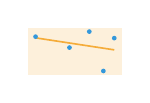
\begin{tikzpicture}[x=1cm,y=1cm]
  \fill[malgray!15] (0,0) rectangle (1.2,0.6);
  \draw[malgray,line width=0.6pt,opacity=0.8] (0.1000,0.4708) -- (1.1000,0.3182);
  \fill[malblue] (0.1000,0.4858) circle[radius=0.03cm];
  \fill[malblue] (0.5307,0.3471) circle[radius=0.03cm];
  \fill[malblue] (0.7826,0.5500) circle[radius=0.03cm];
  \fill[malblue] (0.9614,0.0500) circle[radius=0.03cm];
  \fill[malblue] (1.1000,0.4672) circle[radius=0.03cm];
\end{tikzpicture}} & \textcolor{malgray}{+0.01} \\
  AncientHebrew & Afroasia & VO & \raisebox{-0.25\height}{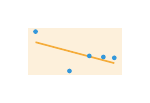
\begin{tikzpicture}[x=1cm,y=1cm]
  \fill[malgray!15] (0,0) rectangle (1.2,0.6);
  \draw[malgray,line width=0.6pt,opacity=0.8] (0.1000,0.4153) -- (1.1000,0.1497);
  \fill[malblue] (0.1000,0.5500) circle[radius=0.03cm];
  \fill[malblue] (0.5307,0.0500) circle[radius=0.03cm];
  \fill[malblue] (0.7826,0.2415) circle[radius=0.03cm];
  \fill[malblue] (0.9614,0.2279) circle[radius=0.03cm];
  \fill[malblue] (1.1000,0.2170) circle[radius=0.03cm];
\end{tikzpicture}} & \textcolor{malgray}{+0.03} & \raisebox{-0.25\height}{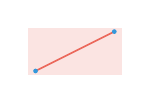
\begin{tikzpicture}[x=1cm,y=1cm]
  \fill[malred!15] (0,0) rectangle (1.2,0.6);
  \draw[malred,line width=0.6pt,opacity=0.8] (0.1000,0.0500) -- (1.1000,0.5500);
  \fill[malblue] (0.1000,0.0500) circle[radius=0.03cm];
  \fill[malblue] (1.1000,0.5500) circle[radius=0.03cm];
\end{tikzpicture}} & \textcolor{malred}{-0.13} & \raisebox{-0.25\height}{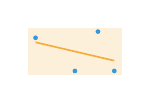
\begin{tikzpicture}[x=1cm,y=1cm]
  \fill[malgray!15] (0,0) rectangle (1.2,0.6);
  \draw[malgray,line width=0.6pt,opacity=0.8] (0.1000,0.4142) -- (1.1000,0.1810);
  \fill[malblue] (0.1000,0.4715) circle[radius=0.03cm];
  \fill[malblue] (0.6000,0.0500) circle[radius=0.03cm];
  \fill[malblue] (0.8925,0.5500) circle[radius=0.03cm];
  \fill[malblue] (1.1000,0.0507) circle[radius=0.03cm];
\end{tikzpicture}} & \textcolor{malgray}{+0.03} \\
  Arabic & Afroasia & VO & \raisebox{-0.25\height}{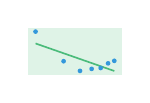
\begin{tikzpicture}[x=1cm,y=1cm]
  \fill[malgreen!15] (0,0) rectangle (1.2,0.6);
  \draw[malgreen,line width=0.6pt,opacity=0.8] (0.1000,0.3995) -- (1.1000,0.0500);
  \fill[malblue] (0.1000,0.5500) circle[radius=0.03cm];
  \fill[malblue] (0.4562,0.1740) circle[radius=0.03cm];
  \fill[malblue] (0.6646,0.0510) circle[radius=0.03cm];
  \fill[malblue] (0.8124,0.0767) circle[radius=0.03cm];
  \fill[malblue] (0.9271,0.0880) circle[radius=0.03cm];
  \fill[malblue] (1.0208,0.1468) circle[radius=0.03cm];
  \fill[malblue] (1.1000,0.1789) circle[radius=0.03cm];
\end{tikzpicture}} & \textcolor{malgreen}{+0.16} & \raisebox{-0.25\height}{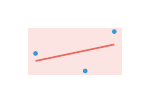
\begin{tikzpicture}[x=1cm,y=1cm]
  \fill[malred!15] (0,0) rectangle (1.2,0.6);
  \draw[malred,line width=0.6pt,opacity=0.8] (0.1000,0.1771) -- (1.1000,0.3865);
  \fill[malblue] (0.1000,0.2727) circle[radius=0.03cm];
  \fill[malblue] (0.7309,0.0500) circle[radius=0.03cm];
  \fill[malblue] (1.1000,0.5500) circle[radius=0.03cm];
\end{tikzpicture}} & \textcolor{malred}{-0.12} & \raisebox{-0.25\height}{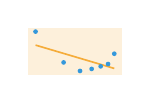
\begin{tikzpicture}[x=1cm,y=1cm]
  \fill[malgray!15] (0,0) rectangle (1.2,0.6);
  \draw[malgray,line width=0.6pt,opacity=0.8] (0.1000,0.3785) -- (1.1000,0.0821);
  \fill[malblue] (0.1000,0.5500) circle[radius=0.03cm];
  \fill[malblue] (0.4562,0.1588) circle[radius=0.03cm];
  \fill[malblue] (0.6646,0.0500) circle[radius=0.03cm];
  \fill[malblue] (0.8124,0.0761) circle[radius=0.03cm];
  \fill[malblue] (0.9271,0.1088) circle[radius=0.03cm];
  \fill[malblue] (1.0208,0.1382) circle[radius=0.03cm];
  \fill[malblue] (1.1000,0.2690) circle[radius=0.03cm];
\end{tikzpicture}} & \textcolor{malgray}{+0.10} \\
  Arhuaco & South-Am & OV & \raisebox{-0.25\height}{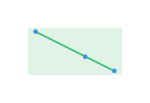
\begin{tikzpicture}[x=1cm,y=1cm]
  \fill[malgreen!15] (0,0) rectangle (1.2,0.6);
  \draw[malgreen,line width=0.6pt,opacity=0.8] (0.1000,0.5489) -- (1.1000,0.0500);
  \fill[malblue] (0.1000,0.5500) circle[radius=0.03cm];
  \fill[malblue] (0.7309,0.2311) circle[radius=0.03cm];
  \fill[malblue] (1.1000,0.0519) circle[radius=0.03cm];
\end{tikzpicture}} & \textcolor{malgreen}{+0.13} & \raisebox{-0.25\height}{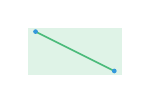
\begin{tikzpicture}[x=1cm,y=1cm]
  \fill[malgreen!15] (0,0) rectangle (1.2,0.6);
  \draw[malgreen,line width=0.6pt,opacity=0.8] (0.1000,0.5500) -- (1.1000,0.0500);
  \fill[malblue] (0.1000,0.5500) circle[radius=0.03cm];
  \fill[malblue] (1.1000,0.0500) circle[radius=0.03cm];
\end{tikzpicture}} & \textcolor{malgreen}{+0.25} & --- & --- \\
  Armenian & IE & mix & \raisebox{-0.25\height}{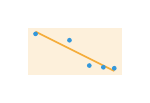
\begin{tikzpicture}[x=1cm,y=1cm]
  \fill[malgray!15] (0,0) rectangle (1.2,0.6);
  \draw[malgray,line width=0.6pt,opacity=0.8] (0.1000,0.5500) -- (1.1000,0.0500);
  \fill[malblue] (0.1000,0.5213) circle[radius=0.03cm];
  \fill[malblue] (0.5307,0.4405) circle[radius=0.03cm];
  \fill[malblue] (0.7826,0.1191) circle[radius=0.03cm];
  \fill[malblue] (0.9614,0.0972) circle[radius=0.03cm];
  \fill[malblue] (1.1000,0.0846) circle[radius=0.03cm];
\end{tikzpicture}} & \textcolor{malgray}{+0.06} & \raisebox{-0.25\height}{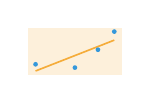
\begin{tikzpicture}[x=1cm,y=1cm]
  \fill[malgray!15] (0,0) rectangle (1.2,0.6);
  \draw[malgray,line width=0.6pt,opacity=0.8] (0.1000,0.0500) -- (1.1000,0.4416);
  \fill[malblue] (0.1000,0.1348) circle[radius=0.03cm];
  \fill[malblue] (0.6000,0.0929) circle[radius=0.03cm];
  \fill[malblue] (0.8925,0.3200) circle[radius=0.03cm];
  \fill[malblue] (1.1000,0.5500) circle[radius=0.03cm];
\end{tikzpicture}} & \textcolor{malgray}{-0.05} & \raisebox{-0.25\height}{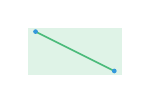
\begin{tikzpicture}[x=1cm,y=1cm]
  \fill[malgreen!15] (0,0) rectangle (1.2,0.6);
  \draw[malgreen,line width=0.6pt,opacity=0.8] (0.1000,0.5500) -- (1.1000,0.0500);
  \fill[malblue] (0.1000,0.5500) circle[radius=0.03cm];
  \fill[malblue] (1.1000,0.0500) circle[radius=0.03cm];
\end{tikzpicture}} & \textcolor{malgreen}{+0.15} \\
  Bambara & Nig-Co. & OV & \raisebox{-0.25\height}{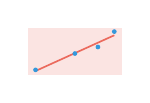
\begin{tikzpicture}[x=1cm,y=1cm]
  \fill[malred!15] (0,0) rectangle (1.2,0.6);
  \draw[malred,line width=0.6pt,opacity=0.8] (0.1000,0.0500) -- (1.1000,0.5036);
  \fill[malblue] (0.1000,0.0641) circle[radius=0.03cm];
  \fill[malblue] (0.6000,0.2715) circle[radius=0.03cm];
  \fill[malblue] (0.8925,0.3544) circle[radius=0.03cm];
  \fill[malblue] (1.1000,0.5500) circle[radius=0.03cm];
\end{tikzpicture}} & \textcolor{malred}{-0.29} & \raisebox{-0.25\height}{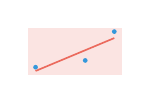
\begin{tikzpicture}[x=1cm,y=1cm]
  \fill[malred!15] (0,0) rectangle (1.2,0.6);
  \draw[malred,line width=0.6pt,opacity=0.8] (0.1000,0.0500) -- (1.1000,0.4680);
  \fill[malblue] (0.1000,0.0980) circle[radius=0.03cm];
  \fill[malblue] (0.7309,0.1837) circle[radius=0.03cm];
  \fill[malblue] (1.1000,0.5500) circle[radius=0.03cm];
\end{tikzpicture}} & \textcolor{malred}{-0.51} & \raisebox{-0.25\height}{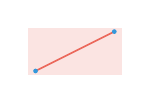
\begin{tikzpicture}[x=1cm,y=1cm]
  \fill[malred!15] (0,0) rectangle (1.2,0.6);
  \draw[malred,line width=0.6pt,opacity=0.8] (0.1000,0.0500) -- (1.1000,0.5500);
  \fill[malblue] (0.1000,0.0500) circle[radius=0.03cm];
  \fill[malblue] (1.1000,0.5500) circle[radius=0.03cm];
\end{tikzpicture}} & \textcolor{malred}{-0.20} \\
  Basque & Other & OV & \raisebox{-0.25\height}{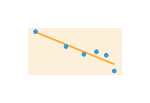
\begin{tikzpicture}[x=1cm,y=1cm]
  \fill[malgray!15] (0,0) rectangle (1.2,0.6);
  \draw[malgray,line width=0.6pt,opacity=0.8] (0.1000,0.5438) -- (1.1000,0.1361);
  \fill[malblue] (0.1000,0.5500) circle[radius=0.03cm];
  \fill[malblue] (0.4869,0.3603) circle[radius=0.03cm];
  \fill[malblue] (0.7131,0.2608) circle[radius=0.03cm];
  \fill[malblue] (0.8737,0.2948) circle[radius=0.03cm];
  \fill[malblue] (0.9982,0.2497) circle[radius=0.03cm];
  \fill[malblue] (1.1000,0.0500) circle[radius=0.03cm];
\end{tikzpicture}} & \textcolor{malgray}{+0.06} & \raisebox{-0.25\height}{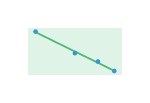
\begin{tikzpicture}[x=1cm,y=1cm]
  \fill[malgreen!15] (0,0) rectangle (1.2,0.6);
  \draw[malgreen,line width=0.6pt,opacity=0.8] (0.1000,0.5426) -- (1.1000,0.0520);
  \fill[malblue] (0.1000,0.5500) circle[radius=0.03cm];
  \fill[malblue] (0.6000,0.2759) circle[radius=0.03cm];
  \fill[malblue] (0.8925,0.1698) circle[radius=0.03cm];
  \fill[malblue] (1.1000,0.0500) circle[radius=0.03cm];
\end{tikzpicture}} & \textcolor{malgreen}{+0.18} & \raisebox{-0.25\height}{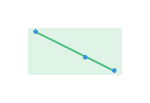
\begin{tikzpicture}[x=1cm,y=1cm]
  \fill[malgreen!15] (0,0) rectangle (1.2,0.6);
  \draw[malgreen,line width=0.6pt,opacity=0.8] (0.1000,0.5466) -- (1.1000,0.0500);
  \fill[malblue] (0.1000,0.5500) circle[radius=0.03cm];
  \fill[malblue] (0.7309,0.2240) circle[radius=0.03cm];
  \fill[malblue] (1.1000,0.0559) circle[radius=0.03cm];
\end{tikzpicture}} & \textcolor{malgreen}{+0.11} \\
  Bavarian & IE & mix & \raisebox{-0.25\height}{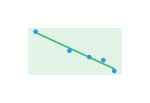
\begin{tikzpicture}[x=1cm,y=1cm]
  \fill[malgreen!15] (0,0) rectangle (1.2,0.6);
  \draw[malgreen,line width=0.6pt,opacity=0.8] (0.1000,0.5387) -- (1.1000,0.0774);
  \fill[malblue] (0.1000,0.5500) circle[radius=0.03cm];
  \fill[malblue] (0.5307,0.3074) circle[radius=0.03cm];
  \fill[malblue] (0.7826,0.2266) circle[radius=0.03cm];
  \fill[malblue] (0.9614,0.1874) circle[radius=0.03cm];
  \fill[malblue] (1.1000,0.0500) circle[radius=0.03cm];
\end{tikzpicture}} & \textcolor{malgreen}{+0.13} & \raisebox{-0.25\height}{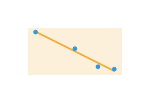
\begin{tikzpicture}[x=1cm,y=1cm]
  \fill[malgray!15] (0,0) rectangle (1.2,0.6);
  \draw[malgray,line width=0.6pt,opacity=0.8] (0.1000,0.5500) -- (1.1000,0.0500);
  \fill[malblue] (0.1000,0.5438) circle[radius=0.03cm];
  \fill[malblue] (0.6000,0.3331) circle[radius=0.03cm];
  \fill[malblue] (0.8925,0.1040) circle[radius=0.03cm];
  \fill[malblue] (1.1000,0.0729) circle[radius=0.03cm];
\end{tikzpicture}} & \textcolor{malgray}{+0.09} & \raisebox{-0.25\height}{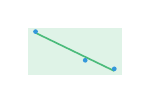
\begin{tikzpicture}[x=1cm,y=1cm]
  \fill[malgreen!15] (0,0) rectangle (1.2,0.6);
  \draw[malgreen,line width=0.6pt,opacity=0.8] (0.1000,0.5342) -- (1.1000,0.0500);
  \fill[malblue] (0.1000,0.5500) circle[radius=0.03cm];
  \fill[malblue] (0.7309,0.1860) circle[radius=0.03cm];
  \fill[malblue] (1.1000,0.0769) circle[radius=0.03cm];
\end{tikzpicture}} & \textcolor{malgreen}{+0.75} \\
  Beja & Afroasia & OV & \raisebox{-0.25\height}{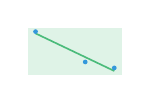
\begin{tikzpicture}[x=1cm,y=1cm]
  \fill[malgreen!15] (0,0) rectangle (1.2,0.6);
  \draw[malgreen,line width=0.6pt,opacity=0.8] (0.1000,0.5272) -- (1.1000,0.0500);
  \fill[malblue] (0.1000,0.5500) circle[radius=0.03cm];
  \fill[malblue] (0.7309,0.1643) circle[radius=0.03cm];
  \fill[malblue] (1.1000,0.0890) circle[radius=0.03cm];
\end{tikzpicture}} & \textcolor{malgreen}{+0.38} & \raisebox{-0.25\height}{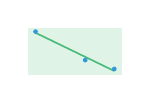
\begin{tikzpicture}[x=1cm,y=1cm]
  \fill[malgreen!15] (0,0) rectangle (1.2,0.6);
  \draw[malgreen,line width=0.6pt,opacity=0.8] (0.1000,0.5349) -- (1.1000,0.0500);
  \fill[malblue] (0.1000,0.5500) circle[radius=0.03cm];
  \fill[malblue] (0.7309,0.1882) circle[radius=0.03cm];
  \fill[malblue] (1.1000,0.0757) circle[radius=0.03cm];
\end{tikzpicture}} & \textcolor{malgreen}{+0.40} & --- & --- \\
  Belarusian & IE & VO & \raisebox{-0.25\height}{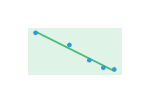
\begin{tikzpicture}[x=1cm,y=1cm]
  \fill[malgreen!15] (0,0) rectangle (1.2,0.6);
  \draw[malgreen,line width=0.6pt,opacity=0.8] (0.1000,0.5500) -- (1.1000,0.0500);
  \fill[malblue] (0.1000,0.5347) circle[radius=0.03cm];
  \fill[malblue] (0.5307,0.3806) circle[radius=0.03cm];
  \fill[malblue] (0.7826,0.1869) circle[radius=0.03cm];
  \fill[malblue] (0.9614,0.0911) circle[radius=0.03cm];
  \fill[malblue] (1.1000,0.0695) circle[radius=0.03cm];
\end{tikzpicture}} & \textcolor{malgreen}{+0.18} & \raisebox{-0.25\height}{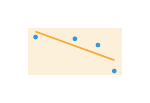
\begin{tikzpicture}[x=1cm,y=1cm]
  \fill[malgray!15] (0,0) rectangle (1.2,0.6);
  \draw[malgray,line width=0.6pt,opacity=0.8] (0.1000,0.5500) -- (1.1000,0.1873);
  \fill[malblue] (0.1000,0.4808) circle[radius=0.03cm];
  \fill[malblue] (0.6000,0.4588) circle[radius=0.03cm];
  \fill[malblue] (0.8925,0.3790) circle[radius=0.03cm];
  \fill[malblue] (1.1000,0.0500) circle[radius=0.03cm];
\end{tikzpicture}} & \textcolor{malgray}{+0.09} & \raisebox{-0.25\height}{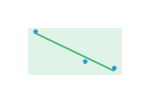
\begin{tikzpicture}[x=1cm,y=1cm]
  \fill[malgreen!15] (0,0) rectangle (1.2,0.6);
  \draw[malgreen,line width=0.6pt,opacity=0.8] (0.1000,0.5290) -- (1.1000,0.0500);
  \fill[malblue] (0.1000,0.5500) circle[radius=0.03cm];
  \fill[malblue] (0.7309,0.1698) circle[radius=0.03cm];
  \fill[malblue] (1.1000,0.0859) circle[radius=0.03cm];
\end{tikzpicture}} & \textcolor{malgreen}{+0.34} \\
  Bhojpuri & IE & OV & \raisebox{-0.25\height}{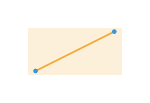
\begin{tikzpicture}[x=1cm,y=1cm]
  \fill[malgray!15] (0,0) rectangle (1.2,0.6);
  \draw[malgray,line width=0.6pt,opacity=0.8] (0.1000,0.0500) -- (1.1000,0.5500);
  \fill[malblue] (0.1000,0.0500) circle[radius=0.03cm];
  \fill[malblue] (1.1000,0.5500) circle[radius=0.03cm];
\end{tikzpicture}} & \textcolor{malgray}{-0.04} & \raisebox{-0.25\height}{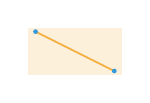
\begin{tikzpicture}[x=1cm,y=1cm]
  \fill[malgray!15] (0,0) rectangle (1.2,0.6);
  \draw[malgray,line width=0.6pt,opacity=0.8] (0.1000,0.5500) -- (1.1000,0.0500);
  \fill[malblue] (0.1000,0.5500) circle[radius=0.03cm];
  \fill[malblue] (1.1000,0.0500) circle[radius=0.03cm];
\end{tikzpicture}} & \textcolor{malgray}{+0.09} & --- & --- \\
  Borôro & South-Am & OV & \raisebox{-0.25\height}{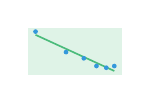
\begin{tikzpicture}[x=1cm,y=1cm]
  \fill[malgreen!15] (0,0) rectangle (1.2,0.6);
  \draw[malgreen,line width=0.6pt,opacity=0.8] (0.1000,0.5086) -- (1.1000,0.0500);
  \fill[malblue] (0.1000,0.5500) circle[radius=0.03cm];
  \fill[malblue] (0.4869,0.2898) circle[radius=0.03cm];
  \fill[malblue] (0.7131,0.2111) circle[radius=0.03cm];
  \fill[malblue] (0.8737,0.1131) circle[radius=0.03cm];
  \fill[malblue] (0.9982,0.0911) circle[radius=0.03cm];
  \fill[malblue] (1.1000,0.1125) circle[radius=0.03cm];
\end{tikzpicture}} & \textcolor{malgreen}{+0.13} & \raisebox{-0.25\height}{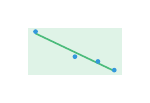
\begin{tikzpicture}[x=1cm,y=1cm]
  \fill[malgreen!15] (0,0) rectangle (1.2,0.6);
  \draw[malgreen,line width=0.6pt,opacity=0.8] (0.1000,0.5263) -- (1.1000,0.0500);
  \fill[malblue] (0.1000,0.5500) circle[radius=0.03cm];
  \fill[malblue] (0.6000,0.2316) circle[radius=0.03cm];
  \fill[malblue] (0.8925,0.1708) circle[radius=0.03cm];
  \fill[malblue] (1.1000,0.0608) circle[radius=0.03cm];
\end{tikzpicture}} & \textcolor{malgreen}{+0.23} & \raisebox{-0.25\height}{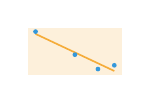
\begin{tikzpicture}[x=1cm,y=1cm]
  \fill[malgray!15] (0,0) rectangle (1.2,0.6);
  \draw[malgray,line width=0.6pt,opacity=0.8] (0.1000,0.5206) -- (1.1000,0.0500);
  \fill[malblue] (0.1000,0.5500) circle[radius=0.03cm];
  \fill[malblue] (0.6000,0.2568) circle[radius=0.03cm];
  \fill[malblue] (0.8925,0.0745) circle[radius=0.03cm];
  \fill[malblue] (1.1000,0.1222) circle[radius=0.03cm];
\end{tikzpicture}} & \textcolor{malgray}{+0.10} \\
  Breton & IE & VO & \raisebox{-0.25\height}{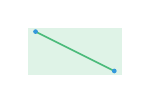
\begin{tikzpicture}[x=1cm,y=1cm]
  \fill[malgreen!15] (0,0) rectangle (1.2,0.6);
  \draw[malgreen,line width=0.6pt,opacity=0.8] (0.1000,0.5500) -- (1.1000,0.0500);
  \fill[malblue] (0.1000,0.5500) circle[radius=0.03cm];
  \fill[malblue] (1.1000,0.0500) circle[radius=0.03cm];
\end{tikzpicture}} & \textcolor{malgreen}{+0.12} & --- & --- & \raisebox{-0.25\height}{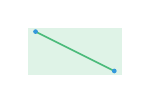
\begin{tikzpicture}[x=1cm,y=1cm]
  \fill[malgreen!15] (0,0) rectangle (1.2,0.6);
  \draw[malgreen,line width=0.6pt,opacity=0.8] (0.1000,0.5500) -- (1.1000,0.0500);
  \fill[malblue] (0.1000,0.5500) circle[radius=0.03cm];
  \fill[malblue] (1.1000,0.0500) circle[radius=0.03cm];
\end{tikzpicture}} & \textcolor{malgreen}{+0.20} \\
  Buglere & South-Am & OV & \raisebox{-0.25\height}{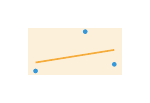
\begin{tikzpicture}[x=1cm,y=1cm]
  \fill[malgray!15] (0,0) rectangle (1.2,0.6);
  \draw[malgray,line width=0.6pt,opacity=0.8] (0.1000,0.1575) -- (1.1000,0.3179);
  \fill[malblue] (0.1000,0.0500) circle[radius=0.03cm];
  \fill[malblue] (0.7309,0.5500) circle[radius=0.03cm];
  \fill[malblue] (1.1000,0.1342) circle[radius=0.03cm];
\end{tikzpicture}} & \textcolor{malgray}{-0.01} & \raisebox{-0.25\height}{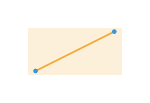
\begin{tikzpicture}[x=1cm,y=1cm]
  \fill[malgray!15] (0,0) rectangle (1.2,0.6);
  \draw[malgray,line width=0.6pt,opacity=0.8] (0.1000,0.0500) -- (1.1000,0.5500);
  \fill[malblue] (0.1000,0.0500) circle[radius=0.03cm];
  \fill[malblue] (1.1000,0.5500) circle[radius=0.03cm];
\end{tikzpicture}} & \textcolor{malgray}{-0.05} & --- & --- \\
  Bulgarian & IE & VO & \raisebox{-0.25\height}{\begin{tikzpicture}[x=1cm,y=1cm]
  \fill[malgreen!15] (0,0) rectangle (1.2,0.6);
  \draw[malgreen,line width=0.6pt,opacity=0.8] (0.1000,0.5500) -- (1.1000,0.0796);
  \fill[malblue] (0.1000,0.4973) circle[radius=0.03cm];
  \fill[malblue] (0.5307,0.4360) circle[radius=0.03cm];
  \fill[malblue] (0.7826,0.2463) circle[radius=0.03cm];
  \fill[malblue] (0.9614,0.1210) circle[radius=0.03cm];
  \fill[malblue] (1.1000,0.0500) circle[radius=0.03cm];
\end{tikzpicture}} & \textcolor{malgreen}{+0.17} & \raisebox{-0.25\height}{\begin{tikzpicture}[x=1cm,y=1cm]
  \fill[malgreen!15] (0,0) rectangle (1.2,0.6);
  \draw[malgreen,line width=0.6pt,opacity=0.8] (0.1000,0.5035) -- (1.1000,0.0500);
  \fill[malblue] (0.1000,0.5500) circle[radius=0.03cm];
  \fill[malblue] (0.6000,0.2034) circle[radius=0.03cm];
  \fill[malblue] (0.8925,0.0967) circle[radius=0.03cm];
  \fill[malblue] (1.1000,0.1243) circle[radius=0.03cm];
\end{tikzpicture}} & \textcolor{malgreen}{+0.17} & \raisebox{-0.25\height}{\begin{tikzpicture}[x=1cm,y=1cm]
  \fill[malgreen!15] (0,0) rectangle (1.2,0.6);
  \draw[malgreen,line width=0.6pt,opacity=0.8] (0.1000,0.5277) -- (1.1000,0.0500);
  \fill[malblue] (0.1000,0.5500) circle[radius=0.03cm];
  \fill[malblue] (0.7309,0.1660) circle[radius=0.03cm];
  \fill[malblue] (1.1000,0.0880) circle[radius=0.03cm];
\end{tikzpicture}} & \textcolor{malgreen}{+0.33} \\
  Buryat & Other & OV & \raisebox{-0.25\height}{\begin{tikzpicture}[x=1cm,y=1cm]
  \fill[malgreen!15] (0,0) rectangle (1.2,0.6);
  \draw[malgreen,line width=0.6pt,opacity=0.8] (0.1000,0.5076) -- (1.1000,0.0500);
  \fill[malblue] (0.1000,0.5500) circle[radius=0.03cm];
  \fill[malblue] (0.7309,0.1042) circle[radius=0.03cm];
  \fill[malblue] (1.1000,0.1224) circle[radius=0.03cm];
\end{tikzpicture}} & \textcolor{malgreen}{+0.16} & \raisebox{-0.25\height}{\begin{tikzpicture}[x=1cm,y=1cm]
  \fill[malgreen!15] (0,0) rectangle (1.2,0.6);
  \draw[malgreen,line width=0.6pt,opacity=0.8] (0.1000,0.5222) -- (1.1000,0.0500);
  \fill[malblue] (0.1000,0.5500) circle[radius=0.03cm];
  \fill[malblue] (0.7309,0.1491) circle[radius=0.03cm];
  \fill[malblue] (1.1000,0.0974) circle[radius=0.03cm];
\end{tikzpicture}} & \textcolor{malgreen}{+0.19} & --- & --- \\
  Cantonese & Sino-Aus & VO & \raisebox{-0.25\height}{\begin{tikzpicture}[x=1cm,y=1cm]
  \fill[malgray!15] (0,0) rectangle (1.2,0.6);
  \draw[malgray,line width=0.6pt,opacity=0.8] (0.1000,0.1314) -- (1.1000,0.5425);
  \fill[malblue] (0.1000,0.0500) circle[radius=0.03cm];
  \fill[malblue] (0.6000,0.5500) circle[radius=0.03cm];
  \fill[malblue] (0.8925,0.3360) circle[radius=0.03cm];
  \fill[malblue] (1.1000,0.5320) circle[radius=0.03cm];
\end{tikzpicture}} & \textcolor{malgray}{-0.05} & \raisebox{-0.25\height}{\begin{tikzpicture}[x=1cm,y=1cm]
  \fill[malred!15] (0,0) rectangle (1.2,0.6);
  \draw[malred,line width=0.6pt,opacity=0.8] (0.1000,0.0632) -- (1.1000,0.5500);
  \fill[malblue] (0.1000,0.0500) circle[radius=0.03cm];
  \fill[malblue] (0.7309,0.4061) circle[radius=0.03cm];
  \fill[malblue] (1.1000,0.5275) circle[radius=0.03cm];
\end{tikzpicture}} & \textcolor{malred}{-0.24} & \raisebox{-0.25\height}{\begin{tikzpicture}[x=1cm,y=1cm]
  \fill[malgreen!15] (0,0) rectangle (1.2,0.6);
  \draw[malgreen,line width=0.6pt,opacity=0.8] (0.1000,0.5500) -- (1.1000,0.0500);
  \fill[malblue] (0.1000,0.5500) circle[radius=0.03cm];
  \fill[malblue] (1.1000,0.0500) circle[radius=0.03cm];
\end{tikzpicture}} & \textcolor{malgreen}{+0.39} \\
  CappadocianGreek & IE & VO & --- & --- & --- & --- & \raisebox{-0.25\height}{\begin{tikzpicture}[x=1cm,y=1cm]
  \fill[malgreen!15] (0,0) rectangle (1.2,0.6);
  \draw[malgreen,line width=0.6pt,opacity=0.8] (0.1000,0.5500) -- (1.1000,0.0500);
  \fill[malblue] (0.1000,0.5500) circle[radius=0.03cm];
  \fill[malblue] (1.1000,0.0500) circle[radius=0.03cm];
\end{tikzpicture}} & \textcolor{malgreen}{+0.24} \\
  Catalan & IE & VO & \raisebox{-0.25\height}{\begin{tikzpicture}[x=1cm,y=1cm]
  \fill[malgreen!15] (0,0) rectangle (1.2,0.6);
  \draw[malgreen,line width=0.6pt,opacity=0.8] (0.1000,0.5500) -- (1.1000,0.0500);
  \fill[malblue] (0.1000,0.5382) circle[radius=0.03cm];
  \fill[malblue] (0.4869,0.3938) circle[radius=0.03cm];
  \fill[malblue] (0.7131,0.2282) circle[radius=0.03cm];
  \fill[malblue] (0.8737,0.1421) circle[radius=0.03cm];
  \fill[malblue] (0.9982,0.0969) circle[radius=0.03cm];
  \fill[malblue] (1.1000,0.0648) circle[radius=0.03cm];
\end{tikzpicture}} & \textcolor{malgreen}{+0.26} & \raisebox{-0.25\height}{\begin{tikzpicture}[x=1cm,y=1cm]
  \fill[malgreen!15] (0,0) rectangle (1.2,0.6);
  \draw[malgreen,line width=0.6pt,opacity=0.8] (0.1000,0.4868) -- (1.1000,0.0500);
  \fill[malblue] (0.1000,0.5500) circle[radius=0.03cm];
  \fill[malblue] (0.6000,0.1455) circle[radius=0.03cm];
  \fill[malblue] (0.8925,0.1320) circle[radius=0.03cm];
  \fill[malblue] (1.1000,0.1182) circle[radius=0.03cm];
\end{tikzpicture}} & \textcolor{malgreen}{+0.25} & \raisebox{-0.25\height}{\begin{tikzpicture}[x=1cm,y=1cm]
  \fill[malgreen!15] (0,0) rectangle (1.2,0.6);
  \draw[malgreen,line width=0.6pt,opacity=0.8] (0.1000,0.5178) -- (1.1000,0.0500);
  \fill[malblue] (0.1000,0.5500) circle[radius=0.03cm];
  \fill[malblue] (0.6000,0.2158) circle[radius=0.03cm];
  \fill[malblue] (0.8925,0.1557) circle[radius=0.03cm];
  \fill[malblue] (1.1000,0.0772) circle[radius=0.03cm];
\end{tikzpicture}} & \textcolor{malgreen}{+0.36} \\
  Chhintange & Sino-Aus & OV & \raisebox{-0.25\height}{\begin{tikzpicture}[x=1cm,y=1cm]
  \fill[malgreen!15] (0,0) rectangle (1.2,0.6);
  \draw[malgreen,line width=0.6pt,opacity=0.8] (0.1000,0.5500) -- (1.1000,0.0595);
  \fill[malblue] (0.1000,0.5445) circle[radius=0.03cm];
  \fill[malblue] (0.7309,0.2555) circle[radius=0.03cm];
  \fill[malblue] (1.1000,0.0500) circle[radius=0.03cm];
\end{tikzpicture}} & \textcolor{malgreen}{+0.21} & \raisebox{-0.25\height}{\begin{tikzpicture}[x=1cm,y=1cm]
  \fill[malgreen!15] (0,0) rectangle (1.2,0.6);
  \draw[malgreen,line width=0.6pt,opacity=0.8] (0.1000,0.5500) -- (1.1000,0.0550);
  \fill[malblue] (0.1000,0.5471) circle[radius=0.03cm];
  \fill[malblue] (0.7309,0.2456) circle[radius=0.03cm];
  \fill[malblue] (1.1000,0.0500) circle[radius=0.03cm];
\end{tikzpicture}} & \textcolor{malgreen}{+0.19} & --- & --- \\
  Chinese & Sino-Aus & VO & \raisebox{-0.25\height}{\begin{tikzpicture}[x=1cm,y=1cm]
  \fill[malgray!15] (0,0) rectangle (1.2,0.6);
  \draw[malgray,line width=0.6pt,opacity=0.8] (0.1000,0.1766) -- (1.1000,0.4104);
  \fill[malblue] (0.1000,0.0500) circle[radius=0.03cm];
  \fill[malblue] (0.4869,0.5500) circle[radius=0.03cm];
  \fill[malblue] (0.7131,0.2771) circle[radius=0.03cm];
  \fill[malblue] (0.8737,0.2290) circle[radius=0.03cm];
  \fill[malblue] (0.9982,0.3753) circle[radius=0.03cm];
  \fill[malblue] (1.1000,0.4369) circle[radius=0.03cm];
\end{tikzpicture}} & \textcolor{malgray}{-0.04} & \raisebox{-0.25\height}{\begin{tikzpicture}[x=1cm,y=1cm]
  \fill[malred!15] (0,0) rectangle (1.2,0.6);
  \draw[malred,line width=0.6pt,opacity=0.8] (0.1000,0.0500) -- (1.1000,0.5500);
  \fill[malblue] (0.1000,0.0730) circle[radius=0.03cm];
  \fill[malblue] (0.4869,0.1911) circle[radius=0.03cm];
  \fill[malblue] (0.7131,0.3397) circle[radius=0.03cm];
  \fill[malblue] (0.8737,0.4896) circle[radius=0.03cm];
  \fill[malblue] (0.9982,0.5352) circle[radius=0.03cm];
  \fill[malblue] (1.1000,0.5074) circle[radius=0.03cm];
\end{tikzpicture}} & \textcolor{malred}{-0.15} & \raisebox{-0.25\height}{\begin{tikzpicture}[x=1cm,y=1cm]
  \fill[malgreen!15] (0,0) rectangle (1.2,0.6);
  \draw[malgreen,line width=0.6pt,opacity=0.8] (0.1000,0.5500) -- (1.1000,0.0500);
  \fill[malblue] (0.1000,0.5500) circle[radius=0.03cm];
  \fill[malblue] (1.1000,0.0500) circle[radius=0.03cm];
\end{tikzpicture}} & \textcolor{malgreen}{+0.53} \\
  Chukot & Other & mix & \raisebox{-0.25\height}{\begin{tikzpicture}[x=1cm,y=1cm]
  \fill[malgray!15] (0,0) rectangle (1.2,0.6);
  \draw[malgray,line width=0.6pt,opacity=0.8] (0.1000,0.0662) -- (1.1000,0.5500);
  \fill[malblue] (0.1000,0.0500) circle[radius=0.03cm];
  \fill[malblue] (0.7309,0.4154) circle[radius=0.03cm];
  \fill[malblue] (1.1000,0.5223) circle[radius=0.03cm];
\end{tikzpicture}} & \textcolor{malgray}{-0.05} & \raisebox{-0.25\height}{\begin{tikzpicture}[x=1cm,y=1cm]
  \fill[malgray!15] (0,0) rectangle (1.2,0.6);
  \draw[malgray,line width=0.6pt,opacity=0.8] (0.1000,0.5500) -- (1.1000,0.0500);
  \fill[malblue] (0.1000,0.5500) circle[radius=0.03cm];
  \fill[malblue] (1.1000,0.0500) circle[radius=0.03cm];
\end{tikzpicture}} & \textcolor{malgray}{+0.01} & --- & --- \\
  ClassArmenian & IE & mix & \raisebox{-0.25\height}{\begin{tikzpicture}[x=1cm,y=1cm]
  \fill[malgray!15] (0,0) rectangle (1.2,0.6);
  \draw[malgray,line width=0.6pt,opacity=0.8] (0.1000,0.3754) -- (1.1000,0.3477);
  \fill[malblue] (0.1000,0.5500) circle[radius=0.03cm];
  \fill[malblue] (0.5307,0.0500) circle[radius=0.03cm];
  \fill[malblue] (0.7826,0.3741) circle[radius=0.03cm];
  \fill[malblue] (0.9614,0.3392) circle[radius=0.03cm];
  \fill[malblue] (1.1000,0.4814) circle[radius=0.03cm];
\end{tikzpicture}} & \textcolor{malgray}{+0.00} & \raisebox{-0.25\height}{\begin{tikzpicture}[x=1cm,y=1cm]
  \fill[malgray!15] (0,0) rectangle (1.2,0.6);
  \draw[malgray,line width=0.6pt,opacity=0.8] (0.1000,0.0500) -- (1.1000,0.4329);
  \fill[malblue] (0.1000,0.1157) circle[radius=0.03cm];
  \fill[malblue] (0.6000,0.1466) circle[radius=0.03cm];
  \fill[malblue] (0.8925,0.2654) circle[radius=0.03cm];
  \fill[malblue] (1.1000,0.5500) circle[radius=0.03cm];
\end{tikzpicture}} & \textcolor{malgray}{-0.07} & \raisebox{-0.25\height}{\begin{tikzpicture}[x=1cm,y=1cm]
  \fill[malgray!15] (0,0) rectangle (1.2,0.6);
  \draw[malgray,line width=0.6pt,opacity=0.8] (0.1000,0.3606) -- (1.1000,0.3113);
  \fill[malblue] (0.1000,0.2329) circle[radius=0.03cm];
  \fill[malblue] (0.6000,0.4964) circle[radius=0.03cm];
  \fill[malblue] (0.8925,0.5500) circle[radius=0.03cm];
  \fill[malblue] (1.1000,0.0500) circle[radius=0.03cm];
\end{tikzpicture}} & \textcolor{malgray}{+0.01} \\
  ClassChinese & Sino-Aus & VO & \raisebox{-0.25\height}{\begin{tikzpicture}[x=1cm,y=1cm]
  \fill[malgray!15] (0,0) rectangle (1.2,0.6);
  \draw[malgray,line width=0.6pt,opacity=0.8] (0.1000,0.5500) -- (1.1000,0.1087);
  \fill[malblue] (0.1000,0.4856) circle[radius=0.03cm];
  \fill[malblue] (0.5307,0.4652) circle[radius=0.03cm];
  \fill[malblue] (0.7826,0.2598) circle[radius=0.03cm];
  \fill[malblue] (0.9614,0.1767) circle[radius=0.03cm];
  \fill[malblue] (1.1000,0.0500) circle[radius=0.03cm];
\end{tikzpicture}} & \textcolor{malgray}{+0.07} & \raisebox{-0.25\height}{\begin{tikzpicture}[x=1cm,y=1cm]
  \fill[malgray!15] (0,0) rectangle (1.2,0.6);
  \draw[malgray,line width=0.6pt,opacity=0.8] (0.1000,0.5500) -- (1.1000,0.0500);
  \fill[malblue] (0.1000,0.5461) circle[radius=0.03cm];
  \fill[malblue] (0.6000,0.3417) circle[radius=0.03cm];
  \fill[malblue] (0.8925,0.0721) circle[radius=0.03cm];
  \fill[malblue] (1.1000,0.0939) circle[radius=0.03cm];
\end{tikzpicture}} & \textcolor{malgray}{+0.04} & \raisebox{-0.25\height}{\begin{tikzpicture}[x=1cm,y=1cm]
  \fill[malgray!15] (0,0) rectangle (1.2,0.6);
  \draw[malgray,line width=0.6pt,opacity=0.8] (0.1000,0.5500) -- (1.1000,0.0500);
  \fill[malblue] (0.1000,0.5500) circle[radius=0.03cm];
  \fill[malblue] (1.1000,0.0500) circle[radius=0.03cm];
\end{tikzpicture}} & \textcolor{malgray}{+0.01} \\
  Coptic & Afroasia & VO & \raisebox{-0.25\height}{\begin{tikzpicture}[x=1cm,y=1cm]
  \fill[malred!15] (0,0) rectangle (1.2,0.6);
  \draw[malred,line width=0.6pt,opacity=0.8] (0.1000,0.1139) -- (1.1000,0.5500);
  \fill[malblue] (0.1000,0.0500) circle[radius=0.03cm];
  \fill[malblue] (0.4869,0.2943) circle[radius=0.03cm];
  \fill[malblue] (0.7131,0.5157) circle[radius=0.03cm];
  \fill[malblue] (0.8737,0.4773) circle[radius=0.03cm];
  \fill[malblue] (0.9982,0.4934) circle[radius=0.03cm];
  \fill[malblue] (1.1000,0.4538) circle[radius=0.03cm];
\end{tikzpicture}} & \textcolor{malred}{-0.15} & \raisebox{-0.25\height}{\begin{tikzpicture}[x=1cm,y=1cm]
  \fill[malred!15] (0,0) rectangle (1.2,0.6);
  \draw[malred,line width=0.6pt,opacity=0.8] (0.1000,0.1177) -- (1.1000,0.5500);
  \fill[malblue] (0.1000,0.0500) circle[radius=0.03cm];
  \fill[malblue] (0.6000,0.5104) circle[radius=0.03cm];
  \fill[malblue] (0.8925,0.3608) circle[radius=0.03cm];
  \fill[malblue] (1.1000,0.5405) circle[radius=0.03cm];
\end{tikzpicture}} & \textcolor{malred}{-0.49} & \raisebox{-0.25\height}{\begin{tikzpicture}[x=1cm,y=1cm]
  \fill[malgray!15] (0,0) rectangle (1.2,0.6);
  \draw[malgray,line width=0.6pt,opacity=0.8] (0.1000,0.1872) -- (1.1000,0.4539);
  \fill[malblue] (0.1000,0.0500) circle[radius=0.03cm];
  \fill[malblue] (0.6000,0.5500) circle[radius=0.03cm];
  \fill[malblue] (0.8925,0.5069) circle[radius=0.03cm];
  \fill[malblue] (1.1000,0.2532) circle[radius=0.03cm];
\end{tikzpicture}} & \textcolor{malgray}{-0.03} \\
  Croatian & IE & VO & \raisebox{-0.25\height}{\begin{tikzpicture}[x=1cm,y=1cm]
  \fill[malgreen!15] (0,0) rectangle (1.2,0.6);
  \draw[malgreen,line width=0.6pt,opacity=0.8] (0.1000,0.5491) -- (1.1000,0.0500);
  \fill[malblue] (0.1000,0.5500) circle[radius=0.03cm];
  \fill[malblue] (0.5307,0.3621) circle[radius=0.03cm];
  \fill[malblue] (0.7826,0.1701) circle[radius=0.03cm];
  \fill[malblue] (0.9614,0.0861) circle[radius=0.03cm];
  \fill[malblue] (1.1000,0.0926) circle[radius=0.03cm];
\end{tikzpicture}} & \textcolor{malgreen}{+0.27} & \raisebox{-0.25\height}{\begin{tikzpicture}[x=1cm,y=1cm]
  \fill[malgreen!15] (0,0) rectangle (1.2,0.6);
  \draw[malgreen,line width=0.6pt,opacity=0.8] (0.1000,0.4632) -- (1.1000,0.0729);
  \fill[malblue] (0.1000,0.5500) circle[radius=0.03cm];
  \fill[malblue] (0.6000,0.1376) circle[radius=0.03cm];
  \fill[malblue] (0.8925,0.0500) circle[radius=0.03cm];
  \fill[malblue] (1.1000,0.2205) circle[radius=0.03cm];
\end{tikzpicture}} & \textcolor{malgreen}{+0.15} & \raisebox{-0.25\height}{\begin{tikzpicture}[x=1cm,y=1cm]
  \fill[malgreen!15] (0,0) rectangle (1.2,0.6);
  \draw[malgreen,line width=0.6pt,opacity=0.8] (0.1000,0.5373) -- (1.1000,0.0500);
  \fill[malblue] (0.1000,0.5500) circle[radius=0.03cm];
  \fill[malblue] (0.7309,0.1955) circle[radius=0.03cm];
  \fill[malblue] (1.1000,0.0717) circle[radius=0.03cm];
\end{tikzpicture}} & \textcolor{malgreen}{+0.35} \\
  Czech & IE & VO & \raisebox{-0.25\height}{\begin{tikzpicture}[x=1cm,y=1cm]
  \fill[malgreen!15] (0,0) rectangle (1.2,0.6);
  \draw[malgreen,line width=0.6pt,opacity=0.8] (0.1000,0.5350) -- (1.1000,0.0500);
  \fill[malblue] (0.1000,0.5500) circle[radius=0.03cm];
  \fill[malblue] (0.4562,0.4057) circle[radius=0.03cm];
  \fill[malblue] (0.6646,0.2073) circle[radius=0.03cm];
  \fill[malblue] (0.8124,0.1305) circle[radius=0.03cm];
  \fill[malblue] (0.9271,0.1167) circle[radius=0.03cm];
  \fill[malblue] (1.0208,0.0946) circle[radius=0.03cm];
  \fill[malblue] (1.1000,0.1156) circle[radius=0.03cm];
\end{tikzpicture}} & \textcolor{malgreen}{+0.24} & \raisebox{-0.25\height}{\begin{tikzpicture}[x=1cm,y=1cm]
  \fill[malgreen!15] (0,0) rectangle (1.2,0.6);
  \draw[malgreen,line width=0.6pt,opacity=0.8] (0.1000,0.4155) -- (1.1000,0.0500);
  \fill[malblue] (0.1000,0.5500) circle[radius=0.03cm];
  \fill[malblue] (0.4869,0.1191) circle[radius=0.03cm];
  \fill[malblue] (0.7131,0.1010) circle[radius=0.03cm];
  \fill[malblue] (0.8737,0.1058) circle[radius=0.03cm];
  \fill[malblue] (0.9982,0.1029) circle[radius=0.03cm];
  \fill[malblue] (1.1000,0.1721) circle[radius=0.03cm];
\end{tikzpicture}} & \textcolor{malgreen}{+0.22} & \raisebox{-0.25\height}{\begin{tikzpicture}[x=1cm,y=1cm]
  \fill[malgreen!15] (0,0) rectangle (1.2,0.6);
  \draw[malgreen,line width=0.6pt,opacity=0.8] (0.1000,0.5115) -- (1.1000,0.0500);
  \fill[malblue] (0.1000,0.5500) circle[radius=0.03cm];
  \fill[malblue] (0.5307,0.2661) circle[radius=0.03cm];
  \fill[malblue] (0.7826,0.1574) circle[radius=0.03cm];
  \fill[malblue] (0.9614,0.1176) circle[radius=0.03cm];
  \fill[malblue] (1.1000,0.0937) circle[radius=0.03cm];
\end{tikzpicture}} & \textcolor{malgreen}{+0.42} \\
  Danish & IE & VO & \raisebox{-0.25\height}{\begin{tikzpicture}[x=1cm,y=1cm]
  \fill[malgreen!15] (0,0) rectangle (1.2,0.6);
  \draw[malgreen,line width=0.6pt,opacity=0.8] (0.1000,0.5375) -- (1.1000,0.0629);
  \fill[malblue] (0.1000,0.4336) circle[radius=0.03cm];
  \fill[malblue] (0.5307,0.5500) circle[radius=0.03cm];
  \fill[malblue] (0.7826,0.1814) circle[radius=0.03cm];
  \fill[malblue] (0.9614,0.0606) circle[radius=0.03cm];
  \fill[malblue] (1.1000,0.0500) circle[radius=0.03cm];
\end{tikzpicture}} & \textcolor{malgreen}{+0.13} & \raisebox{-0.25\height}{\begin{tikzpicture}[x=1cm,y=1cm]
  \fill[malgreen!15] (0,0) rectangle (1.2,0.6);
  \draw[malgreen,line width=0.6pt,opacity=0.8] (0.1000,0.5132) -- (1.1000,0.0500);
  \fill[malblue] (0.1000,0.5500) circle[radius=0.03cm];
  \fill[malblue] (0.7309,0.1213) circle[radius=0.03cm];
  \fill[malblue] (1.1000,0.1129) circle[radius=0.03cm];
\end{tikzpicture}} & \textcolor{malgreen}{+0.26} & \raisebox{-0.25\height}{\begin{tikzpicture}[x=1cm,y=1cm]
  \fill[malgreen!15] (0,0) rectangle (1.2,0.6);
  \draw[malgreen,line width=0.6pt,opacity=0.8] (0.1000,0.4994) -- (1.1000,0.0500);
  \fill[malblue] (0.1000,0.5500) circle[radius=0.03cm];
  \fill[malblue] (0.6000,0.1797) circle[radius=0.03cm];
  \fill[malblue] (0.8925,0.1286) circle[radius=0.03cm];
  \fill[malblue] (1.1000,0.1091) circle[radius=0.03cm];
\end{tikzpicture}} & \textcolor{malgreen}{+0.31} \\
  Dutch & IE & mix & \raisebox{-0.25\height}{\begin{tikzpicture}[x=1cm,y=1cm]
  \fill[malgray!15] (0,0) rectangle (1.2,0.6);
  \draw[malgray,line width=0.6pt,opacity=0.8] (0.1000,0.5304) -- (1.1000,0.1016);
  \fill[malblue] (0.1000,0.4008) circle[radius=0.03cm];
  \fill[malblue] (0.4869,0.5500) circle[radius=0.03cm];
  \fill[malblue] (0.7131,0.3298) circle[radius=0.03cm];
  \fill[malblue] (0.8737,0.2054) circle[radius=0.03cm];
  \fill[malblue] (0.9982,0.0500) circle[radius=0.03cm];
  \fill[malblue] (1.1000,0.0721) circle[radius=0.03cm];
\end{tikzpicture}} & \textcolor{malgray}{+0.09} & \raisebox{-0.25\height}{\begin{tikzpicture}[x=1cm,y=1cm]
  \fill[malgreen!15] (0,0) rectangle (1.2,0.6);
  \draw[malgreen,line width=0.6pt,opacity=0.8] (0.1000,0.5189) -- (1.1000,0.1067);
  \fill[malblue] (0.1000,0.5500) circle[radius=0.03cm];
  \fill[malblue] (0.4869,0.2841) circle[radius=0.03cm];
  \fill[malblue] (0.7131,0.2750) circle[radius=0.03cm];
  \fill[malblue] (0.8737,0.2183) circle[radius=0.03cm];
  \fill[malblue] (0.9982,0.2225) circle[radius=0.03cm];
  \fill[malblue] (1.1000,0.0500) circle[radius=0.03cm];
\end{tikzpicture}} & \textcolor{malgreen}{+0.15} & \raisebox{-0.25\height}{\begin{tikzpicture}[x=1cm,y=1cm]
  \fill[malgreen!15] (0,0) rectangle (1.2,0.6);
  \draw[malgreen,line width=0.6pt,opacity=0.8] (0.1000,0.5238) -- (1.1000,0.0500);
  \fill[malblue] (0.1000,0.5500) circle[radius=0.03cm];
  \fill[malblue] (0.5307,0.2896) circle[radius=0.03cm];
  \fill[malblue] (0.7826,0.1740) circle[radius=0.03cm];
  \fill[malblue] (0.9614,0.1111) circle[radius=0.03cm];
  \fill[malblue] (1.1000,0.0850) circle[radius=0.03cm];
\end{tikzpicture}} & \textcolor{malgreen}{+0.49} \\
  Egyptian & Afroasia & VO & \raisebox{-0.25\height}{\begin{tikzpicture}[x=1cm,y=1cm]
  \fill[malgray!15] (0,0) rectangle (1.2,0.6);
  \draw[malgray,line width=0.6pt,opacity=0.8] (0.1000,0.5500) -- (1.1000,0.0500);
  \fill[malblue] (0.1000,0.5500) circle[radius=0.03cm];
  \fill[malblue] (1.1000,0.0500) circle[radius=0.03cm];
\end{tikzpicture}} & \textcolor{malgray}{+0.08} & --- & --- & \raisebox{-0.25\height}{\begin{tikzpicture}[x=1cm,y=1cm]
  \fill[malred!15] (0,0) rectangle (1.2,0.6);
  \draw[malred,line width=0.6pt,opacity=0.8] (0.1000,0.0848) -- (1.1000,0.5500);
  \fill[malblue] (0.1000,0.0500) circle[radius=0.03cm];
  \fill[malblue] (0.6000,0.4097) circle[radius=0.03cm];
  \fill[malblue] (0.8925,0.3990) circle[radius=0.03cm];
  \fill[malblue] (1.1000,0.5470) circle[radius=0.03cm];
\end{tikzpicture}} & \textcolor{malred}{-0.20} \\
  English & IE & VO & \raisebox{-0.25\height}{\begin{tikzpicture}[x=1cm,y=1cm]
  \fill[malgray!15] (0,0) rectangle (1.2,0.6);
  \draw[malgray,line width=0.6pt,opacity=0.8] (0.1000,0.4350) -- (1.1000,0.1305);
  \fill[malblue] (0.1000,0.5500) circle[radius=0.03cm];
  \fill[malblue] (0.4869,0.2714) circle[radius=0.03cm];
  \fill[malblue] (0.7131,0.0500) circle[radius=0.03cm];
  \fill[malblue] (0.8737,0.1182) circle[radius=0.03cm];
  \fill[malblue] (0.9982,0.2417) circle[radius=0.03cm];
  \fill[malblue] (1.1000,0.2606) circle[radius=0.03cm];
\end{tikzpicture}} & \textcolor{malgray}{+0.06} & \raisebox{-0.25\height}{\begin{tikzpicture}[x=1cm,y=1cm]
  \fill[malred!15] (0,0) rectangle (1.2,0.6);
  \draw[malred,line width=0.6pt,opacity=0.8] (0.1000,0.0500) -- (1.1000,0.5231);
  \fill[malblue] (0.1000,0.0742) circle[radius=0.03cm];
  \fill[malblue] (0.6000,0.2401) circle[radius=0.03cm];
  \fill[malblue] (0.8925,0.4204) circle[radius=0.03cm];
  \fill[malblue] (1.1000,0.5500) circle[radius=0.03cm];
\end{tikzpicture}} & \textcolor{malred}{-0.30} & \raisebox{-0.25\height}{\begin{tikzpicture}[x=1cm,y=1cm]
  \fill[malgreen!15] (0,0) rectangle (1.2,0.6);
  \draw[malgreen,line width=0.6pt,opacity=0.8] (0.1000,0.4540) -- (1.1000,0.0500);
  \fill[malblue] (0.1000,0.5500) circle[radius=0.03cm];
  \fill[malblue] (0.6000,0.0629) circle[radius=0.03cm];
  \fill[malblue] (0.8925,0.1266) circle[radius=0.03cm];
  \fill[malblue] (1.1000,0.1503) circle[radius=0.03cm];
\end{tikzpicture}} & \textcolor{malgreen}{+0.19} \\
  Erzya & Uralic & mix & \raisebox{-0.25\height}{\begin{tikzpicture}[x=1cm,y=1cm]
  \fill[malgray!15] (0,0) rectangle (1.2,0.6);
  \draw[malgray,line width=0.6pt,opacity=0.8] (0.1000,0.1798) -- (1.1000,0.4450);
  \fill[malblue] (0.1000,0.0500) circle[radius=0.03cm];
  \fill[malblue] (0.6000,0.5500) circle[radius=0.03cm];
  \fill[malblue] (0.8925,0.4432) circle[radius=0.03cm];
  \fill[malblue] (1.1000,0.2840) circle[radius=0.03cm];
\end{tikzpicture}} & \textcolor{malgray}{-0.02} & \raisebox{-0.25\height}{\begin{tikzpicture}[x=1cm,y=1cm]
  \fill[malgray!15] (0,0) rectangle (1.2,0.6);
  \draw[malgray,line width=0.6pt,opacity=0.8] (0.1000,0.1699) -- (1.1000,0.2573);
  \fill[malblue] (0.1000,0.0500) circle[radius=0.03cm];
  \fill[malblue] (0.7309,0.5500) circle[radius=0.03cm];
  \fill[malblue] (1.1000,0.0523) circle[radius=0.03cm];
\end{tikzpicture}} & \textcolor{malgray}{-0.00} & \raisebox{-0.25\height}{\begin{tikzpicture}[x=1cm,y=1cm]
  \fill[malgreen!15] (0,0) rectangle (1.2,0.6);
  \draw[malgreen,line width=0.6pt,opacity=0.8] (0.1000,0.5500) -- (1.1000,0.0500);
  \fill[malblue] (0.1000,0.5500) circle[radius=0.03cm];
  \fill[malblue] (1.1000,0.0500) circle[radius=0.03cm];
\end{tikzpicture}} & \textcolor{malgreen}{+0.27} \\
  Estonian & Uralic & VO & \raisebox{-0.25\height}{\begin{tikzpicture}[x=1cm,y=1cm]
  \fill[malgreen!15] (0,0) rectangle (1.2,0.6);
  \draw[malgreen,line width=0.6pt,opacity=0.8] (0.1000,0.5500) -- (1.1000,0.0500);
  \fill[malblue] (0.1000,0.5316) circle[radius=0.03cm];
  \fill[malblue] (0.4869,0.4266) circle[radius=0.03cm];
  \fill[malblue] (0.7131,0.2091) circle[radius=0.03cm];
  \fill[malblue] (0.8737,0.1093) circle[radius=0.03cm];
  \fill[malblue] (0.9982,0.1100) circle[radius=0.03cm];
  \fill[malblue] (1.1000,0.0774) circle[radius=0.03cm];
\end{tikzpicture}} & \textcolor{malgreen}{+0.21} & \raisebox{-0.25\height}{\begin{tikzpicture}[x=1cm,y=1cm]
  \fill[malgreen!15] (0,0) rectangle (1.2,0.6);
  \draw[malgreen,line width=0.6pt,opacity=0.8] (0.1000,0.4532) -- (1.1000,0.0500);
  \fill[malblue] (0.1000,0.5500) circle[radius=0.03cm];
  \fill[malblue] (0.5307,0.1479) circle[radius=0.03cm];
  \fill[malblue] (0.7826,0.1310) circle[radius=0.03cm];
  \fill[malblue] (0.9614,0.0560) circle[radius=0.03cm];
  \fill[malblue] (1.1000,0.1817) circle[radius=0.03cm];
\end{tikzpicture}} & \textcolor{malgreen}{+0.18} & \raisebox{-0.25\height}{\begin{tikzpicture}[x=1cm,y=1cm]
  \fill[malgreen!15] (0,0) rectangle (1.2,0.6);
  \draw[malgreen,line width=0.6pt,opacity=0.8] (0.1000,0.5066) -- (1.1000,0.0500);
  \fill[malblue] (0.1000,0.5500) circle[radius=0.03cm];
  \fill[malblue] (0.5307,0.2587) circle[radius=0.03cm];
  \fill[malblue] (0.7826,0.1511) circle[radius=0.03cm];
  \fill[malblue] (0.9614,0.1115) circle[radius=0.03cm];
  \fill[malblue] (1.1000,0.1036) circle[radius=0.03cm];
\end{tikzpicture}} & \textcolor{malgreen}{+0.45} \\
  Faroese & IE & VO & \raisebox{-0.25\height}{\begin{tikzpicture}[x=1cm,y=1cm]
  \fill[malgray!15] (0,0) rectangle (1.2,0.6);
  \draw[malgray,line width=0.6pt,opacity=0.8] (0.1000,0.0870) -- (1.1000,0.4312);
  \fill[malblue] (0.1000,0.2202) circle[radius=0.03cm];
  \fill[malblue] (0.5307,0.0500) circle[radius=0.03cm];
  \fill[malblue] (0.7826,0.2190) circle[radius=0.03cm];
  \fill[malblue] (0.9614,0.4199) circle[radius=0.03cm];
  \fill[malblue] (1.1000,0.5500) circle[radius=0.03cm];
\end{tikzpicture}} & \textcolor{malgray}{-0.08} & \raisebox{-0.25\height}{\begin{tikzpicture}[x=1cm,y=1cm]
  \fill[malgray!15] (0,0) rectangle (1.2,0.6);
  \draw[malgray,line width=0.6pt,opacity=0.8] (0.1000,0.1570) -- (1.1000,0.3204);
  \fill[malblue] (0.1000,0.0500) circle[radius=0.03cm];
  \fill[malblue] (0.7309,0.5500) circle[radius=0.03cm];
  \fill[malblue] (1.1000,0.1374) circle[radius=0.03cm];
\end{tikzpicture}} & \textcolor{malgray}{-0.01} & \raisebox{-0.25\height}{\begin{tikzpicture}[x=1cm,y=1cm]
  \fill[malgray!15] (0,0) rectangle (1.2,0.6);
  \draw[malgray,line width=0.6pt,opacity=0.8] (0.1000,0.4110) -- (1.1000,0.1546);
  \fill[malblue] (0.1000,0.5500) circle[radius=0.03cm];
  \fill[malblue] (0.6000,0.0702) circle[radius=0.03cm];
  \fill[malblue] (0.8925,0.0500) circle[radius=0.03cm];
  \fill[malblue] (1.1000,0.3860) circle[radius=0.03cm];
\end{tikzpicture}} & \textcolor{malgray}{+0.02} \\
  Finnish & Uralic & VO & \raisebox{-0.25\height}{\begin{tikzpicture}[x=1cm,y=1cm]
  \fill[malgreen!15] (0,0) rectangle (1.2,0.6);
  \draw[malgreen,line width=0.6pt,opacity=0.8] (0.1000,0.5500) -- (1.1000,0.0500);
  \fill[malblue] (0.1000,0.5033) circle[radius=0.03cm];
  \fill[malblue] (0.4869,0.4603) circle[radius=0.03cm];
  \fill[malblue] (0.7131,0.2149) circle[radius=0.03cm];
  \fill[malblue] (0.8737,0.1412) circle[radius=0.03cm];
  \fill[malblue] (0.9982,0.0925) circle[radius=0.03cm];
  \fill[malblue] (1.1000,0.0519) circle[radius=0.03cm];
\end{tikzpicture}} & \textcolor{malgreen}{+0.11} & \raisebox{-0.25\height}{\begin{tikzpicture}[x=1cm,y=1cm]
  \fill[malgray!15] (0,0) rectangle (1.2,0.6);
  \draw[malgray,line width=0.6pt,opacity=0.8] (0.1000,0.5500) -- (1.1000,0.0622);
  \fill[malblue] (0.1000,0.4990) circle[radius=0.03cm];
  \fill[malblue] (0.6000,0.4552) circle[radius=0.03cm];
  \fill[malblue] (0.8925,0.0500) circle[radius=0.03cm];
  \fill[malblue] (1.1000,0.0775) circle[radius=0.03cm];
\end{tikzpicture}} & \textcolor{malgray}{+0.06} & \raisebox{-0.25\height}{\begin{tikzpicture}[x=1cm,y=1cm]
  \fill[malgreen!15] (0,0) rectangle (1.2,0.6);
  \draw[malgreen,line width=0.6pt,opacity=0.8] (0.1000,0.5248) -- (1.1000,0.0500);
  \fill[malblue] (0.1000,0.5500) circle[radius=0.03cm];
  \fill[malblue] (0.6000,0.2433) circle[radius=0.03cm];
  \fill[malblue] (0.8925,0.1335) circle[radius=0.03cm];
  \fill[malblue] (1.1000,0.0840) circle[radius=0.03cm];
\end{tikzpicture}} & \textcolor{malgreen}{+0.38} \\
  French & IE & VO & \raisebox{-0.25\height}{\begin{tikzpicture}[x=1cm,y=1cm]
  \fill[malgreen!15] (0,0) rectangle (1.2,0.6);
  \draw[malgreen,line width=0.6pt,opacity=0.8] (0.1000,0.5500) -- (1.1000,0.0500);
  \fill[malblue] (0.1000,0.5459) circle[radius=0.03cm];
  \fill[malblue] (0.4869,0.3746) circle[radius=0.03cm];
  \fill[malblue] (0.7131,0.2289) circle[radius=0.03cm];
  \fill[malblue] (0.8737,0.1560) circle[radius=0.03cm];
  \fill[malblue] (0.9982,0.1038) circle[radius=0.03cm];
  \fill[malblue] (1.1000,0.0548) circle[radius=0.03cm];
\end{tikzpicture}} & \textcolor{malgreen}{+0.25} & \raisebox{-0.25\height}{\begin{tikzpicture}[x=1cm,y=1cm]
  \fill[malgray!15] (0,0) rectangle (1.2,0.6);
  \draw[malgray,line width=0.6pt,opacity=0.8] (0.1000,0.3221) -- (1.1000,0.2551);
  \fill[malblue] (0.1000,0.1719) circle[radius=0.03cm];
  \fill[malblue] (0.6000,0.5500) circle[radius=0.03cm];
  \fill[malblue] (0.8925,0.3630) circle[radius=0.03cm];
  \fill[malblue] (1.1000,0.0500) circle[radius=0.03cm];
\end{tikzpicture}} & \textcolor{malgray}{+0.01} & \raisebox{-0.25\height}{\begin{tikzpicture}[x=1cm,y=1cm]
  \fill[malgreen!15] (0,0) rectangle (1.2,0.6);
  \draw[malgreen,line width=0.6pt,opacity=0.8] (0.1000,0.5078) -- (1.1000,0.0500);
  \fill[malblue] (0.1000,0.5500) circle[radius=0.03cm];
  \fill[malblue] (0.6000,0.2025) circle[radius=0.03cm];
  \fill[malblue] (0.8925,0.1260) circle[radius=0.03cm];
  \fill[malblue] (1.1000,0.1033) circle[radius=0.03cm];
\end{tikzpicture}} & \textcolor{malgreen}{+0.32} \\
  FrisianDutch & IE & mix & \raisebox{-0.25\height}{\begin{tikzpicture}[x=1cm,y=1cm]
  \fill[malgreen!15] (0,0) rectangle (1.2,0.6);
  \draw[malgreen,line width=0.6pt,opacity=0.8] (0.1000,0.5500) -- (1.1000,0.0500);
  \fill[malblue] (0.1000,0.5500) circle[radius=0.03cm];
  \fill[malblue] (1.1000,0.0500) circle[radius=0.03cm];
\end{tikzpicture}} & \textcolor{malgreen}{+0.33} & --- & --- & --- & --- \\
  Gaelic & IE & VO & \raisebox{-0.25\height}{\begin{tikzpicture}[x=1cm,y=1cm]
  \fill[malgreen!15] (0,0) rectangle (1.2,0.6);
  \draw[malgreen,line width=0.6pt,opacity=0.8] (0.1000,0.5205) -- (1.1000,0.0500);
  \fill[malblue] (0.1000,0.5500) circle[radius=0.03cm];
  \fill[malblue] (0.6850,0.1741) circle[radius=0.03cm];
  \fill[malblue] (1.1000,0.0916) circle[radius=0.03cm];
\end{tikzpicture}} & \textcolor{malgreen}{+0.35} & --- & --- & \raisebox{-0.25\height}{\begin{tikzpicture}[x=1cm,y=1cm]
  \fill[malgreen!15] (0,0) rectangle (1.2,0.6);
  \draw[malgreen,line width=0.6pt,opacity=0.8] (0.1000,0.5500) -- (1.1000,0.1195);
  \fill[malblue] (0.1000,0.4692) circle[radius=0.03cm];
  \fill[malblue] (0.6000,0.5043) circle[radius=0.03cm];
  \fill[malblue] (0.8925,0.1895) circle[radius=0.03cm];
  \fill[malblue] (1.1000,0.0500) circle[radius=0.03cm];
\end{tikzpicture}} & \textcolor{malgreen}{+0.24} \\
  Galician & IE & VO & \raisebox{-0.25\height}{\begin{tikzpicture}[x=1cm,y=1cm]
  \fill[malgreen!15] (0,0) rectangle (1.2,0.6);
  \draw[malgreen,line width=0.6pt,opacity=0.8] (0.1000,0.5500) -- (1.1000,0.0833);
  \fill[malblue] (0.1000,0.5285) circle[radius=0.03cm];
  \fill[malblue] (0.4869,0.3978) circle[radius=0.03cm];
  \fill[malblue] (0.7131,0.2663) circle[radius=0.03cm];
  \fill[malblue] (0.8737,0.1948) circle[radius=0.03cm];
  \fill[malblue] (0.9982,0.1491) circle[radius=0.03cm];
  \fill[malblue] (1.1000,0.0500) circle[radius=0.03cm];
\end{tikzpicture}} & \textcolor{malgreen}{+0.39} & \raisebox{-0.25\height}{\begin{tikzpicture}[x=1cm,y=1cm]
  \fill[malgreen!15] (0,0) rectangle (1.2,0.6);
  \draw[malgreen,line width=0.6pt,opacity=0.8] (0.1000,0.5358) -- (1.1000,0.0500);
  \fill[malblue] (0.1000,0.5500) circle[radius=0.03cm];
  \fill[malblue] (0.7309,0.1909) circle[radius=0.03cm];
  \fill[malblue] (1.1000,0.0742) circle[radius=0.03cm];
\end{tikzpicture}} & \textcolor{malgreen}{+0.24} & \raisebox{-0.25\height}{\begin{tikzpicture}[x=1cm,y=1cm]
  \fill[malgreen!15] (0,0) rectangle (1.2,0.6);
  \draw[malgreen,line width=0.6pt,opacity=0.8] (0.1000,0.5497) -- (1.1000,0.0538);
  \fill[malblue] (0.1000,0.5500) circle[radius=0.03cm];
  \fill[malblue] (0.6000,0.2981) circle[radius=0.03cm];
  \fill[malblue] (0.8925,0.1638) circle[radius=0.03cm];
  \fill[malblue] (1.1000,0.0500) circle[radius=0.03cm];
\end{tikzpicture}} & \textcolor{malgreen}{+0.50} \\
  Gbaya & Nig-Co. & VO & --- & --- & --- & --- & \raisebox{-0.25\height}{\begin{tikzpicture}[x=1cm,y=1cm]
  \fill[malgreen!15] (0,0) rectangle (1.2,0.6);
  \draw[malgreen,line width=0.6pt,opacity=0.8] (0.1000,0.5500) -- (1.1000,0.0500);
  \fill[malblue] (0.1000,0.5500) circle[radius=0.03cm];
  \fill[malblue] (1.1000,0.0500) circle[radius=0.03cm];
\end{tikzpicture}} & \textcolor{malgreen}{+0.17} \\
  Georgian & Caucasia & mix & \raisebox{-0.25\height}{\begin{tikzpicture}[x=1cm,y=1cm]
  \fill[malgreen!15] (0,0) rectangle (1.2,0.6);
  \draw[malgreen,line width=0.6pt,opacity=0.8] (0.1000,0.5500) -- (1.1000,0.1200);
  \fill[malblue] (0.1000,0.4925) circle[radius=0.03cm];
  \fill[malblue] (0.5307,0.4459) circle[radius=0.03cm];
  \fill[malblue] (0.7826,0.2840) circle[radius=0.03cm];
  \fill[malblue] (0.9614,0.1984) circle[radius=0.03cm];
  \fill[malblue] (1.1000,0.0500) circle[radius=0.03cm];
\end{tikzpicture}} & \textcolor{malgreen}{+0.15} & \raisebox{-0.25\height}{\begin{tikzpicture}[x=1cm,y=1cm]
  \fill[malgray!15] (0,0) rectangle (1.2,0.6);
  \draw[malgray,line width=0.6pt,opacity=0.8] (0.1000,0.0500) -- (1.1000,0.5382);
  \fill[malblue] (0.1000,0.1233) circle[radius=0.03cm];
  \fill[malblue] (0.6000,0.1039) circle[radius=0.03cm];
  \fill[malblue] (0.8925,0.5419) circle[radius=0.03cm];
  \fill[malblue] (1.1000,0.5500) circle[radius=0.03cm];
\end{tikzpicture}} & \textcolor{malgray}{-0.04} & \raisebox{-0.25\height}{\begin{tikzpicture}[x=1cm,y=1cm]
  \fill[malgreen!15] (0,0) rectangle (1.2,0.6);
  \draw[malgreen,line width=0.6pt,opacity=0.8] (0.1000,0.5490) -- (1.1000,0.0500);
  \fill[malblue] (0.1000,0.5500) circle[radius=0.03cm];
  \fill[malblue] (0.7309,0.2313) circle[radius=0.03cm];
  \fill[malblue] (1.1000,0.0518) circle[radius=0.03cm];
\end{tikzpicture}} & \textcolor{malgreen}{+0.44} \\
  German & IE & mix & \raisebox{-0.25\height}{\begin{tikzpicture}[x=1cm,y=1cm]
  \fill[malgreen!15] (0,0) rectangle (1.2,0.6);
  \draw[malgreen,line width=0.6pt,opacity=0.8] (0.1000,0.5500) -- (1.1000,0.0645);
  \fill[malblue] (0.1000,0.4625) circle[radius=0.03cm];
  \fill[malblue] (0.4333,0.4647) circle[radius=0.03cm];
  \fill[malblue] (0.6283,0.3673) circle[radius=0.03cm];
  \fill[malblue] (0.7667,0.2534) circle[radius=0.03cm];
  \fill[malblue] (0.8740,0.1741) circle[radius=0.03cm];
  \fill[malblue] (0.9617,0.1001) circle[radius=0.03cm];
  \fill[malblue] (1.0358,0.0500) circle[radius=0.03cm];
  \fill[malblue] (1.1000,0.0521) circle[radius=0.03cm];
\end{tikzpicture}} & \textcolor{malgreen}{+0.17} & \raisebox{-0.25\height}{\begin{tikzpicture}[x=1cm,y=1cm]
  \fill[malgreen!15] (0,0) rectangle (1.2,0.6);
  \draw[malgreen,line width=0.6pt,opacity=0.8] (0.1000,0.5500) -- (1.1000,0.0816);
  \fill[malblue] (0.1000,0.5318) circle[radius=0.03cm];
  \fill[malblue] (0.4562,0.3849) circle[radius=0.03cm];
  \fill[malblue] (0.6646,0.3059) circle[radius=0.03cm];
  \fill[malblue] (0.8124,0.2373) circle[radius=0.03cm];
  \fill[malblue] (0.9271,0.1797) circle[radius=0.03cm];
  \fill[malblue] (1.0208,0.1084) circle[radius=0.03cm];
  \fill[malblue] (1.1000,0.0500) circle[radius=0.03cm];
\end{tikzpicture}} & \textcolor{malgreen}{+0.20} & \raisebox{-0.25\height}{\begin{tikzpicture}[x=1cm,y=1cm]
  \fill[malgreen!15] (0,0) rectangle (1.2,0.6);
  \draw[malgreen,line width=0.6pt,opacity=0.8] (0.1000,0.5155) -- (1.1000,0.0500);
  \fill[malblue] (0.1000,0.5500) circle[radius=0.03cm];
  \fill[malblue] (0.4869,0.3012) circle[radius=0.03cm];
  \fill[malblue] (0.7131,0.1992) circle[radius=0.03cm];
  \fill[malblue] (0.8737,0.1459) circle[radius=0.03cm];
  \fill[malblue] (0.9982,0.1033) circle[radius=0.03cm];
  \fill[malblue] (1.1000,0.0842) circle[radius=0.03cm];
\end{tikzpicture}} & \textcolor{malgreen}{+0.54} \\
  Gheg & IE & VO & \raisebox{-0.25\height}{\begin{tikzpicture}[x=1cm,y=1cm]
  \fill[malgreen!15] (0,0) rectangle (1.2,0.6);
  \draw[malgreen,line width=0.6pt,opacity=0.8] (0.1000,0.5033) -- (1.1000,0.0645);
  \fill[malblue] (0.1000,0.5500) circle[radius=0.03cm];
  \fill[malblue] (0.6000,0.2344) circle[radius=0.03cm];
  \fill[malblue] (0.8925,0.0500) circle[radius=0.03cm];
  \fill[malblue] (1.1000,0.1729) circle[radius=0.03cm];
\end{tikzpicture}} & \textcolor{malgreen}{+0.11} & \raisebox{-0.25\height}{\begin{tikzpicture}[x=1cm,y=1cm]
  \fill[malgray!15] (0,0) rectangle (1.2,0.6);
  \draw[malgray,line width=0.6pt,opacity=0.8] (0.1000,0.0500) -- (1.1000,0.4989);
  \fill[malblue] (0.1000,0.0799) circle[radius=0.03cm];
  \fill[malblue] (0.7309,0.2523) circle[radius=0.03cm];
  \fill[malblue] (1.1000,0.5500) circle[radius=0.03cm];
\end{tikzpicture}} & \textcolor{malgray}{-0.04} & \raisebox{-0.25\height}{\begin{tikzpicture}[x=1cm,y=1cm]
  \fill[malgreen!15] (0,0) rectangle (1.2,0.6);
  \draw[malgreen,line width=0.6pt,opacity=0.8] (0.1000,0.5500) -- (1.1000,0.0500);
  \fill[malblue] (0.1000,0.5500) circle[radius=0.03cm];
  \fill[malblue] (1.1000,0.0500) circle[radius=0.03cm];
\end{tikzpicture}} & \textcolor{malgreen}{+0.31} \\
  Gothic & IE & VO & \raisebox{-0.25\height}{\begin{tikzpicture}[x=1cm,y=1cm]
  \fill[malred!15] (0,0) rectangle (1.2,0.6);
  \draw[malred,line width=0.6pt,opacity=0.8] (0.1000,0.0500) -- (1.1000,0.4183);
  \fill[malblue] (0.1000,0.1285) circle[radius=0.03cm];
  \fill[malblue] (0.5307,0.1322) circle[radius=0.03cm];
  \fill[malblue] (0.7826,0.2095) circle[radius=0.03cm];
  \fill[malblue] (0.9614,0.3253) circle[radius=0.03cm];
  \fill[malblue] (1.1000,0.5500) circle[radius=0.03cm];
\end{tikzpicture}} & \textcolor{malred}{-0.12} & \raisebox{-0.25\height}{\begin{tikzpicture}[x=1cm,y=1cm]
  \fill[malgray!15] (0,0) rectangle (1.2,0.6);
  \draw[malgray,line width=0.6pt,opacity=0.8] (0.1000,0.0500) -- (1.1000,0.4832);
  \fill[malblue] (0.1000,0.1066) circle[radius=0.03cm];
  \fill[malblue] (0.6000,0.1607) circle[radius=0.03cm];
  \fill[malblue] (0.8925,0.3758) circle[radius=0.03cm];
  \fill[malblue] (1.1000,0.5500) circle[radius=0.03cm];
\end{tikzpicture}} & \textcolor{malgray}{-0.07} & \raisebox{-0.25\height}{\begin{tikzpicture}[x=1cm,y=1cm]
  \fill[malred!15] (0,0) rectangle (1.2,0.6);
  \draw[malred,line width=0.6pt,opacity=0.8] (0.1000,0.0500) -- (1.1000,0.4073);
  \fill[malblue] (0.1000,0.1512) circle[radius=0.03cm];
  \fill[malblue] (0.6000,0.0558) circle[radius=0.03cm];
  \fill[malblue] (0.8925,0.2620) circle[radius=0.03cm];
  \fill[malblue] (1.1000,0.5500) circle[radius=0.03cm];
\end{tikzpicture}} & \textcolor{malred}{-0.12} \\
  Greek & IE & VO & \raisebox{-0.25\height}{\begin{tikzpicture}[x=1cm,y=1cm]
  \fill[malgreen!15] (0,0) rectangle (1.2,0.6);
  \draw[malgreen,line width=0.6pt,opacity=0.8] (0.1000,0.4995) -- (1.1000,0.0500);
  \fill[malblue] (0.1000,0.5500) circle[radius=0.03cm];
  \fill[malblue] (0.5307,0.2508) circle[radius=0.03cm];
  \fill[malblue] (0.7826,0.1129) circle[radius=0.03cm];
  \fill[malblue] (0.9614,0.1571) circle[radius=0.03cm];
  \fill[malblue] (1.1000,0.0896) circle[radius=0.03cm];
\end{tikzpicture}} & \textcolor{malgreen}{+0.21} & \raisebox{-0.25\height}{\begin{tikzpicture}[x=1cm,y=1cm]
  \fill[malgray!15] (0,0) rectangle (1.2,0.6);
  \draw[malgray,line width=0.6pt,opacity=0.8] (0.1000,0.0500) -- (1.1000,0.4218);
  \fill[malblue] (0.1000,0.1250) circle[radius=0.03cm];
  \fill[malblue] (0.7309,0.0814) circle[radius=0.03cm];
  \fill[malblue] (1.1000,0.5500) circle[radius=0.03cm];
\end{tikzpicture}} & \textcolor{malgray}{-0.04} & \raisebox{-0.25\height}{\begin{tikzpicture}[x=1cm,y=1cm]
  \fill[malgreen!15] (0,0) rectangle (1.2,0.6);
  \draw[malgreen,line width=0.6pt,opacity=0.8] (0.1000,0.5316) -- (1.1000,0.0500);
  \fill[malblue] (0.1000,0.5500) circle[radius=0.03cm];
  \fill[malblue] (0.7309,0.1778) circle[radius=0.03cm];
  \fill[malblue] (1.1000,0.0815) circle[radius=0.03cm];
\end{tikzpicture}} & \textcolor{malgreen}{+0.32} \\
  Guajajára & South-Am & VO & \raisebox{-0.25\height}{\begin{tikzpicture}[x=1cm,y=1cm]
  \fill[malgray!15] (0,0) rectangle (1.2,0.6);
  \draw[malgray,line width=0.6pt,opacity=0.8] (0.1000,0.5500) -- (1.1000,0.0500);
  \fill[malblue] (0.1000,0.5500) circle[radius=0.03cm];
  \fill[malblue] (1.1000,0.0500) circle[radius=0.03cm];
\end{tikzpicture}} & \textcolor{malgray}{+0.08} & --- & --- & \raisebox{-0.25\height}{\begin{tikzpicture}[x=1cm,y=1cm]
  \fill[malgreen!15] (0,0) rectangle (1.2,0.6);
  \draw[malgreen,line width=0.6pt,opacity=0.8] (0.1000,0.5436) -- (1.1000,0.0500);
  \fill[malblue] (0.1000,0.5500) circle[radius=0.03cm];
  \fill[malblue] (0.7309,0.2148) circle[radius=0.03cm];
  \fill[malblue] (1.1000,0.0609) circle[radius=0.03cm];
\end{tikzpicture}} & \textcolor{malgreen}{+0.18} \\
  Haitian & IE & VO & \raisebox{-0.25\height}{\begin{tikzpicture}[x=1cm,y=1cm]
  \fill[malgreen!15] (0,0) rectangle (1.2,0.6);
  \draw[malgreen,line width=0.6pt,opacity=0.8] (0.1000,0.5148) -- (1.1000,0.0500);
  \fill[malblue] (0.1000,0.5500) circle[radius=0.03cm];
  \fill[malblue] (0.5307,0.2891) circle[radius=0.03cm];
  \fill[malblue] (0.7826,0.1464) circle[radius=0.03cm];
  \fill[malblue] (0.9614,0.0829) circle[radius=0.03cm];
  \fill[malblue] (1.1000,0.1231) circle[radius=0.03cm];
\end{tikzpicture}} & \textcolor{malgreen}{+0.19} & \raisebox{-0.25\height}{\begin{tikzpicture}[x=1cm,y=1cm]
  \fill[malred!15] (0,0) rectangle (1.2,0.6);
  \draw[malred,line width=0.6pt,opacity=0.8] (0.1000,0.0531) -- (1.1000,0.5500);
  \fill[malblue] (0.1000,0.0500) circle[radius=0.03cm];
  \fill[malblue] (0.7309,0.3749) circle[radius=0.03cm];
  \fill[malblue] (1.1000,0.5448) circle[radius=0.03cm];
\end{tikzpicture}} & \textcolor{malred}{-0.29} & \raisebox{-0.25\height}{\begin{tikzpicture}[x=1cm,y=1cm]
  \fill[malgreen!15] (0,0) rectangle (1.2,0.6);
  \draw[malgreen,line width=0.6pt,opacity=0.8] (0.1000,0.5291) -- (1.1000,0.0500);
  \fill[malblue] (0.1000,0.5500) circle[radius=0.03cm];
  \fill[malblue] (0.7309,0.1703) circle[radius=0.03cm];
  \fill[malblue] (1.1000,0.0857) circle[radius=0.03cm];
\end{tikzpicture}} & \textcolor{malgreen}{+0.30} \\
  Hausa & Afroasia & VO & \raisebox{-0.25\height}{\begin{tikzpicture}[x=1cm,y=1cm]
  \fill[malred!15] (0,0) rectangle (1.2,0.6);
  \draw[malred,line width=0.6pt,opacity=0.8] (0.1000,0.0500) -- (1.1000,0.4892);
  \fill[malblue] (0.1000,0.0992) circle[radius=0.03cm];
  \fill[malblue] (0.6000,0.1794) circle[radius=0.03cm];
  \fill[malblue] (0.8925,0.3783) circle[radius=0.03cm];
  \fill[malblue] (1.1000,0.5500) circle[radius=0.03cm];
\end{tikzpicture}} & \textcolor{malred}{-0.16} & \raisebox{-0.25\height}{\begin{tikzpicture}[x=1cm,y=1cm]
  \fill[malred!15] (0,0) rectangle (1.2,0.6);
  \draw[malred,line width=0.6pt,opacity=0.8] (0.1000,0.0500) -- (1.1000,0.5500);
  \fill[malblue] (0.1000,0.0500) circle[radius=0.03cm];
  \fill[malblue] (0.7309,0.3655) circle[radius=0.03cm];
  \fill[malblue] (1.1000,0.5500) circle[radius=0.03cm];
\end{tikzpicture}} & \textcolor{malred}{-0.40} & \raisebox{-0.25\height}{\begin{tikzpicture}[x=1cm,y=1cm]
  \fill[malgray!15] (0,0) rectangle (1.2,0.6);
  \draw[malgray,line width=0.6pt,opacity=0.8] (0.1000,0.5500) -- (1.1000,0.0500);
  \fill[malblue] (0.1000,0.5500) circle[radius=0.03cm];
  \fill[malblue] (1.1000,0.0500) circle[radius=0.03cm];
\end{tikzpicture}} & \textcolor{malgray}{+0.07} \\
  Hebrew & Afroasia & VO & \raisebox{-0.25\height}{\begin{tikzpicture}[x=1cm,y=1cm]
  \fill[malgreen!15] (0,0) rectangle (1.2,0.6);
  \draw[malgreen,line width=0.6pt,opacity=0.8] (0.1000,0.5500) -- (1.1000,0.0596);
  \fill[malblue] (0.1000,0.5262) circle[radius=0.03cm];
  \fill[malblue] (0.5307,0.3779) circle[radius=0.03cm];
  \fill[malblue] (0.7826,0.2283) circle[radius=0.03cm];
  \fill[malblue] (0.9614,0.1088) circle[radius=0.03cm];
  \fill[malblue] (1.1000,0.0500) circle[radius=0.03cm];
\end{tikzpicture}} & \textcolor{malgreen}{+0.19} & \raisebox{-0.25\height}{\begin{tikzpicture}[x=1cm,y=1cm]
  \fill[malgreen!15] (0,0) rectangle (1.2,0.6);
  \draw[malgreen,line width=0.6pt,opacity=0.8] (0.1000,0.5242) -- (1.1000,0.0500);
  \fill[malblue] (0.1000,0.5500) circle[radius=0.03cm];
  \fill[malblue] (0.7309,0.1552) circle[radius=0.03cm];
  \fill[malblue] (1.1000,0.0940) circle[radius=0.03cm];
\end{tikzpicture}} & \textcolor{malgreen}{+0.20} & \raisebox{-0.25\height}{\begin{tikzpicture}[x=1cm,y=1cm]
  \fill[malgreen!15] (0,0) rectangle (1.2,0.6);
  \draw[malgreen,line width=0.6pt,opacity=0.8] (0.1000,0.5146) -- (1.1000,0.0500);
  \fill[malblue] (0.1000,0.5500) circle[radius=0.03cm];
  \fill[malblue] (0.6000,0.2234) circle[radius=0.03cm];
  \fill[malblue] (0.8925,0.1180) circle[radius=0.03cm];
  \fill[malblue] (1.1000,0.1020) circle[radius=0.03cm];
\end{tikzpicture}} & \textcolor{malgreen}{+0.32} \\
  HighlandNahuatl & South-Am & VO & \raisebox{-0.25\height}{\begin{tikzpicture}[x=1cm,y=1cm]
  \fill[malgreen!15] (0,0) rectangle (1.2,0.6);
  \draw[malgreen,line width=0.6pt,opacity=0.8] (0.1000,0.5392) -- (1.1000,0.0500);
  \fill[malblue] (0.1000,0.5500) circle[radius=0.03cm];
  \fill[malblue] (0.7309,0.2014) circle[radius=0.03cm];
  \fill[malblue] (1.1000,0.0684) circle[radius=0.03cm];
\end{tikzpicture}} & \textcolor{malgreen}{+0.23} & \raisebox{-0.25\height}{\begin{tikzpicture}[x=1cm,y=1cm]
  \fill[malgreen!15] (0,0) rectangle (1.2,0.6);
  \draw[malgreen,line width=0.6pt,opacity=0.8] (0.1000,0.5500) -- (1.1000,0.0500);
  \fill[malblue] (0.1000,0.5500) circle[radius=0.03cm];
  \fill[malblue] (1.1000,0.0500) circle[radius=0.03cm];
\end{tikzpicture}} & \textcolor{malgreen}{+0.10} & \raisebox{-0.25\height}{\begin{tikzpicture}[x=1cm,y=1cm]
  \fill[malgreen!15] (0,0) rectangle (1.2,0.6);
  \draw[malgreen,line width=0.6pt,opacity=0.8] (0.1000,0.5500) -- (1.1000,0.0500);
  \fill[malblue] (0.1000,0.5500) circle[radius=0.03cm];
  \fill[malblue] (1.1000,0.0500) circle[radius=0.03cm];
\end{tikzpicture}} & \textcolor{malgreen}{+0.43} \\
  Hindi & IE & OV & \raisebox{-0.25\height}{\begin{tikzpicture}[x=1cm,y=1cm]
  \fill[malgray!15] (0,0) rectangle (1.2,0.6);
  \draw[malgray,line width=0.6pt,opacity=0.8] (0.1000,0.3849) -- (1.1000,0.1610);
  \fill[malblue] (0.1000,0.2119) circle[radius=0.03cm];
  \fill[malblue] (0.4562,0.5500) circle[radius=0.03cm];
  \fill[malblue] (0.6646,0.3060) circle[radius=0.03cm];
  \fill[malblue] (0.8124,0.2165) circle[radius=0.03cm];
  \fill[malblue] (0.9271,0.1691) circle[radius=0.03cm];
  \fill[malblue] (1.0208,0.2097) circle[radius=0.03cm];
  \fill[malblue] (1.1000,0.0500) circle[radius=0.03cm];
\end{tikzpicture}} & \textcolor{malgray}{+0.10} & \raisebox{-0.25\height}{\begin{tikzpicture}[x=1cm,y=1cm]
  \fill[malgray!15] (0,0) rectangle (1.2,0.6);
  \draw[malgray,line width=0.6pt,opacity=0.8] (0.1000,0.3866) -- (1.1000,0.1140);
  \fill[malblue] (0.1000,0.2541) circle[radius=0.03cm];
  \fill[malblue] (0.4869,0.5500) circle[radius=0.03cm];
  \fill[malblue] (0.7131,0.2305) circle[radius=0.03cm];
  \fill[malblue] (0.8737,0.0500) circle[radius=0.03cm];
  \fill[malblue] (0.9982,0.0607) circle[radius=0.03cm];
  \fill[malblue] (1.1000,0.1731) circle[radius=0.03cm];
\end{tikzpicture}} & \textcolor{malgray}{+0.03} & \raisebox{-0.25\height}{\begin{tikzpicture}[x=1cm,y=1cm]
  \fill[malgreen!15] (0,0) rectangle (1.2,0.6);
  \draw[malgreen,line width=0.6pt,opacity=0.8] (0.1000,0.5500) -- (1.1000,0.0500);
  \fill[malblue] (0.1000,0.5500) circle[radius=0.03cm];
  \fill[malblue] (1.1000,0.0500) circle[radius=0.03cm];
\end{tikzpicture}} & \textcolor{malgreen}{+1.03} \\
  Hungarian & Uralic & mix & \raisebox{-0.25\height}{\begin{tikzpicture}[x=1cm,y=1cm]
  \fill[malgray!15] (0,0) rectangle (1.2,0.6);
  \draw[malgray,line width=0.6pt,opacity=0.8] (0.1000,0.4360) -- (1.1000,0.0951);
  \fill[malblue] (0.1000,0.2946) circle[radius=0.03cm];
  \fill[malblue] (0.5307,0.5500) circle[radius=0.03cm];
  \fill[malblue] (0.7826,0.2211) circle[radius=0.03cm];
  \fill[malblue] (0.9614,0.0500) circle[radius=0.03cm];
  \fill[malblue] (1.1000,0.0502) circle[radius=0.03cm];
\end{tikzpicture}} & \textcolor{malgray}{+0.05} & \raisebox{-0.25\height}{\begin{tikzpicture}[x=1cm,y=1cm]
  \fill[malgray!15] (0,0) rectangle (1.2,0.6);
  \draw[malgray,line width=0.6pt,opacity=0.8] (0.1000,0.4365) -- (1.1000,0.1062);
  \fill[malblue] (0.1000,0.5500) circle[radius=0.03cm];
  \fill[malblue] (0.6000,0.0500) circle[radius=0.03cm];
  \fill[malblue] (0.8925,0.1611) circle[radius=0.03cm];
  \fill[malblue] (1.1000,0.2278) circle[radius=0.03cm];
\end{tikzpicture}} & \textcolor{malgray}{+0.08} & \raisebox{-0.25\height}{\begin{tikzpicture}[x=1cm,y=1cm]
  \fill[malgreen!15] (0,0) rectangle (1.2,0.6);
  \draw[malgreen,line width=0.6pt,opacity=0.8] (0.1000,0.5311) -- (1.1000,0.0500);
  \fill[malblue] (0.1000,0.5500) circle[radius=0.03cm];
  \fill[malblue] (0.7309,0.1764) circle[radius=0.03cm];
  \fill[malblue] (1.1000,0.0823) circle[radius=0.03cm];
\end{tikzpicture}} & \textcolor{malgreen}{+0.24} \\
  Icelandic & IE & VO & \raisebox{-0.25\height}{\begin{tikzpicture}[x=1cm,y=1cm]
  \fill[malgray!15] (0,0) rectangle (1.2,0.6);
  \draw[malgray,line width=0.6pt,opacity=0.8] (0.1000,0.2139) -- (1.1000,0.3864);
  \fill[malblue] (0.1000,0.4334) circle[radius=0.03cm];
  \fill[malblue] (0.4333,0.2073) circle[radius=0.03cm];
  \fill[malblue] (0.6283,0.0500) circle[radius=0.03cm];
  \fill[malblue] (0.7667,0.1528) circle[radius=0.03cm];
  \fill[malblue] (0.8740,0.2919) circle[radius=0.03cm];
  \fill[malblue] (0.9617,0.4165) circle[radius=0.03cm];
  \fill[malblue] (1.0358,0.4889) circle[radius=0.03cm];
  \fill[malblue] (1.1000,0.5500) circle[radius=0.03cm];
\end{tikzpicture}} & \textcolor{malgray}{-0.03} & \raisebox{-0.25\height}{\begin{tikzpicture}[x=1cm,y=1cm]
  \fill[malred!15] (0,0) rectangle (1.2,0.6);
  \draw[malred,line width=0.6pt,opacity=0.8] (0.1000,0.0500) -- (1.1000,0.4507);
  \fill[malblue] (0.1000,0.0665) circle[radius=0.03cm];
  \fill[malblue] (0.5307,0.2816) circle[radius=0.03cm];
  \fill[malblue] (0.7826,0.1788) circle[radius=0.03cm];
  \fill[malblue] (0.9614,0.3650) circle[radius=0.03cm];
  \fill[malblue] (1.1000,0.5500) circle[radius=0.03cm];
\end{tikzpicture}} & \textcolor{malred}{-0.17} & \raisebox{-0.25\height}{\begin{tikzpicture}[x=1cm,y=1cm]
  \fill[malgreen!15] (0,0) rectangle (1.2,0.6);
  \draw[malgreen,line width=0.6pt,opacity=0.8] (0.1000,0.4615) -- (1.1000,0.0500);
  \fill[malblue] (0.1000,0.5500) circle[radius=0.03cm];
  \fill[malblue] (0.4869,0.2136) circle[radius=0.03cm];
  \fill[malblue] (0.7131,0.1246) circle[radius=0.03cm];
  \fill[malblue] (0.8737,0.1290) circle[radius=0.03cm];
  \fill[malblue] (0.9982,0.1085) circle[radius=0.03cm];
  \fill[malblue] (1.1000,0.1321) circle[radius=0.03cm];
\end{tikzpicture}} & \textcolor{malgreen}{+0.22} \\
  Indonesian & Sino-Aus & VO & \raisebox{-0.25\height}{\begin{tikzpicture}[x=1cm,y=1cm]
  \fill[malgreen!15] (0,0) rectangle (1.2,0.6);
  \draw[malgreen,line width=0.6pt,opacity=0.8] (0.1000,0.5500) -- (1.1000,0.1018);
  \fill[malblue] (0.1000,0.4901) circle[radius=0.03cm];
  \fill[malblue] (0.5307,0.4486) circle[radius=0.03cm];
  \fill[malblue] (0.7826,0.2719) circle[radius=0.03cm];
  \fill[malblue] (0.9614,0.1563) circle[radius=0.03cm];
  \fill[malblue] (1.1000,0.0500) circle[radius=0.03cm];
\end{tikzpicture}} & \textcolor{malgreen}{+0.11} & \raisebox{-0.25\height}{\begin{tikzpicture}[x=1cm,y=1cm]
  \fill[malgray!15] (0,0) rectangle (1.2,0.6);
  \draw[malgray,line width=0.6pt,opacity=0.8] (0.1000,0.1113) -- (1.1000,0.5500);
  \fill[malblue] (0.1000,0.0500) circle[radius=0.03cm];
  \fill[malblue] (0.6000,0.4190) circle[radius=0.03cm];
  \fill[malblue] (0.8925,0.5412) circle[radius=0.03cm];
  \fill[malblue] (1.1000,0.4406) circle[radius=0.03cm];
\end{tikzpicture}} & \textcolor{malgray}{-0.07} & \raisebox{-0.25\height}{\begin{tikzpicture}[x=1cm,y=1cm]
  \fill[malgreen!15] (0,0) rectangle (1.2,0.6);
  \draw[malgreen,line width=0.6pt,opacity=0.8] (0.1000,0.5347) -- (1.1000,0.0500);
  \fill[malblue] (0.1000,0.5500) circle[radius=0.03cm];
  \fill[malblue] (0.7309,0.1874) circle[radius=0.03cm];
  \fill[malblue] (1.1000,0.0762) circle[radius=0.03cm];
\end{tikzpicture}} & \textcolor{malgreen}{+0.31} \\
  Irish & IE & VO & \raisebox{-0.25\height}{\begin{tikzpicture}[x=1cm,y=1cm]
  \fill[malgray!15] (0,0) rectangle (1.2,0.6);
  \draw[malgray,line width=0.6pt,opacity=0.8] (0.1000,0.4151) -- (1.1000,0.0500);
  \fill[malblue] (0.1000,0.5500) circle[radius=0.03cm];
  \fill[malblue] (0.5307,0.0946) circle[radius=0.03cm];
  \fill[malblue] (0.7826,0.0522) circle[radius=0.03cm];
  \fill[malblue] (0.9614,0.0579) circle[radius=0.03cm];
  \fill[malblue] (1.1000,0.2346) circle[radius=0.03cm];
\end{tikzpicture}} & \textcolor{malgray}{+0.05} & \raisebox{-0.25\height}{\begin{tikzpicture}[x=1cm,y=1cm]
  \fill[malred!15] (0,0) rectangle (1.2,0.6);
  \draw[malred,line width=0.6pt,opacity=0.8] (0.1000,0.0500) -- (1.1000,0.5500);
  \fill[malblue] (0.1000,0.0500) circle[radius=0.03cm];
  \fill[malblue] (1.1000,0.5500) circle[radius=0.03cm];
\end{tikzpicture}} & \textcolor{malred}{-0.31} & \raisebox{-0.25\height}{\begin{tikzpicture}[x=1cm,y=1cm]
  \fill[malgreen!15] (0,0) rectangle (1.2,0.6);
  \draw[malgreen,line width=0.6pt,opacity=0.8] (0.1000,0.4607) -- (1.1000,0.0500);
  \fill[malblue] (0.1000,0.5500) circle[radius=0.03cm];
  \fill[malblue] (0.5307,0.1469) circle[radius=0.03cm];
  \fill[malblue] (0.7826,0.1286) circle[radius=0.03cm];
  \fill[malblue] (0.9614,0.1441) circle[radius=0.03cm];
  \fill[malblue] (1.1000,0.1123) circle[radius=0.03cm];
\end{tikzpicture}} & \textcolor{malgreen}{+0.15} \\
  Italian & IE & VO & \raisebox{-0.25\height}{\begin{tikzpicture}[x=1cm,y=1cm]
  \fill[malgreen!15] (0,0) rectangle (1.2,0.6);
  \draw[malgreen,line width=0.6pt,opacity=0.8] (0.1000,0.4473) -- (1.1000,0.0500);
  \fill[malblue] (0.1000,0.5500) circle[radius=0.03cm];
  \fill[malblue] (0.4562,0.2384) circle[radius=0.03cm];
  \fill[malblue] (0.6646,0.1207) circle[radius=0.03cm];
  \fill[malblue] (0.8124,0.1063) circle[radius=0.03cm];
  \fill[malblue] (0.9271,0.1106) circle[radius=0.03cm];
  \fill[malblue] (1.0208,0.1231) circle[radius=0.03cm];
  \fill[malblue] (1.1000,0.1414) circle[radius=0.03cm];
\end{tikzpicture}} & \textcolor{malgreen}{+0.15} & \raisebox{-0.25\height}{\begin{tikzpicture}[x=1cm,y=1cm]
  \fill[malgray!15] (0,0) rectangle (1.2,0.6);
  \draw[malgray,line width=0.6pt,opacity=0.8] (0.1000,0.3272) -- (1.1000,0.3067);
  \fill[malblue] (0.1000,0.3714) circle[radius=0.03cm];
  \fill[malblue] (0.5307,0.3209) circle[radius=0.03cm];
  \fill[malblue] (0.7826,0.2828) circle[radius=0.03cm];
  \fill[malblue] (0.9614,0.0500) circle[radius=0.03cm];
  \fill[malblue] (1.1000,0.5500) circle[radius=0.03cm];
\end{tikzpicture}} & \textcolor{malgray}{+0.00} & \raisebox{-0.25\height}{\begin{tikzpicture}[x=1cm,y=1cm]
  \fill[malgreen!15] (0,0) rectangle (1.2,0.6);
  \draw[malgreen,line width=0.6pt,opacity=0.8] (0.1000,0.4920) -- (1.1000,0.0500);
  \fill[malblue] (0.1000,0.5500) circle[radius=0.03cm];
  \fill[malblue] (0.5307,0.2057) circle[radius=0.03cm];
  \fill[malblue] (0.7826,0.1644) circle[radius=0.03cm];
  \fill[malblue] (0.9614,0.1463) circle[radius=0.03cm];
  \fill[malblue] (1.1000,0.0788) circle[radius=0.03cm];
\end{tikzpicture}} & \textcolor{malgreen}{+0.22} \\
  Japanese & Other & OV & \raisebox{-0.25\height}{\begin{tikzpicture}[x=1cm,y=1cm]
  \fill[malgray!15] (0,0) rectangle (1.2,0.6);
  \draw[malgray,line width=0.6pt,opacity=0.8] (0.1000,0.5500) -- (1.1000,0.0500);
  \fill[malblue] (0.1000,0.5358) circle[radius=0.03cm];
  \fill[malblue] (0.4869,0.4764) circle[radius=0.03cm];
  \fill[malblue] (0.7131,0.1465) circle[radius=0.03cm];
  \fill[malblue] (0.8737,0.0887) circle[radius=0.03cm];
  \fill[malblue] (0.9982,0.0526) circle[radius=0.03cm];
  \fill[malblue] (1.1000,0.1640) circle[radius=0.03cm];
\end{tikzpicture}} & \textcolor{malgray}{+0.03} & \raisebox{-0.25\height}{\begin{tikzpicture}[x=1cm,y=1cm]
  \fill[malgray!15] (0,0) rectangle (1.2,0.6);
  \draw[malgray,line width=0.6pt,opacity=0.8] (0.1000,0.5472) -- (1.1000,0.0983);
  \fill[malblue] (0.1000,0.5500) circle[radius=0.03cm];
  \fill[malblue] (0.4869,0.4976) circle[radius=0.03cm];
  \fill[malblue] (0.7131,0.1492) circle[radius=0.03cm];
  \fill[malblue] (0.8737,0.1035) circle[radius=0.03cm];
  \fill[malblue] (0.9982,0.0500) circle[radius=0.03cm];
  \fill[malblue] (1.1000,0.2847) circle[radius=0.03cm];
\end{tikzpicture}} & \textcolor{malgray}{+0.02} & --- & --- \\
  Javanese & Sino-Aus & VO & \raisebox{-0.25\height}{\begin{tikzpicture}[x=1cm,y=1cm]
  \fill[malgreen!15] (0,0) rectangle (1.2,0.6);
  \draw[malgreen,line width=0.6pt,opacity=0.8] (0.1000,0.5500) -- (1.1000,0.0522);
  \fill[malblue] (0.1000,0.5484) circle[radius=0.03cm];
  \fill[malblue] (0.6850,0.2626) circle[radius=0.03cm];
  \fill[malblue] (1.1000,0.0500) circle[radius=0.03cm];
\end{tikzpicture}} & \textcolor{malgreen}{+0.22} & \raisebox{-0.25\height}{\begin{tikzpicture}[x=1cm,y=1cm]
  \fill[malgray!15] (0,0) rectangle (1.2,0.6);
  \draw[malgray,line width=0.6pt,opacity=0.8] (0.1000,0.1901) -- (1.1000,0.2523);
  \fill[malblue] (0.1000,0.0718) circle[radius=0.03cm];
  \fill[malblue] (0.7309,0.5500) circle[radius=0.03cm];
  \fill[malblue] (1.1000,0.0500) circle[radius=0.03cm];
\end{tikzpicture}} & \textcolor{malgray}{-0.00} & \raisebox{-0.25\height}{\begin{tikzpicture}[x=1cm,y=1cm]
  \fill[malgreen!15] (0,0) rectangle (1.2,0.6);
  \draw[malgreen,line width=0.6pt,opacity=0.8] (0.1000,0.5500) -- (1.1000,0.0500);
  \fill[malblue] (0.1000,0.5500) circle[radius=0.03cm];
  \fill[malblue] (1.1000,0.0500) circle[radius=0.03cm];
\end{tikzpicture}} & \textcolor{malgreen}{+0.21} \\
  Karo & South-Am & OV & \raisebox{-0.25\height}{\begin{tikzpicture}[x=1cm,y=1cm]
  \fill[malgray!15] (0,0) rectangle (1.2,0.6);
  \draw[malgray,line width=0.6pt,opacity=0.8] (0.1000,0.5500) -- (1.1000,0.0500);
  \fill[malblue] (0.1000,0.5500) circle[radius=0.03cm];
  \fill[malblue] (1.1000,0.0500) circle[radius=0.03cm];
\end{tikzpicture}} & \textcolor{malgray}{+0.05} & \raisebox{-0.25\height}{\begin{tikzpicture}[x=1cm,y=1cm]
  \fill[malgray!15] (0,0) rectangle (1.2,0.6);
  \draw[malgray,line width=0.6pt,opacity=0.8] (0.1000,0.5500) -- (1.1000,0.0500);
  \fill[malblue] (0.1000,0.5500) circle[radius=0.03cm];
  \fill[malblue] (1.1000,0.0500) circle[radius=0.03cm];
\end{tikzpicture}} & \textcolor{malgray}{+0.07} & --- & --- \\
  Kazakh & Turkic & OV & \raisebox{-0.25\height}{\begin{tikzpicture}[x=1cm,y=1cm]
  \fill[malgray!15] (0,0) rectangle (1.2,0.6);
  \draw[malgray,line width=0.6pt,opacity=0.8] (0.1000,0.5500) -- (1.1000,0.0768);
  \fill[malblue] (0.1000,0.5343) circle[radius=0.03cm];
  \fill[malblue] (0.7309,0.2940) circle[radius=0.03cm];
  \fill[malblue] (1.1000,0.0500) circle[radius=0.03cm];
\end{tikzpicture}} & \textcolor{malgray}{+0.06} & \raisebox{-0.25\height}{\begin{tikzpicture}[x=1cm,y=1cm]
  \fill[malgray!15] (0,0) rectangle (1.2,0.6);
  \draw[malgray,line width=0.6pt,opacity=0.8] (0.1000,0.5500) -- (1.1000,0.0615);
  \fill[malblue] (0.1000,0.5433) circle[radius=0.03cm];
  \fill[malblue] (0.7309,0.2600) circle[radius=0.03cm];
  \fill[malblue] (1.1000,0.0500) circle[radius=0.03cm];
\end{tikzpicture}} & \textcolor{malgray}{+0.07} & --- & --- \\
  Khoekhoe & Other & OV & \raisebox{-0.25\height}{\begin{tikzpicture}[x=1cm,y=1cm]
  \fill[malgray!15] (0,0) rectangle (1.2,0.6);
  \draw[malgray,line width=0.6pt,opacity=0.8] (0.1000,0.0937) -- (1.1000,0.5500);
  \fill[malblue] (0.1000,0.0500) circle[radius=0.03cm];
  \fill[malblue] (0.6000,0.4057) circle[radius=0.03cm];
  \fill[malblue] (0.8925,0.4637) circle[radius=0.03cm];
  \fill[malblue] (1.1000,0.5014) circle[radius=0.03cm];
\end{tikzpicture}} & \textcolor{malgray}{-0.04} & \raisebox{-0.25\height}{\begin{tikzpicture}[x=1cm,y=1cm]
  \fill[malgray!15] (0,0) rectangle (1.2,0.6);
  \draw[malgray,line width=0.6pt,opacity=0.8] (0.1000,0.4312) -- (1.1000,0.0876);
  \fill[malblue] (0.1000,0.5500) circle[radius=0.03cm];
  \fill[malblue] (0.6000,0.0500) circle[radius=0.03cm];
  \fill[malblue] (0.8925,0.0913) circle[radius=0.03cm];
  \fill[malblue] (1.1000,0.2460) circle[radius=0.03cm];
\end{tikzpicture}} & \textcolor{malgray}{+0.07} & \raisebox{-0.25\height}{\begin{tikzpicture}[x=1cm,y=1cm]
  \fill[malred!15] (0,0) rectangle (1.2,0.6);
  \draw[malred,line width=0.6pt,opacity=0.8] (0.1000,0.0500) -- (1.1000,0.5500);
  \fill[malblue] (0.1000,0.0500) circle[radius=0.03cm];
  \fill[malblue] (1.1000,0.5500) circle[radius=0.03cm];
\end{tikzpicture}} & \textcolor{malred}{-0.37} \\
  Kiche & South-Am & VO & \raisebox{-0.25\height}{\begin{tikzpicture}[x=1cm,y=1cm]
  \fill[malgray!15] (0,0) rectangle (1.2,0.6);
  \draw[malgray,line width=0.6pt,opacity=0.8] (0.1000,0.4708) -- (1.1000,0.1440);
  \fill[malblue] (0.1000,0.5500) circle[radius=0.03cm];
  \fill[malblue] (0.7309,0.0500) circle[radius=0.03cm];
  \fill[malblue] (1.1000,0.2794) circle[radius=0.03cm];
\end{tikzpicture}} & \textcolor{malgray}{+0.05} & --- & --- & \raisebox{-0.25\height}{\begin{tikzpicture}[x=1cm,y=1cm]
  \fill[malgreen!15] (0,0) rectangle (1.2,0.6);
  \draw[malgreen,line width=0.6pt,opacity=0.8] (0.1000,0.5500) -- (1.1000,0.0500);
  \fill[malblue] (0.1000,0.5500) circle[radius=0.03cm];
  \fill[malblue] (1.1000,0.0500) circle[radius=0.03cm];
\end{tikzpicture}} & \textcolor{malgreen}{+0.21} \\
  Komi & Uralic & mix & \raisebox{-0.25\height}{\begin{tikzpicture}[x=1cm,y=1cm]
  \fill[malgray!15] (0,0) rectangle (1.2,0.6);
  \draw[malgray,line width=0.6pt,opacity=0.8] (0.1000,0.1313) -- (1.1000,0.4739);
  \fill[malblue] (0.1000,0.0500) circle[radius=0.03cm];
  \fill[malblue] (0.6000,0.5500) circle[radius=0.03cm];
  \fill[malblue] (0.8925,0.1985) circle[radius=0.03cm];
  \fill[malblue] (1.1000,0.5121) circle[radius=0.03cm];
\end{tikzpicture}} & \textcolor{malgray}{-0.04} & \raisebox{-0.25\height}{\begin{tikzpicture}[x=1cm,y=1cm]
  \fill[malgray!15] (0,0) rectangle (1.2,0.6);
  \draw[malgray,line width=0.6pt,opacity=0.8] (0.1000,0.3235) -- (1.1000,0.2301);
  \fill[malblue] (0.1000,0.2182) circle[radius=0.03cm];
  \fill[malblue] (0.7309,0.5500) circle[radius=0.03cm];
  \fill[malblue] (1.1000,0.0500) circle[radius=0.03cm];
\end{tikzpicture}} & \textcolor{malgray}{+0.01} & \raisebox{-0.25\height}{\begin{tikzpicture}[x=1cm,y=1cm]
  \fill[malgreen!15] (0,0) rectangle (1.2,0.6);
  \draw[malgreen,line width=0.6pt,opacity=0.8] (0.1000,0.5500) -- (1.1000,0.0500);
  \fill[malblue] (0.1000,0.5500) circle[radius=0.03cm];
  \fill[malblue] (1.1000,0.0500) circle[radius=0.03cm];
\end{tikzpicture}} & \textcolor{malgreen}{+0.20} \\
  Korean & Other & OV & \raisebox{-0.25\height}{\begin{tikzpicture}[x=1cm,y=1cm]
  \fill[malgreen!15] (0,0) rectangle (1.2,0.6);
  \draw[malgreen,line width=0.6pt,opacity=0.8] (0.1000,0.5500) -- (1.1000,0.0834);
  \fill[malblue] (0.1000,0.5151) circle[radius=0.03cm];
  \fill[malblue] (0.4869,0.3999) circle[radius=0.03cm];
  \fill[malblue] (0.7131,0.3073) circle[radius=0.03cm];
  \fill[malblue] (0.8737,0.1891) circle[radius=0.03cm];
  \fill[malblue] (0.9982,0.1252) circle[radius=0.03cm];
  \fill[malblue] (1.1000,0.0500) circle[radius=0.03cm];
\end{tikzpicture}} & \textcolor{malgreen}{+0.13} & \raisebox{-0.25\height}{\begin{tikzpicture}[x=1cm,y=1cm]
  \fill[malgreen!15] (0,0) rectangle (1.2,0.6);
  \draw[malgreen,line width=0.6pt,opacity=0.8] (0.1000,0.5500) -- (1.1000,0.0500);
  \fill[malblue] (0.1000,0.5235) circle[radius=0.03cm];
  \fill[malblue] (0.4869,0.3942) circle[radius=0.03cm];
  \fill[malblue] (0.7131,0.2808) circle[radius=0.03cm];
  \fill[malblue] (0.8737,0.1305) circle[radius=0.03cm];
  \fill[malblue] (0.9982,0.0647) circle[radius=0.03cm];
  \fill[malblue] (1.1000,0.0703) circle[radius=0.03cm];
\end{tikzpicture}} & \textcolor{malgreen}{+0.12} & \raisebox{-0.25\height}{\begin{tikzpicture}[x=1cm,y=1cm]
  \fill[malgray!15] (0,0) rectangle (1.2,0.6);
  \draw[malgray,line width=0.6pt,opacity=0.8] (0.1000,0.0500) -- (1.1000,0.5500);
  \fill[malblue] (0.1000,0.0500) circle[radius=0.03cm];
  \fill[malblue] (1.1000,0.5500) circle[radius=0.03cm];
\end{tikzpicture}} & \textcolor{malgray}{-0.06} \\
  Kurmanji & IE & OV & \raisebox{-0.25\height}{\begin{tikzpicture}[x=1cm,y=1cm]
  \fill[malgreen!15] (0,0) rectangle (1.2,0.6);
  \draw[malgreen,line width=0.6pt,opacity=0.8] (0.1000,0.5500) -- (1.1000,0.0774);
  \fill[malblue] (0.1000,0.5167) circle[radius=0.03cm];
  \fill[malblue] (0.6000,0.3844) circle[radius=0.03cm];
  \fill[malblue] (0.8925,0.1655) circle[radius=0.03cm];
  \fill[malblue] (1.1000,0.0500) circle[radius=0.03cm];
\end{tikzpicture}} & \textcolor{malgreen}{+0.14} & \raisebox{-0.25\height}{\begin{tikzpicture}[x=1cm,y=1cm]
  \fill[malred!15] (0,0) rectangle (1.2,0.6);
  \draw[malred,line width=0.6pt,opacity=0.8] (0.1000,0.1270) -- (1.1000,0.4666);
  \fill[malblue] (0.1000,0.0500) circle[radius=0.03cm];
  \fill[malblue] (0.7309,0.5500) circle[radius=0.03cm];
  \fill[malblue] (1.1000,0.3350) circle[radius=0.03cm];
\end{tikzpicture}} & \textcolor{malred}{-0.13} & --- & --- \\
  Kyrgyz & Turkic & OV & \raisebox{-0.25\height}{\begin{tikzpicture}[x=1cm,y=1cm]
  \fill[malgreen!15] (0,0) rectangle (1.2,0.6);
  \draw[malgreen,line width=0.6pt,opacity=0.8] (0.1000,0.4613) -- (1.1000,0.1903);
  \fill[malblue] (0.1000,0.3418) circle[radius=0.03cm];
  \fill[malblue] (0.6000,0.5500) circle[radius=0.03cm];
  \fill[malblue] (0.8925,0.2820) circle[radius=0.03cm];
  \fill[malblue] (1.1000,0.0500) circle[radius=0.03cm];
\end{tikzpicture}} & \textcolor{malgreen}{+0.15} & \raisebox{-0.25\height}{\begin{tikzpicture}[x=1cm,y=1cm]
  \fill[malgreen!15] (0,0) rectangle (1.2,0.6);
  \draw[malgreen,line width=0.6pt,opacity=0.8] (0.1000,0.4494) -- (1.1000,0.1899);
  \fill[malblue] (0.1000,0.3278) circle[radius=0.03cm];
  \fill[malblue] (0.6000,0.5500) circle[radius=0.03cm];
  \fill[malblue] (0.8925,0.2750) circle[radius=0.03cm];
  \fill[malblue] (1.1000,0.0500) circle[radius=0.03cm];
\end{tikzpicture}} & \textcolor{malgreen}{+0.15} & --- & --- \\
  Latin & IE & mix & \raisebox{-0.25\height}{\begin{tikzpicture}[x=1cm,y=1cm]
  \fill[malred!15] (0,0) rectangle (1.2,0.6);
  \draw[malred,line width=0.6pt,opacity=0.8] (0.1000,0.0500) -- (1.1000,0.4760);
  \fill[malblue] (0.1000,0.1542) circle[radius=0.03cm];
  \fill[malblue] (0.4333,0.1505) circle[radius=0.03cm];
  \fill[malblue] (0.6283,0.1752) circle[radius=0.03cm];
  \fill[malblue] (0.7667,0.2283) circle[radius=0.03cm];
  \fill[malblue] (0.8740,0.3652) circle[radius=0.03cm];
  \fill[malblue] (0.9617,0.4668) circle[radius=0.03cm];
  \fill[malblue] (1.0358,0.4821) circle[radius=0.03cm];
  \fill[malblue] (1.1000,0.5500) circle[radius=0.03cm];
\end{tikzpicture}} & \textcolor{malred}{-0.23} & \raisebox{-0.25\height}{\begin{tikzpicture}[x=1cm,y=1cm]
  \fill[malred!15] (0,0) rectangle (1.2,0.6);
  \draw[malred,line width=0.6pt,opacity=0.8] (0.1000,0.0500) -- (1.1000,0.4282);
  \fill[malblue] (0.1000,0.1168) circle[radius=0.03cm];
  \fill[malblue] (0.4562,0.1272) circle[radius=0.03cm];
  \fill[malblue] (0.6646,0.1541) circle[radius=0.03cm];
  \fill[malblue] (0.8124,0.2873) circle[radius=0.03cm];
  \fill[malblue] (0.9271,0.4503) circle[radius=0.03cm];
  \fill[malblue] (1.0208,0.5500) circle[radius=0.03cm];
  \fill[malblue] (1.1000,0.3213) circle[radius=0.03cm];
\end{tikzpicture}} & \textcolor{malred}{-0.14} & \raisebox{-0.25\height}{\begin{tikzpicture}[x=1cm,y=1cm]
  \fill[malred!15] (0,0) rectangle (1.2,0.6);
  \draw[malred,line width=0.6pt,opacity=0.8] (0.1000,0.0500) -- (1.1000,0.3681);
  \fill[malblue] (0.1000,0.1602) circle[radius=0.03cm];
  \fill[malblue] (0.4562,0.0501) circle[radius=0.03cm];
  \fill[malblue] (0.6646,0.0815) circle[radius=0.03cm];
  \fill[malblue] (0.8124,0.3795) circle[radius=0.03cm];
  \fill[malblue] (0.9271,0.4005) circle[radius=0.03cm];
  \fill[malblue] (1.0208,0.1220) circle[radius=0.03cm];
  \fill[malblue] (1.1000,0.5500) circle[radius=0.03cm];
\end{tikzpicture}} & \textcolor{malred}{-0.10} \\
  Latvian & IE & VO & \raisebox{-0.25\height}{\begin{tikzpicture}[x=1cm,y=1cm]
  \fill[malgreen!15] (0,0) rectangle (1.2,0.6);
  \draw[malgreen,line width=0.6pt,opacity=0.8] (0.1000,0.5500) -- (1.1000,0.0500);
  \fill[malblue] (0.1000,0.5437) circle[radius=0.03cm];
  \fill[malblue] (0.4869,0.4667) circle[radius=0.03cm];
  \fill[malblue] (0.7131,0.1270) circle[radius=0.03cm];
  \fill[malblue] (0.8737,0.0823) circle[radius=0.03cm];
  \fill[malblue] (0.9982,0.1215) circle[radius=0.03cm];
  \fill[malblue] (1.1000,0.1229) circle[radius=0.03cm];
\end{tikzpicture}} & \textcolor{malgreen}{+0.11} & \raisebox{-0.25\height}{\begin{tikzpicture}[x=1cm,y=1cm]
  \fill[malgray!15] (0,0) rectangle (1.2,0.6);
  \draw[malgray,line width=0.6pt,opacity=0.8] (0.1000,0.1915) -- (1.1000,0.3726);
  \fill[malblue] (0.1000,0.3236) circle[radius=0.03cm];
  \fill[malblue] (0.6000,0.0500) circle[radius=0.03cm];
  \fill[malblue] (0.8925,0.2575) circle[radius=0.03cm];
  \fill[malblue] (1.1000,0.5500) circle[radius=0.03cm];
\end{tikzpicture}} & \textcolor{malgray}{-0.02} & \raisebox{-0.25\height}{\begin{tikzpicture}[x=1cm,y=1cm]
  \fill[malgreen!15] (0,0) rectangle (1.2,0.6);
  \draw[malgreen,line width=0.6pt,opacity=0.8] (0.1000,0.5355) -- (1.1000,0.0500);
  \fill[malblue] (0.1000,0.5500) circle[radius=0.03cm];
  \fill[malblue] (0.7309,0.1898) circle[radius=0.03cm];
  \fill[malblue] (1.1000,0.0749) circle[radius=0.03cm];
\end{tikzpicture}} & \textcolor{malgreen}{+0.30} \\
  Ligurian & IE & VO & \raisebox{-0.25\height}{\begin{tikzpicture}[x=1cm,y=1cm]
  \fill[malgray!15] (0,0) rectangle (1.2,0.6);
  \draw[malgray,line width=0.6pt,opacity=0.8] (0.1000,0.2167) -- (1.1000,0.3924);
  \fill[malblue] (0.1000,0.3286) circle[radius=0.03cm];
  \fill[malblue] (0.6850,0.0500) circle[radius=0.03cm];
  \fill[malblue] (1.1000,0.5500) circle[radius=0.03cm];
\end{tikzpicture}} & \textcolor{malgray}{-0.07} & \raisebox{-0.25\height}{\begin{tikzpicture}[x=1cm,y=1cm]
  \fill[malgray!15] (0,0) rectangle (1.2,0.6);
  \draw[malgray,line width=0.6pt,opacity=0.8] (0.1000,0.5500) -- (1.1000,0.0500);
  \fill[malblue] (0.1000,0.5500) circle[radius=0.03cm];
  \fill[malblue] (1.1000,0.0500) circle[radius=0.03cm];
\end{tikzpicture}} & \textcolor{malgray}{+0.05} & \raisebox{-0.25\height}{\begin{tikzpicture}[x=1cm,y=1cm]
  \fill[malgreen!15] (0,0) rectangle (1.2,0.6);
  \draw[malgreen,line width=0.6pt,opacity=0.8] (0.1000,0.5500) -- (1.1000,0.0500);
  \fill[malblue] (0.1000,0.5500) circle[radius=0.03cm];
  \fill[malblue] (1.1000,0.0500) circle[radius=0.03cm];
\end{tikzpicture}} & \textcolor{malgreen}{+0.55} \\
  Lithuanian & IE & VO & \raisebox{-0.25\height}{\begin{tikzpicture}[x=1cm,y=1cm]
  \fill[malgreen!15] (0,0) rectangle (1.2,0.6);
  \draw[malgreen,line width=0.6pt,opacity=0.8] (0.1000,0.5500) -- (1.1000,0.0500);
  \fill[malblue] (0.1000,0.5493) circle[radius=0.03cm];
  \fill[malblue] (0.5307,0.3819) circle[radius=0.03cm];
  \fill[malblue] (0.7826,0.1443) circle[radius=0.03cm];
  \fill[malblue] (0.9614,0.0781) circle[radius=0.03cm];
  \fill[malblue] (1.1000,0.1091) circle[radius=0.03cm];
\end{tikzpicture}} & \textcolor{malgreen}{+0.15} & \raisebox{-0.25\height}{\begin{tikzpicture}[x=1cm,y=1cm]
  \fill[malgray!15] (0,0) rectangle (1.2,0.6);
  \draw[malgray,line width=0.6pt,opacity=0.8] (0.1000,0.0781) -- (1.1000,0.5500);
  \fill[malblue] (0.1000,0.0500) circle[radius=0.03cm];
  \fill[malblue] (0.7309,0.4519) circle[radius=0.03cm];
  \fill[malblue] (1.1000,0.5020) circle[radius=0.03cm];
\end{tikzpicture}} & \textcolor{malgray}{-0.08} & \raisebox{-0.25\height}{\begin{tikzpicture}[x=1cm,y=1cm]
  \fill[malgreen!15] (0,0) rectangle (1.2,0.6);
  \draw[malgreen,line width=0.6pt,opacity=0.8] (0.1000,0.5500) -- (1.1000,0.0500);
  \fill[malblue] (0.1000,0.5500) circle[radius=0.03cm];
  \fill[malblue] (1.1000,0.0500) circle[radius=0.03cm];
\end{tikzpicture}} & \textcolor{malgreen}{+0.38} \\
  LowSaxon & IE & mix & \raisebox{-0.25\height}{\begin{tikzpicture}[x=1cm,y=1cm]
  \fill[malgray!15] (0,0) rectangle (1.2,0.6);
  \draw[malgray,line width=0.6pt,opacity=0.8] (0.1000,0.4879) -- (1.1000,0.0500);
  \fill[malblue] (0.1000,0.5500) circle[radius=0.03cm];
  \fill[malblue] (0.5307,0.1539) circle[radius=0.03cm];
  \fill[malblue] (0.7826,0.2450) circle[radius=0.03cm];
  \fill[malblue] (0.9614,0.1316) circle[radius=0.03cm];
  \fill[malblue] (1.1000,0.0564) circle[radius=0.03cm];
\end{tikzpicture}} & \textcolor{malgray}{+0.10} & \raisebox{-0.25\height}{\begin{tikzpicture}[x=1cm,y=1cm]
  \fill[malgreen!15] (0,0) rectangle (1.2,0.6);
  \draw[malgreen,line width=0.6pt,opacity=0.8] (0.1000,0.5278) -- (1.1000,0.1512);
  \fill[malblue] (0.1000,0.4597) circle[radius=0.03cm];
  \fill[malblue] (0.6000,0.5500) circle[radius=0.03cm];
  \fill[malblue] (0.8925,0.0500) circle[radius=0.03cm];
  \fill[malblue] (1.1000,0.1881) circle[radius=0.03cm];
\end{tikzpicture}} & \textcolor{malgreen}{+0.14} & \raisebox{-0.25\height}{\begin{tikzpicture}[x=1cm,y=1cm]
  \fill[malgreen!15] (0,0) rectangle (1.2,0.6);
  \draw[malgreen,line width=0.6pt,opacity=0.8] (0.1000,0.5500) -- (1.1000,0.0575);
  \fill[malblue] (0.1000,0.5456) circle[radius=0.03cm];
  \fill[malblue] (0.7309,0.2512) circle[radius=0.03cm];
  \fill[malblue] (1.1000,0.0500) circle[radius=0.03cm];
\end{tikzpicture}} & \textcolor{malgreen}{+0.51} \\
  Maghrebi & Afroasia & VO & \raisebox{-0.25\height}{\begin{tikzpicture}[x=1cm,y=1cm]
  \fill[malgreen!15] (0,0) rectangle (1.2,0.6);
  \draw[malgreen,line width=0.6pt,opacity=0.8] (0.1000,0.5441) -- (1.1000,0.0500);
  \fill[malblue] (0.1000,0.5500) circle[radius=0.03cm];
  \fill[malblue] (0.7309,0.2162) circle[radius=0.03cm];
  \fill[malblue] (1.1000,0.0602) circle[radius=0.03cm];
\end{tikzpicture}} & \textcolor{malgreen}{+0.12} & \raisebox{-0.25\height}{\begin{tikzpicture}[x=1cm,y=1cm]
  \fill[malgreen!15] (0,0) rectangle (1.2,0.6);
  \draw[malgreen,line width=0.6pt,opacity=0.8] (0.1000,0.5500) -- (1.1000,0.0500);
  \fill[malblue] (0.1000,0.5500) circle[radius=0.03cm];
  \fill[malblue] (1.1000,0.0500) circle[radius=0.03cm];
\end{tikzpicture}} & \textcolor{malgreen}{+0.15} & \raisebox{-0.25\height}{\begin{tikzpicture}[x=1cm,y=1cm]
  \fill[malgreen!15] (0,0) rectangle (1.2,0.6);
  \draw[malgreen,line width=0.6pt,opacity=0.8] (0.1000,0.5500) -- (1.1000,0.0500);
  \fill[malblue] (0.1000,0.5500) circle[radius=0.03cm];
  \fill[malblue] (1.1000,0.0500) circle[radius=0.03cm];
\end{tikzpicture}} & \textcolor{malgreen}{+0.17} \\
  Maltese & Afroasia & VO & \raisebox{-0.25\height}{\begin{tikzpicture}[x=1cm,y=1cm]
  \fill[malgreen!15] (0,0) rectangle (1.2,0.6);
  \draw[malgreen,line width=0.6pt,opacity=0.8] (0.1000,0.5438) -- (1.1000,0.0500);
  \fill[malblue] (0.1000,0.5500) circle[radius=0.03cm];
  \fill[malblue] (0.6000,0.2826) circle[radius=0.03cm];
  \fill[malblue] (0.8925,0.1568) circle[radius=0.03cm];
  \fill[malblue] (1.1000,0.0537) circle[radius=0.03cm];
\end{tikzpicture}} & \textcolor{malgreen}{+0.30} & \raisebox{-0.25\height}{\begin{tikzpicture}[x=1cm,y=1cm]
  \fill[malgray!15] (0,0) rectangle (1.2,0.6);
  \draw[malgray,line width=0.6pt,opacity=0.8] (0.1000,0.0787) -- (1.1000,0.5500);
  \fill[malblue] (0.1000,0.0500) circle[radius=0.03cm];
  \fill[malblue] (0.7309,0.4539) circle[radius=0.03cm];
  \fill[malblue] (1.1000,0.5009) circle[radius=0.03cm];
\end{tikzpicture}} & \textcolor{malgray}{-0.07} & \raisebox{-0.25\height}{\begin{tikzpicture}[x=1cm,y=1cm]
  \fill[malgreen!15] (0,0) rectangle (1.2,0.6);
  \draw[malgreen,line width=0.6pt,opacity=0.8] (0.1000,0.5135) -- (1.1000,0.0500);
  \fill[malblue] (0.1000,0.5500) circle[radius=0.03cm];
  \fill[malblue] (0.7309,0.1221) circle[radius=0.03cm];
  \fill[malblue] (1.1000,0.1124) circle[radius=0.03cm];
\end{tikzpicture}} & \textcolor{malgreen}{+0.41} \\
  Manx & IE & VO & --- & --- & --- & --- & \raisebox{-0.25\height}{\begin{tikzpicture}[x=1cm,y=1cm]
  \fill[malgreen!15] (0,0) rectangle (1.2,0.6);
  \draw[malgreen,line width=0.6pt,opacity=0.8] (0.1000,0.5490) -- (1.1000,0.0500);
  \fill[malblue] (0.1000,0.5500) circle[radius=0.03cm];
  \fill[malblue] (0.7309,0.2316) circle[radius=0.03cm];
  \fill[malblue] (1.1000,0.0516) circle[radius=0.03cm];
\end{tikzpicture}} & \textcolor{malgreen}{+0.39} \\
  Marathi & IE & OV & \raisebox{-0.25\height}{\begin{tikzpicture}[x=1cm,y=1cm]
  \fill[malgreen!15] (0,0) rectangle (1.2,0.6);
  \draw[malgreen,line width=0.6pt,opacity=0.8] (0.1000,0.5500) -- (1.1000,0.1060);
  \fill[malblue] (0.1000,0.5173) circle[radius=0.03cm];
  \fill[malblue] (0.7309,0.3585) circle[radius=0.03cm];
  \fill[malblue] (1.1000,0.0500) circle[radius=0.03cm];
\end{tikzpicture}} & \textcolor{malgreen}{+0.12} & \raisebox{-0.25\height}{\begin{tikzpicture}[x=1cm,y=1cm]
  \fill[malgray!15] (0,0) rectangle (1.2,0.6);
  \draw[malgray,line width=0.6pt,opacity=0.8] (0.1000,0.5500) -- (1.1000,0.1248);
  \fill[malblue] (0.1000,0.5062) circle[radius=0.03cm];
  \fill[malblue] (0.7309,0.4003) circle[radius=0.03cm];
  \fill[malblue] (1.1000,0.0500) circle[radius=0.03cm];
\end{tikzpicture}} & \textcolor{malgray}{+0.10} & --- & --- \\
  MbyáGuaraní & South-Am & mix & \raisebox{-0.25\height}{\begin{tikzpicture}[x=1cm,y=1cm]
  \fill[malgray!15] (0,0) rectangle (1.2,0.6);
  \draw[malgray,line width=0.6pt,opacity=0.8] (0.1000,0.1095) -- (1.1000,0.5500);
  \fill[malblue] (0.1000,0.0500) circle[radius=0.03cm];
  \fill[malblue] (0.7309,0.5487) circle[radius=0.03cm];
  \fill[malblue] (1.1000,0.4483) circle[radius=0.03cm];
\end{tikzpicture}} & \textcolor{malgray}{-0.01} & \raisebox{-0.25\height}{\begin{tikzpicture}[x=1cm,y=1cm]
  \fill[malgray!15] (0,0) rectangle (1.2,0.6);
  \draw[malgray,line width=0.6pt,opacity=0.8] (0.1000,0.4157) -- (1.1000,0.3467);
  \fill[malblue] (0.1000,0.5346) circle[radius=0.03cm];
  \fill[malblue] (0.7309,0.0500) circle[radius=0.03cm];
  \fill[malblue] (1.1000,0.5500) circle[radius=0.03cm];
\end{tikzpicture}} & \textcolor{malgray}{+0.00} & --- & --- \\
  MiddleFrench & IE & VO & \raisebox{-0.25\height}{\begin{tikzpicture}[x=1cm,y=1cm]
  \fill[malgreen!15] (0,0) rectangle (1.2,0.6);
  \draw[malgreen,line width=0.6pt,opacity=0.8] (0.1000,0.4597) -- (1.1000,0.0500);
  \fill[malblue] (0.1000,0.5500) circle[radius=0.03cm];
  \fill[malblue] (0.4869,0.2539) circle[radius=0.03cm];
  \fill[malblue] (0.7131,0.0564) circle[radius=0.03cm];
  \fill[malblue] (0.8737,0.1095) circle[radius=0.03cm];
  \fill[malblue] (0.9982,0.1413) circle[radius=0.03cm];
  \fill[malblue] (1.1000,0.1427) circle[radius=0.03cm];
\end{tikzpicture}} & \textcolor{malgreen}{+0.12} & \raisebox{-0.25\height}{\begin{tikzpicture}[x=1cm,y=1cm]
  \fill[malred!15] (0,0) rectangle (1.2,0.6);
  \draw[malred,line width=0.6pt,opacity=0.8] (0.1000,0.0500) -- (1.1000,0.5070);
  \fill[malblue] (0.1000,0.0972) circle[radius=0.03cm];
  \fill[malblue] (0.6000,0.1811) circle[radius=0.03cm];
  \fill[malblue] (0.8925,0.4194) circle[radius=0.03cm];
  \fill[malblue] (1.1000,0.5500) circle[radius=0.03cm];
\end{tikzpicture}} & \textcolor{malred}{-0.29} & \raisebox{-0.25\height}{\begin{tikzpicture}[x=1cm,y=1cm]
  \fill[malgreen!15] (0,0) rectangle (1.2,0.6);
  \draw[malgreen,line width=0.6pt,opacity=0.8] (0.1000,0.4990) -- (1.1000,0.0500);
  \fill[malblue] (0.1000,0.5500) circle[radius=0.03cm];
  \fill[malblue] (0.6000,0.2111) circle[radius=0.03cm];
  \fill[malblue] (0.8925,0.0505) circle[radius=0.03cm];
  \fill[malblue] (1.1000,0.1552) circle[radius=0.03cm];
\end{tikzpicture}} & \textcolor{malgreen}{+0.15} \\
  Moksha & Uralic & VO & \raisebox{-0.25\height}{\begin{tikzpicture}[x=1cm,y=1cm]
  \fill[malgray!15] (0,0) rectangle (1.2,0.6);
  \draw[malgray,line width=0.6pt,opacity=0.8] (0.1000,0.4790) -- (1.1000,0.1039);
  \fill[malblue] (0.1000,0.5500) circle[radius=0.03cm];
  \fill[malblue] (0.7309,0.0500) circle[radius=0.03cm];
  \fill[malblue] (1.1000,0.2253) circle[radius=0.03cm];
\end{tikzpicture}} & \textcolor{malgray}{+0.07} & \raisebox{-0.25\height}{\begin{tikzpicture}[x=1cm,y=1cm]
  \fill[malgray!15] (0,0) rectangle (1.2,0.6);
  \draw[malgray,line width=0.6pt,opacity=0.8] (0.1000,0.5500) -- (1.1000,0.0500);
  \fill[malblue] (0.1000,0.5500) circle[radius=0.03cm];
  \fill[malblue] (1.1000,0.0500) circle[radius=0.03cm];
\end{tikzpicture}} & \textcolor{malgray}{+0.06} & --- & --- \\
  Naija & IE & VO & \raisebox{-0.25\height}{\begin{tikzpicture}[x=1cm,y=1cm]
  \fill[malred!15] (0,0) rectangle (1.2,0.6);
  \draw[malred,line width=0.6pt,opacity=0.8] (0.1000,0.0500) -- (1.1000,0.5445);
  \fill[malblue] (0.1000,0.0526) circle[radius=0.03cm];
  \fill[malblue] (0.5307,0.2587) circle[radius=0.03cm];
  \fill[malblue] (0.7826,0.3895) circle[radius=0.03cm];
  \fill[malblue] (0.9614,0.4700) circle[radius=0.03cm];
  \fill[malblue] (1.1000,0.5500) circle[radius=0.03cm];
\end{tikzpicture}} & \textcolor{malred}{-0.25} & \raisebox{-0.25\height}{\begin{tikzpicture}[x=1cm,y=1cm]
  \fill[malred!15] (0,0) rectangle (1.2,0.6);
  \draw[malred,line width=0.6pt,opacity=0.8] (0.1000,0.0767) -- (1.1000,0.5500);
  \fill[malblue] (0.1000,0.0500) circle[radius=0.03cm];
  \fill[malblue] (0.6000,0.3563) circle[radius=0.03cm];
  \fill[malblue] (0.8925,0.4772) circle[radius=0.03cm];
  \fill[malblue] (1.1000,0.5084) circle[radius=0.03cm];
\end{tikzpicture}} & \textcolor{malred}{-0.73} & \raisebox{-0.25\height}{\begin{tikzpicture}[x=1cm,y=1cm]
  \fill[malgreen!15] (0,0) rectangle (1.2,0.6);
  \draw[malgreen,line width=0.6pt,opacity=0.8] (0.1000,0.5420) -- (1.1000,0.0500);
  \fill[malblue] (0.1000,0.5500) circle[radius=0.03cm];
  \fill[malblue] (0.7309,0.2100) circle[radius=0.03cm];
  \fill[malblue] (1.1000,0.0636) circle[radius=0.03cm];
\end{tikzpicture}} & \textcolor{malgreen}{+0.13} \\
  Nhengatu & South-Am & VO & \raisebox{-0.25\height}{\begin{tikzpicture}[x=1cm,y=1cm]
  \fill[malgray!15] (0,0) rectangle (1.2,0.6);
  \draw[malgray,line width=0.6pt,opacity=0.8] (0.1000,0.4624) -- (1.1000,0.1441);
  \fill[malblue] (0.1000,0.5500) circle[radius=0.03cm];
  \fill[malblue] (0.5307,0.3127) circle[radius=0.03cm];
  \fill[malblue] (0.7826,0.0522) circle[radius=0.03cm];
  \fill[malblue] (0.9614,0.0500) circle[radius=0.03cm];
  \fill[malblue] (1.1000,0.4002) circle[radius=0.03cm];
\end{tikzpicture}} & \textcolor{malgray}{+0.03} & \raisebox{-0.25\height}{\begin{tikzpicture}[x=1cm,y=1cm]
  \fill[malgreen!15] (0,0) rectangle (1.2,0.6);
  \draw[malgreen,line width=0.6pt,opacity=0.8] (0.1000,0.5500) -- (1.1000,0.0869);
  \fill[malblue] (0.1000,0.5284) circle[radius=0.03cm];
  \fill[malblue] (0.7309,0.3163) circle[radius=0.03cm];
  \fill[malblue] (1.1000,0.0500) circle[radius=0.03cm];
\end{tikzpicture}} & \textcolor{malgreen}{+0.14} & \raisebox{-0.25\height}{\begin{tikzpicture}[x=1cm,y=1cm]
  \fill[malgray!15] (0,0) rectangle (1.2,0.6);
  \draw[malgray,line width=0.6pt,opacity=0.8] (0.1000,0.5500) -- (1.1000,0.0960);
  \fill[malblue] (0.1000,0.5231) circle[radius=0.03cm];
  \fill[malblue] (0.7309,0.3366) circle[radius=0.03cm];
  \fill[malblue] (1.1000,0.0500) circle[radius=0.03cm];
\end{tikzpicture}} & \textcolor{malgray}{+0.10} \\
  NorthSami & Uralic & VO & \raisebox{-0.25\height}{\begin{tikzpicture}[x=1cm,y=1cm]
  \fill[malgray!15] (0,0) rectangle (1.2,0.6);
  \draw[malgray,line width=0.6pt,opacity=0.8] (0.1000,0.4633) -- (1.1000,0.2706);
  \fill[malblue] (0.1000,0.5500) circle[radius=0.03cm];
  \fill[malblue] (0.6000,0.3016) circle[radius=0.03cm];
  \fill[malblue] (0.8925,0.0500) circle[radius=0.03cm];
  \fill[malblue] (1.1000,0.5098) circle[radius=0.03cm];
\end{tikzpicture}} & \textcolor{malgray}{+0.03} & \raisebox{-0.25\height}{\begin{tikzpicture}[x=1cm,y=1cm]
  \fill[malgray!15] (0,0) rectangle (1.2,0.6);
  \draw[malgray,line width=0.6pt,opacity=0.8] (0.1000,0.1384) -- (1.1000,0.3929);
  \fill[malblue] (0.1000,0.2303) circle[radius=0.03cm];
  \fill[malblue] (0.7309,0.0500) circle[radius=0.03cm];
  \fill[malblue] (1.1000,0.5500) circle[radius=0.03cm];
\end{tikzpicture}} & \textcolor{malgray}{-0.00} & \raisebox{-0.25\height}{\begin{tikzpicture}[x=1cm,y=1cm]
  \fill[malgreen!15] (0,0) rectangle (1.2,0.6);
  \draw[malgreen,line width=0.6pt,opacity=0.8] (0.1000,0.4914) -- (1.1000,0.0500);
  \fill[malblue] (0.1000,0.5500) circle[radius=0.03cm];
  \fill[malblue] (0.7309,0.0543) circle[radius=0.03cm];
  \fill[malblue] (1.1000,0.1501) circle[radius=0.03cm];
\end{tikzpicture}} & \textcolor{malgreen}{+0.19} \\
  Norwegian & IE & VO & \raisebox{-0.25\height}{\begin{tikzpicture}[x=1cm,y=1cm]
  \fill[malgreen!15] (0,0) rectangle (1.2,0.6);
  \draw[malgreen,line width=0.6pt,opacity=0.8] (0.1000,0.5500) -- (1.1000,0.0524);
  \fill[malblue] (0.1000,0.4865) circle[radius=0.03cm];
  \fill[malblue] (0.4869,0.4675) circle[radius=0.03cm];
  \fill[malblue] (0.7131,0.2627) circle[radius=0.03cm];
  \fill[malblue] (0.8737,0.1286) circle[radius=0.03cm];
  \fill[malblue] (0.9982,0.0775) circle[radius=0.03cm];
  \fill[malblue] (1.1000,0.0500) circle[radius=0.03cm];
\end{tikzpicture}} & \textcolor{malgreen}{+0.22} & \raisebox{-0.25\height}{\begin{tikzpicture}[x=1cm,y=1cm]
  \fill[malgreen!15] (0,0) rectangle (1.2,0.6);
  \draw[malgreen,line width=0.6pt,opacity=0.8] (0.1000,0.4352) -- (1.1000,0.0943);
  \fill[malblue] (0.1000,0.5500) circle[radius=0.03cm];
  \fill[malblue] (0.6000,0.0500) circle[radius=0.03cm];
  \fill[malblue] (0.8925,0.1294) circle[radius=0.03cm];
  \fill[malblue] (1.1000,0.2299) circle[radius=0.03cm];
\end{tikzpicture}} & \textcolor{malgreen}{+0.18} & \raisebox{-0.25\height}{\begin{tikzpicture}[x=1cm,y=1cm]
  \fill[malgreen!15] (0,0) rectangle (1.2,0.6);
  \draw[malgreen,line width=0.6pt,opacity=0.8] (0.1000,0.5178) -- (1.1000,0.0500);
  \fill[malblue] (0.1000,0.5500) circle[radius=0.03cm];
  \fill[malblue] (0.5307,0.2722) circle[radius=0.03cm];
  \fill[malblue] (0.7826,0.1729) circle[radius=0.03cm];
  \fill[malblue] (0.9614,0.1225) circle[radius=0.03cm];
  \fill[malblue] (1.1000,0.0799) circle[radius=0.03cm];
\end{tikzpicture}} & \textcolor{malgreen}{+0.39} \\
  Occitan & IE & VO & \raisebox{-0.25\height}{\begin{tikzpicture}[x=1cm,y=1cm]
  \fill[malgreen!15] (0,0) rectangle (1.2,0.6);
  \draw[malgreen,line width=0.6pt,opacity=0.8] (0.1000,0.5500) -- (1.1000,0.0922);
  \fill[malblue] (0.1000,0.5410) circle[radius=0.03cm];
  \fill[malblue] (0.6000,0.3154) circle[radius=0.03cm];
  \fill[malblue] (0.8925,0.2440) circle[radius=0.03cm];
  \fill[malblue] (1.1000,0.0500) circle[radius=0.03cm];
\end{tikzpicture}} & \textcolor{malgreen}{+0.21} & \raisebox{-0.25\height}{\begin{tikzpicture}[x=1cm,y=1cm]
  \fill[malred!15] (0,0) rectangle (1.2,0.6);
  \draw[malred,line width=0.6pt,opacity=0.8] (0.1000,0.0500) -- (1.1000,0.5372);
  \fill[malblue] (0.1000,0.0575) circle[radius=0.03cm];
  \fill[malblue] (0.7309,0.3371) circle[radius=0.03cm];
  \fill[malblue] (1.1000,0.5500) circle[radius=0.03cm];
\end{tikzpicture}} & \textcolor{malred}{-0.15} & \raisebox{-0.25\height}{\begin{tikzpicture}[x=1cm,y=1cm]
  \fill[malgreen!15] (0,0) rectangle (1.2,0.6);
  \draw[malgreen,line width=0.6pt,opacity=0.8] (0.1000,0.5500) -- (1.1000,0.0734);
  \fill[malblue] (0.1000,0.5363) circle[radius=0.03cm];
  \fill[malblue] (0.7309,0.2864) circle[radius=0.03cm];
  \fill[malblue] (1.1000,0.0500) circle[radius=0.03cm];
\end{tikzpicture}} & \textcolor{malgreen}{+0.33} \\
  OldChurchSlavonic & IE & VO & \raisebox{-0.25\height}{\begin{tikzpicture}[x=1cm,y=1cm]
  \fill[malred!15] (0,0) rectangle (1.2,0.6);
  \draw[malred,line width=0.6pt,opacity=0.8] (0.1000,0.0500) -- (1.1000,0.4282);
  \fill[malblue] (0.1000,0.1529) circle[radius=0.03cm];
  \fill[malblue] (0.4869,0.1345) circle[radius=0.03cm];
  \fill[malblue] (0.7131,0.1360) circle[radius=0.03cm];
  \fill[malblue] (0.8737,0.2874) circle[radius=0.03cm];
  \fill[malblue] (0.9982,0.4278) circle[radius=0.03cm];
  \fill[malblue] (1.1000,0.5500) circle[radius=0.03cm];
\end{tikzpicture}} & \textcolor{malred}{-0.13} & \raisebox{-0.25\height}{\begin{tikzpicture}[x=1cm,y=1cm]
  \fill[malred!15] (0,0) rectangle (1.2,0.6);
  \draw[malred,line width=0.6pt,opacity=0.8] (0.1000,0.0500) -- (1.1000,0.4728);
  \fill[malblue] (0.1000,0.1058) circle[radius=0.03cm];
  \fill[malblue] (0.5307,0.1673) circle[radius=0.03cm];
  \fill[malblue] (0.7826,0.2857) circle[radius=0.03cm];
  \fill[malblue] (0.9614,0.3988) circle[radius=0.03cm];
  \fill[malblue] (1.1000,0.5500) circle[radius=0.03cm];
\end{tikzpicture}} & \textcolor{malred}{-0.17} & \raisebox{-0.25\height}{\begin{tikzpicture}[x=1cm,y=1cm]
  \fill[malgray!15] (0,0) rectangle (1.2,0.6);
  \draw[malgray,line width=0.6pt,opacity=0.8] (0.1000,0.0500) -- (1.1000,0.4393);
  \fill[malblue] (0.1000,0.1469) circle[radius=0.03cm];
  \fill[malblue] (0.6000,0.0606) circle[radius=0.03cm];
  \fill[malblue] (0.8925,0.3349) circle[radius=0.03cm];
  \fill[malblue] (1.1000,0.5500) circle[radius=0.03cm];
\end{tikzpicture}} & \textcolor{malgray}{-0.08} \\
  OldEastSlavic & IE & mix & \raisebox{-0.25\height}{\begin{tikzpicture}[x=1cm,y=1cm]
  \fill[malred!15] (0,0) rectangle (1.2,0.6);
  \draw[malred,line width=0.6pt,opacity=0.8] (0.1000,0.0500) -- (1.1000,0.4284);
  \fill[malblue] (0.1000,0.1437) circle[radius=0.03cm];
  \fill[malblue] (0.4333,0.1455) circle[radius=0.03cm];
  \fill[malblue] (0.6283,0.1842) circle[radius=0.03cm];
  \fill[malblue] (0.7667,0.2163) circle[radius=0.03cm];
  \fill[malblue] (0.8740,0.2754) circle[radius=0.03cm];
  \fill[malblue] (0.9617,0.3688) circle[radius=0.03cm];
  \fill[malblue] (1.0358,0.4460) circle[radius=0.03cm];
  \fill[malblue] (1.1000,0.5500) circle[radius=0.03cm];
\end{tikzpicture}} & \textcolor{malred}{-0.26} & \raisebox{-0.25\height}{\begin{tikzpicture}[x=1cm,y=1cm]
  \fill[malred!15] (0,0) rectangle (1.2,0.6);
  \draw[malred,line width=0.6pt,opacity=0.8] (0.1000,0.0500) -- (1.1000,0.4399);
  \fill[malblue] (0.1000,0.1206) circle[radius=0.03cm];
  \fill[malblue] (0.4869,0.1486) circle[radius=0.03cm];
  \fill[malblue] (0.7131,0.2276) circle[radius=0.03cm];
  \fill[malblue] (0.8737,0.2877) circle[radius=0.03cm];
  \fill[malblue] (0.9982,0.3971) circle[radius=0.03cm];
  \fill[malblue] (1.1000,0.5500) circle[radius=0.03cm];
\end{tikzpicture}} & \textcolor{malred}{-0.21} & \raisebox{-0.25\height}{\begin{tikzpicture}[x=1cm,y=1cm]
  \fill[malred!15] (0,0) rectangle (1.2,0.6);
  \draw[malred,line width=0.6pt,opacity=0.8] (0.1000,0.0520) -- (1.1000,0.3951);
  \fill[malblue] (0.1000,0.2144) circle[radius=0.03cm];
  \fill[malblue] (0.4869,0.0500) circle[radius=0.03cm];
  \fill[malblue] (0.7131,0.0802) circle[radius=0.03cm];
  \fill[malblue] (0.8737,0.2435) circle[radius=0.03cm];
  \fill[malblue] (0.9982,0.4339) circle[radius=0.03cm];
  \fill[malblue] (1.1000,0.5500) circle[radius=0.03cm];
\end{tikzpicture}} & \textcolor{malred}{-0.16} \\
  OldFrench & IE & VO & \raisebox{-0.25\height}{\begin{tikzpicture}[x=1cm,y=1cm]
  \fill[malgray!15] (0,0) rectangle (1.2,0.6);
  \draw[malgray,line width=0.6pt,opacity=0.8] (0.1000,0.1073) -- (1.1000,0.3976);
  \fill[malblue] (0.1000,0.3179) circle[radius=0.03cm];
  \fill[malblue] (0.4562,0.0500) circle[radius=0.03cm];
  \fill[malblue] (0.6646,0.1084) circle[radius=0.03cm];
  \fill[malblue] (0.8124,0.1551) circle[radius=0.03cm];
  \fill[malblue] (0.9271,0.3217) circle[radius=0.03cm];
  \fill[malblue] (1.0208,0.5500) circle[radius=0.03cm];
  \fill[malblue] (1.1000,0.5197) circle[radius=0.03cm];
\end{tikzpicture}} & \textcolor{malgray}{-0.05} & \raisebox{-0.25\height}{\begin{tikzpicture}[x=1cm,y=1cm]
  \fill[malred!15] (0,0) rectangle (1.2,0.6);
  \draw[malred,line width=0.6pt,opacity=0.8] (0.1000,0.0500) -- (1.1000,0.3919);
  \fill[malblue] (0.1000,0.1422) circle[radius=0.03cm];
  \fill[malblue] (0.5307,0.1158) circle[radius=0.03cm];
  \fill[malblue] (0.7826,0.1578) circle[radius=0.03cm];
  \fill[malblue] (0.9614,0.3011) circle[radius=0.03cm];
  \fill[malblue] (1.1000,0.5500) circle[radius=0.03cm];
\end{tikzpicture}} & \textcolor{malred}{-0.18} & \raisebox{-0.25\height}{\begin{tikzpicture}[x=1cm,y=1cm]
  \fill[malgreen!15] (0,0) rectangle (1.2,0.6);
  \draw[malgreen,line width=0.6pt,opacity=0.8] (0.1000,0.4925) -- (1.1000,0.0500);
  \fill[malblue] (0.1000,0.5500) circle[radius=0.03cm];
  \fill[malblue] (0.5307,0.2123) circle[radius=0.03cm];
  \fill[malblue] (0.7826,0.1819) circle[radius=0.03cm];
  \fill[malblue] (0.9614,0.0846) circle[radius=0.03cm];
  \fill[malblue] (1.1000,0.1175) circle[radius=0.03cm];
\end{tikzpicture}} & \textcolor{malgreen}{+0.15} \\
  OldProvençal & IE & VO & \raisebox{-0.25\height}{\begin{tikzpicture}[x=1cm,y=1cm]
  \fill[malred!15] (0,0) rectangle (1.2,0.6);
  \draw[malred,line width=0.6pt,opacity=0.8] (0.1000,0.0500) -- (1.1000,0.4132);
  \fill[malblue] (0.1000,0.1389) circle[radius=0.03cm];
  \fill[malblue] (0.4869,0.0983) circle[radius=0.03cm];
  \fill[malblue] (0.7131,0.2337) circle[radius=0.03cm];
  \fill[malblue] (0.8737,0.2701) circle[radius=0.03cm];
  \fill[malblue] (0.9982,0.3429) circle[radius=0.03cm];
  \fill[malblue] (1.1000,0.5500) circle[radius=0.03cm];
\end{tikzpicture}} & \textcolor{malred}{-0.20} & \raisebox{-0.25\height}{\begin{tikzpicture}[x=1cm,y=1cm]
  \fill[malred!15] (0,0) rectangle (1.2,0.6);
  \draw[malred,line width=0.6pt,opacity=0.8] (0.1000,0.0500) -- (1.1000,0.5265);
  \fill[malblue] (0.1000,0.0533) circle[radius=0.03cm];
  \fill[malblue] (0.6000,0.2959) circle[radius=0.03cm];
  \fill[malblue] (0.8925,0.3932) circle[radius=0.03cm];
  \fill[malblue] (1.1000,0.5500) circle[radius=0.03cm];
\end{tikzpicture}} & \textcolor{malred}{-0.44} & \raisebox{-0.25\height}{\begin{tikzpicture}[x=1cm,y=1cm]
  \fill[malgray!15] (0,0) rectangle (1.2,0.6);
  \draw[malgray,line width=0.6pt,opacity=0.8] (0.1000,0.3229) -- (1.1000,0.3960);
  \fill[malblue] (0.1000,0.4425) circle[radius=0.03cm];
  \fill[malblue] (0.6000,0.0500) circle[radius=0.03cm];
  \fill[malblue] (0.8925,0.5500) circle[radius=0.03cm];
  \fill[malblue] (1.1000,0.4167) circle[radius=0.03cm];
\end{tikzpicture}} & \textcolor{malgray}{-0.01} \\
  OttomanTurkish & Turkic & OV & \raisebox{-0.25\height}{\begin{tikzpicture}[x=1cm,y=1cm]
  \fill[malgray!15] (0,0) rectangle (1.2,0.6);
  \draw[malgray,line width=0.6pt,opacity=0.8] (0.1000,0.5500) -- (1.1000,0.0500);
  \fill[malblue] (0.1000,0.5391) circle[radius=0.03cm];
  \fill[malblue] (0.6000,0.3392) circle[radius=0.03cm];
  \fill[malblue] (0.8925,0.1119) circle[radius=0.03cm];
  \fill[malblue] (1.1000,0.0636) circle[radius=0.03cm];
\end{tikzpicture}} & \textcolor{malgray}{+0.06} & \raisebox{-0.25\height}{\begin{tikzpicture}[x=1cm,y=1cm]
  \fill[malgray!15] (0,0) rectangle (1.2,0.6);
  \draw[malgray,line width=0.6pt,opacity=0.8] (0.1000,0.5500) -- (1.1000,0.1479);
  \fill[malblue] (0.1000,0.5010) circle[radius=0.03cm];
  \fill[malblue] (0.6000,0.4122) circle[radius=0.03cm];
  \fill[malblue] (0.8925,0.3151) circle[radius=0.03cm];
  \fill[malblue] (1.1000,0.0500) circle[radius=0.03cm];
\end{tikzpicture}} & \textcolor{malgray}{+0.03} & --- & --- \\
  Persian & IE & OV & \raisebox{-0.25\height}{\begin{tikzpicture}[x=1cm,y=1cm]
  \fill[malgray!15] (0,0) rectangle (1.2,0.6);
  \draw[malgray,line width=0.6pt,opacity=0.8] (0.1000,0.1601) -- (1.1000,0.3508);
  \fill[malblue] (0.1000,0.3656) circle[radius=0.03cm];
  \fill[malblue] (0.4869,0.0749) circle[radius=0.03cm];
  \fill[malblue] (0.7131,0.0500) circle[radius=0.03cm];
  \fill[malblue] (0.8737,0.1610) circle[radius=0.03cm];
  \fill[malblue] (0.9982,0.4593) circle[radius=0.03cm];
  \fill[malblue] (1.1000,0.5500) circle[radius=0.03cm];
\end{tikzpicture}} & \textcolor{malgray}{-0.01} & \raisebox{-0.25\height}{\begin{tikzpicture}[x=1cm,y=1cm]
  \fill[malgray!15] (0,0) rectangle (1.2,0.6);
  \draw[malgray,line width=0.6pt,opacity=0.8] (0.1000,0.0500) -- (1.1000,0.4658);
  \fill[malblue] (0.1000,0.1146) circle[radius=0.03cm];
  \fill[malblue] (0.4869,0.1522) circle[radius=0.03cm];
  \fill[malblue] (0.7131,0.2140) circle[radius=0.03cm];
  \fill[malblue] (0.8737,0.3438) circle[radius=0.03cm];
  \fill[malblue] (0.9982,0.5500) circle[radius=0.03cm];
  \fill[malblue] (1.1000,0.4521) circle[radius=0.03cm];
\end{tikzpicture}} & \textcolor{malgray}{-0.09} & \raisebox{-0.25\height}{\begin{tikzpicture}[x=1cm,y=1cm]
  \fill[malgreen!15] (0,0) rectangle (1.2,0.6);
  \draw[malgreen,line width=0.6pt,opacity=0.8] (0.1000,0.5500) -- (1.1000,0.0500);
  \fill[malblue] (0.1000,0.5500) circle[radius=0.03cm];
  \fill[malblue] (1.1000,0.0500) circle[radius=0.03cm];
\end{tikzpicture}} & \textcolor{malgreen}{+0.68} \\
  Pesh & Other & OV & \raisebox{-0.25\height}{\begin{tikzpicture}[x=1cm,y=1cm]
  \fill[malgreen!15] (0,0) rectangle (1.2,0.6);
  \draw[malgreen,line width=0.6pt,opacity=0.8] (0.1000,0.5500) -- (1.1000,0.0500);
  \fill[malblue] (0.1000,0.5500) circle[radius=0.03cm];
  \fill[malblue] (1.1000,0.0500) circle[radius=0.03cm];
\end{tikzpicture}} & \textcolor{malgreen}{+0.10} & \raisebox{-0.25\height}{\begin{tikzpicture}[x=1cm,y=1cm]
  \fill[malgray!15] (0,0) rectangle (1.2,0.6);
  \draw[malgray,line width=0.6pt,opacity=0.8] (0.1000,0.0500) -- (1.1000,0.5500);
  \fill[malblue] (0.1000,0.0500) circle[radius=0.03cm];
  \fill[malblue] (1.1000,0.5500) circle[radius=0.03cm];
\end{tikzpicture}} & \textcolor{malgray}{-0.04} & --- & --- \\
  Polish & IE & VO & \raisebox{-0.25\height}{\begin{tikzpicture}[x=1cm,y=1cm]
  \fill[malgreen!15] (0,0) rectangle (1.2,0.6);
  \draw[malgreen,line width=0.6pt,opacity=0.8] (0.1000,0.4758) -- (1.1000,0.0537);
  \fill[malblue] (0.1000,0.5500) circle[radius=0.03cm];
  \fill[malblue] (0.4869,0.2971) circle[radius=0.03cm];
  \fill[malblue] (0.7131,0.1112) circle[radius=0.03cm];
  \fill[malblue] (0.8737,0.0500) circle[radius=0.03cm];
  \fill[malblue] (0.9982,0.0832) circle[radius=0.03cm];
  \fill[malblue] (1.1000,0.2133) circle[radius=0.03cm];
\end{tikzpicture}} & \textcolor{malgreen}{+0.14} & \raisebox{-0.25\height}{\begin{tikzpicture}[x=1cm,y=1cm]
  \fill[malgreen!15] (0,0) rectangle (1.2,0.6);
  \draw[malgreen,line width=0.6pt,opacity=0.8] (0.1000,0.5034) -- (1.1000,0.0600);
  \fill[malblue] (0.1000,0.5500) circle[radius=0.03cm];
  \fill[malblue] (0.5307,0.3264) circle[radius=0.03cm];
  \fill[malblue] (0.7826,0.0500) circle[radius=0.03cm];
  \fill[malblue] (0.9614,0.0728) circle[radius=0.03cm];
  \fill[malblue] (1.1000,0.1987) circle[radius=0.03cm];
\end{tikzpicture}} & \textcolor{malgreen}{+0.12} & \raisebox{-0.25\height}{\begin{tikzpicture}[x=1cm,y=1cm]
  \fill[malgreen!15] (0,0) rectangle (1.2,0.6);
  \draw[malgreen,line width=0.6pt,opacity=0.8] (0.1000,0.4774) -- (1.1000,0.0500);
  \fill[malblue] (0.1000,0.5500) circle[radius=0.03cm];
  \fill[malblue] (0.6000,0.1299) circle[radius=0.03cm];
  \fill[malblue] (0.8925,0.1114) circle[radius=0.03cm];
  \fill[malblue] (1.1000,0.1385) circle[radius=0.03cm];
\end{tikzpicture}} & \textcolor{malgreen}{+0.26} \\
  Pomak & IE & VO & \raisebox{-0.25\height}{\begin{tikzpicture}[x=1cm,y=1cm]
  \fill[malgray!15] (0,0) rectangle (1.2,0.6);
  \draw[malgray,line width=0.6pt,opacity=0.8] (0.1000,0.5256) -- (1.1000,0.0651);
  \fill[malblue] (0.1000,0.5500) circle[radius=0.03cm];
  \fill[malblue] (0.6000,0.2925) circle[radius=0.03cm];
  \fill[malblue] (0.8925,0.0500) circle[radius=0.03cm];
  \fill[malblue] (1.1000,0.1542) circle[radius=0.03cm];
\end{tikzpicture}} & \textcolor{malgray}{+0.05} & \raisebox{-0.25\height}{\begin{tikzpicture}[x=1cm,y=1cm]
  \fill[malgreen!15] (0,0) rectangle (1.2,0.6);
  \draw[malgreen,line width=0.6pt,opacity=0.8] (0.1000,0.4917) -- (1.1000,0.0500);
  \fill[malblue] (0.1000,0.5500) circle[radius=0.03cm];
  \fill[malblue] (0.7309,0.0549) circle[radius=0.03cm];
  \fill[malblue] (1.1000,0.1497) circle[radius=0.03cm];
\end{tikzpicture}} & \textcolor{malgreen}{+0.10} & \raisebox{-0.25\height}{\begin{tikzpicture}[x=1cm,y=1cm]
  \fill[malgreen!15] (0,0) rectangle (1.2,0.6);
  \draw[malgreen,line width=0.6pt,opacity=0.8] (0.1000,0.5216) -- (1.1000,0.0500);
  \fill[malblue] (0.1000,0.5500) circle[radius=0.03cm];
  \fill[malblue] (0.7309,0.1470) circle[radius=0.03cm];
  \fill[malblue] (1.1000,0.0986) circle[radius=0.03cm];
\end{tikzpicture}} & \textcolor{malgreen}{+0.19} \\
  Portuguese & IE & VO & \raisebox{-0.25\height}{\begin{tikzpicture}[x=1cm,y=1cm]
  \fill[malgreen!15] (0,0) rectangle (1.2,0.6);
  \draw[malgreen,line width=0.6pt,opacity=0.8] (0.1000,0.4782) -- (1.1000,0.0500);
  \fill[malblue] (0.1000,0.5500) circle[radius=0.03cm];
  \fill[malblue] (0.4869,0.2825) circle[radius=0.03cm];
  \fill[malblue] (0.7131,0.1181) circle[radius=0.03cm];
  \fill[malblue] (0.8737,0.0688) circle[radius=0.03cm];
  \fill[malblue] (0.9982,0.1143) circle[radius=0.03cm];
  \fill[malblue] (1.1000,0.1633) circle[radius=0.03cm];
\end{tikzpicture}} & \textcolor{malgreen}{+0.13} & \raisebox{-0.25\height}{\begin{tikzpicture}[x=1cm,y=1cm]
  \fill[malgreen!15] (0,0) rectangle (1.2,0.6);
  \draw[malgreen,line width=0.6pt,opacity=0.8] (0.1000,0.5228) -- (1.1000,0.0500);
  \fill[malblue] (0.1000,0.5500) circle[radius=0.03cm];
  \fill[malblue] (0.6000,0.2315) circle[radius=0.03cm];
  \fill[malblue] (0.8925,0.1492) circle[radius=0.03cm];
  \fill[malblue] (1.1000,0.0766) circle[radius=0.03cm];
\end{tikzpicture}} & \textcolor{malgreen}{+0.13} & \raisebox{-0.25\height}{\begin{tikzpicture}[x=1cm,y=1cm]
  \fill[malgreen!15] (0,0) rectangle (1.2,0.6);
  \draw[malgreen,line width=0.6pt,opacity=0.8] (0.1000,0.4667) -- (1.1000,0.0500);
  \fill[malblue] (0.1000,0.5500) circle[radius=0.03cm];
  \fill[malblue] (0.5307,0.1820) circle[radius=0.03cm];
  \fill[malblue] (0.7826,0.1071) circle[radius=0.03cm];
  \fill[malblue] (0.9614,0.1106) circle[radius=0.03cm];
  \fill[malblue] (1.1000,0.1441) circle[radius=0.03cm];
\end{tikzpicture}} & \textcolor{malgreen}{+0.17} \\
  Romanian & IE & VO & \raisebox{-0.25\height}{\begin{tikzpicture}[x=1cm,y=1cm]
  \fill[malgray!15] (0,0) rectangle (1.2,0.6);
  \draw[malgray,line width=0.6pt,opacity=0.8] (0.1000,0.4294) -- (1.1000,0.0500);
  \fill[malblue] (0.1000,0.5500) circle[radius=0.03cm];
  \fill[malblue] (0.4562,0.2243) circle[radius=0.03cm];
  \fill[malblue] (0.6646,0.0929) circle[radius=0.03cm];
  \fill[malblue] (0.8124,0.0772) circle[radius=0.03cm];
  \fill[malblue] (0.9271,0.0761) circle[radius=0.03cm];
  \fill[malblue] (1.0208,0.1815) circle[radius=0.03cm];
  \fill[malblue] (1.1000,0.1415) circle[radius=0.03cm];
\end{tikzpicture}} & \textcolor{malgray}{+0.09} & \raisebox{-0.25\height}{\begin{tikzpicture}[x=1cm,y=1cm]
  \fill[malred!15] (0,0) rectangle (1.2,0.6);
  \draw[malred,line width=0.6pt,opacity=0.8] (0.1000,0.0500) -- (1.1000,0.4480);
  \fill[malblue] (0.1000,0.1293) circle[radius=0.03cm];
  \fill[malblue] (0.5307,0.1332) circle[radius=0.03cm];
  \fill[malblue] (0.7826,0.2310) circle[radius=0.03cm];
  \fill[malblue] (0.9614,0.3902) circle[radius=0.03cm];
  \fill[malblue] (1.1000,0.5500) circle[radius=0.03cm];
\end{tikzpicture}} & \textcolor{malred}{-0.11} & \raisebox{-0.25\height}{\begin{tikzpicture}[x=1cm,y=1cm]
  \fill[malgreen!15] (0,0) rectangle (1.2,0.6);
  \draw[malgreen,line width=0.6pt,opacity=0.8] (0.1000,0.4862) -- (1.1000,0.0500);
  \fill[malblue] (0.1000,0.5500) circle[radius=0.03cm];
  \fill[malblue] (0.5307,0.2154) circle[radius=0.03cm];
  \fill[malblue] (0.7826,0.1265) circle[radius=0.03cm];
  \fill[malblue] (0.9614,0.1321) circle[radius=0.03cm];
  \fill[malblue] (1.1000,0.1093) circle[radius=0.03cm];
\end{tikzpicture}} & \textcolor{malgreen}{+0.21} \\
  Russian & IE & VO & \raisebox{-0.25\height}{\begin{tikzpicture}[x=1cm,y=1cm]
  \fill[malgreen!15] (0,0) rectangle (1.2,0.6);
  \draw[malgreen,line width=0.6pt,opacity=0.8] (0.1000,0.5151) -- (1.1000,0.1224);
  \fill[malblue] (0.1000,0.5500) circle[radius=0.03cm];
  \fill[malblue] (0.4562,0.4263) circle[radius=0.03cm];
  \fill[malblue] (0.6646,0.2496) circle[radius=0.03cm];
  \fill[malblue] (0.8124,0.1400) circle[radius=0.03cm];
  \fill[malblue] (0.9271,0.1148) circle[radius=0.03cm];
  \fill[malblue] (1.0208,0.0500) circle[radius=0.03cm];
  \fill[malblue] (1.1000,0.3547) circle[radius=0.03cm];
\end{tikzpicture}} & \textcolor{malgreen}{+0.11} & \raisebox{-0.25\height}{\begin{tikzpicture}[x=1cm,y=1cm]
  \fill[malgray!15] (0,0) rectangle (1.2,0.6);
  \draw[malgray,line width=0.6pt,opacity=0.8] (0.1000,0.5500) -- (1.1000,0.1494);
  \fill[malblue] (0.1000,0.4618) circle[radius=0.03cm];
  \fill[malblue] (0.5307,0.4864) circle[radius=0.03cm];
  \fill[malblue] (0.7826,0.3620) circle[radius=0.03cm];
  \fill[malblue] (0.9614,0.1980) circle[radius=0.03cm];
  \fill[malblue] (1.1000,0.0500) circle[radius=0.03cm];
\end{tikzpicture}} & \textcolor{malgray}{+0.07} & \raisebox{-0.25\height}{\begin{tikzpicture}[x=1cm,y=1cm]
  \fill[malgreen!15] (0,0) rectangle (1.2,0.6);
  \draw[malgreen,line width=0.6pt,opacity=0.8] (0.1000,0.5067) -- (1.1000,0.0500);
  \fill[malblue] (0.1000,0.5500) circle[radius=0.03cm];
  \fill[malblue] (0.6000,0.1970) circle[radius=0.03cm];
  \fill[malblue] (0.8925,0.1321) circle[radius=0.03cm];
  \fill[malblue] (1.1000,0.1007) circle[radius=0.03cm];
\end{tikzpicture}} & \textcolor{malgreen}{+0.32} \\
  Sanskrit & IE & OV & \raisebox{-0.25\height}{\begin{tikzpicture}[x=1cm,y=1cm]
  \fill[malgray!15] (0,0) rectangle (1.2,0.6);
  \draw[malgray,line width=0.6pt,opacity=0.8] (0.1000,0.2559) -- (1.1000,0.4324);
  \fill[malblue] (0.1000,0.0500) circle[radius=0.03cm];
  \fill[malblue] (0.4869,0.5331) circle[radius=0.03cm];
  \fill[malblue] (0.7131,0.4551) circle[radius=0.03cm];
  \fill[malblue] (0.8737,0.5500) circle[radius=0.03cm];
  \fill[malblue] (0.9982,0.4825) circle[radius=0.03cm];
  \fill[malblue] (1.1000,0.1126) circle[radius=0.03cm];
\end{tikzpicture}} & \textcolor{malgray}{-0.02} & \raisebox{-0.25\height}{\begin{tikzpicture}[x=1cm,y=1cm]
  \fill[malgray!15] (0,0) rectangle (1.2,0.6);
  \draw[malgray,line width=0.6pt,opacity=0.8] (0.1000,0.4092) -- (1.1000,0.1424);
  \fill[malblue] (0.1000,0.5500) circle[radius=0.03cm];
  \fill[malblue] (0.4869,0.1294) circle[radius=0.03cm];
  \fill[malblue] (0.7131,0.0500) circle[radius=0.03cm];
  \fill[malblue] (0.8737,0.3525) circle[radius=0.03cm];
  \fill[malblue] (0.9982,0.2599) circle[radius=0.03cm];
  \fill[malblue] (1.1000,0.1335) circle[radius=0.03cm];
\end{tikzpicture}} & \textcolor{malgray}{+0.03} & \raisebox{-0.25\height}{\begin{tikzpicture}[x=1cm,y=1cm]
  \fill[malgreen!15] (0,0) rectangle (1.2,0.6);
  \draw[malgreen,line width=0.6pt,opacity=0.8] (0.1000,0.5219) -- (1.1000,0.0500);
  \fill[malblue] (0.1000,0.5500) circle[radius=0.03cm];
  \fill[malblue] (0.6000,0.2616) circle[radius=0.03cm];
  \fill[malblue] (0.8925,0.0710) circle[radius=0.03cm];
  \fill[malblue] (1.1000,0.1231) circle[radius=0.03cm];
\end{tikzpicture}} & \textcolor{malgreen}{+0.42} \\
  Serbian & IE & VO & \raisebox{-0.25\height}{\begin{tikzpicture}[x=1cm,y=1cm]
  \fill[malgreen!15] (0,0) rectangle (1.2,0.6);
  \draw[malgreen,line width=0.6pt,opacity=0.8] (0.1000,0.5500) -- (1.1000,0.0500);
  \fill[malblue] (0.1000,0.5038) circle[radius=0.03cm];
  \fill[malblue] (0.5307,0.4220) circle[radius=0.03cm];
  \fill[malblue] (0.7826,0.2224) circle[radius=0.03cm];
  \fill[malblue] (0.9614,0.0625) circle[radius=0.03cm];
  \fill[malblue] (1.1000,0.0520) circle[radius=0.03cm];
\end{tikzpicture}} & \textcolor{malgreen}{+0.17} & \raisebox{-0.25\height}{\begin{tikzpicture}[x=1cm,y=1cm]
  \fill[malgreen!15] (0,0) rectangle (1.2,0.6);
  \draw[malgreen,line width=0.6pt,opacity=0.8] (0.1000,0.5346) -- (1.1000,0.0500);
  \fill[malblue] (0.1000,0.5500) circle[radius=0.03cm];
  \fill[malblue] (0.7309,0.1873) circle[radius=0.03cm];
  \fill[malblue] (1.1000,0.0763) circle[radius=0.03cm];
\end{tikzpicture}} & \textcolor{malgreen}{+0.23} & \raisebox{-0.25\height}{\begin{tikzpicture}[x=1cm,y=1cm]
  \fill[malgreen!15] (0,0) rectangle (1.2,0.6);
  \draw[malgreen,line width=0.6pt,opacity=0.8] (0.1000,0.5267) -- (1.1000,0.0500);
  \fill[malblue] (0.1000,0.5500) circle[radius=0.03cm];
  \fill[malblue] (0.7309,0.1629) circle[radius=0.03cm];
  \fill[malblue] (1.1000,0.0898) circle[radius=0.03cm];
\end{tikzpicture}} & \textcolor{malgreen}{+0.37} \\
  Sicilian & IE & VO & \raisebox{-0.25\height}{\begin{tikzpicture}[x=1cm,y=1cm]
  \fill[malgreen!15] (0,0) rectangle (1.2,0.6);
  \draw[malgreen,line width=0.6pt,opacity=0.8] (0.1000,0.5353) -- (1.1000,0.0500);
  \fill[malblue] (0.1000,0.5500) circle[radius=0.03cm];
  \fill[malblue] (0.6000,0.2850) circle[radius=0.03cm];
  \fill[malblue] (0.8925,0.0986) circle[radius=0.03cm];
  \fill[malblue] (1.1000,0.0952) circle[radius=0.03cm];
\end{tikzpicture}} & \textcolor{malgreen}{+0.32} & \raisebox{-0.25\height}{\begin{tikzpicture}[x=1cm,y=1cm]
  \fill[malgray!15] (0,0) rectangle (1.2,0.6);
  \draw[malgray,line width=0.6pt,opacity=0.8] (0.1000,0.1154) -- (1.1000,0.5233);
  \fill[malblue] (0.1000,0.0500) circle[radius=0.03cm];
  \fill[malblue] (0.7309,0.5500) circle[radius=0.03cm];
  \fill[malblue] (1.1000,0.4114) circle[radius=0.03cm];
\end{tikzpicture}} & \textcolor{malgray}{-0.08} & \raisebox{-0.25\height}{\begin{tikzpicture}[x=1cm,y=1cm]
  \fill[malgreen!15] (0,0) rectangle (1.2,0.6);
  \draw[malgreen,line width=0.6pt,opacity=0.8] (0.1000,0.5500) -- (1.1000,0.0500);
  \fill[malblue] (0.1000,0.5500) circle[radius=0.03cm];
  \fill[malblue] (1.1000,0.0500) circle[radius=0.03cm];
\end{tikzpicture}} & \textcolor{malgreen}{+0.36} \\
  Sindhi & IE & OV & \raisebox{-0.25\height}{\begin{tikzpicture}[x=1cm,y=1cm]
  \fill[malgray!15] (0,0) rectangle (1.2,0.6);
  \draw[malgray,line width=0.6pt,opacity=0.8] (0.1000,0.1563) -- (1.1000,0.4798);
  \fill[malblue] (0.1000,0.0500) circle[radius=0.03cm];
  \fill[malblue] (0.4869,0.5257) circle[radius=0.03cm];
  \fill[malblue] (0.7131,0.3539) circle[radius=0.03cm];
  \fill[malblue] (0.8737,0.2293) circle[radius=0.03cm];
  \fill[malblue] (0.9982,0.4168) circle[radius=0.03cm];
  \fill[malblue] (1.1000,0.5500) circle[radius=0.03cm];
\end{tikzpicture}} & \textcolor{malgray}{-0.05} & \raisebox{-0.25\height}{\begin{tikzpicture}[x=1cm,y=1cm]
  \fill[malgray!15] (0,0) rectangle (1.2,0.6);
  \draw[malgray,line width=0.6pt,opacity=0.8] (0.1000,0.5500) -- (1.1000,0.1088);
  \fill[malblue] (0.1000,0.4701) circle[radius=0.03cm];
  \fill[malblue] (0.5307,0.5142) circle[radius=0.03cm];
  \fill[malblue] (0.7826,0.2765) circle[radius=0.03cm];
  \fill[malblue] (0.9614,0.0500) circle[radius=0.03cm];
  \fill[malblue] (1.1000,0.1269) circle[radius=0.03cm];
\end{tikzpicture}} & \textcolor{malgray}{+0.05} & \raisebox{-0.25\height}{\begin{tikzpicture}[x=1cm,y=1cm]
  \fill[malgreen!15] (0,0) rectangle (1.2,0.6);
  \draw[malgreen,line width=0.6pt,opacity=0.8] (0.1000,0.5500) -- (1.1000,0.0500);
  \fill[malblue] (0.1000,0.5500) circle[radius=0.03cm];
  \fill[malblue] (1.1000,0.0500) circle[radius=0.03cm];
\end{tikzpicture}} & \textcolor{malgreen}{+0.84} \\
  SkoltSami & Uralic & mix & \raisebox{-0.25\height}{\begin{tikzpicture}[x=1cm,y=1cm]
  \fill[malgray!15] (0,0) rectangle (1.2,0.6);
  \draw[malgray,line width=0.6pt,opacity=0.8] (0.1000,0.5500) -- (1.1000,0.0500);
  \fill[malblue] (0.1000,0.5500) circle[radius=0.03cm];
  \fill[malblue] (1.1000,0.0500) circle[radius=0.03cm];
\end{tikzpicture}} & \textcolor{malgray}{+0.03} & \raisebox{-0.25\height}{\begin{tikzpicture}[x=1cm,y=1cm]
  \fill[malgray!15] (0,0) rectangle (1.2,0.6);
  \draw[malgray,line width=0.6pt,opacity=0.8] (0.1000,0.0500) -- (1.1000,0.5500);
  \fill[malblue] (0.1000,0.0500) circle[radius=0.03cm];
  \fill[malblue] (1.1000,0.5500) circle[radius=0.03cm];
\end{tikzpicture}} & \textcolor{malgray}{-0.10} & --- & --- \\
  Slovak & IE & VO & \raisebox{-0.25\height}{\begin{tikzpicture}[x=1cm,y=1cm]
  \fill[malgreen!15] (0,0) rectangle (1.2,0.6);
  \draw[malgreen,line width=0.6pt,opacity=0.8] (0.1000,0.5041) -- (1.1000,0.0500);
  \fill[malblue] (0.1000,0.5500) circle[radius=0.03cm];
  \fill[malblue] (0.5307,0.2758) circle[radius=0.03cm];
  \fill[malblue] (0.7826,0.1250) circle[radius=0.03cm];
  \fill[malblue] (0.9614,0.0743) circle[radius=0.03cm];
  \fill[malblue] (1.1000,0.1446) circle[radius=0.03cm];
\end{tikzpicture}} & \textcolor{malgreen}{+0.14} & \raisebox{-0.25\height}{\begin{tikzpicture}[x=1cm,y=1cm]
  \fill[malgreen!15] (0,0) rectangle (1.2,0.6);
  \draw[malgreen,line width=0.6pt,opacity=0.8] (0.1000,0.4797) -- (1.1000,0.0500);
  \fill[malblue] (0.1000,0.5500) circle[radius=0.03cm];
  \fill[malblue] (0.6000,0.1245) circle[radius=0.03cm];
  \fill[malblue] (0.8925,0.1388) circle[radius=0.03cm];
  \fill[malblue] (1.1000,0.1205) circle[radius=0.03cm];
\end{tikzpicture}} & \textcolor{malgreen}{+0.24} & \raisebox{-0.25\height}{\begin{tikzpicture}[x=1cm,y=1cm]
  \fill[malgreen!15] (0,0) rectangle (1.2,0.6);
  \draw[malgreen,line width=0.6pt,opacity=0.8] (0.1000,0.5386) -- (1.1000,0.0500);
  \fill[malblue] (0.1000,0.5500) circle[radius=0.03cm];
  \fill[malblue] (0.7309,0.1993) circle[radius=0.03cm];
  \fill[malblue] (1.1000,0.0696) circle[radius=0.03cm];
\end{tikzpicture}} & \textcolor{malgreen}{+0.34} \\
  Slovenian & IE & VO & \raisebox{-0.25\height}{\begin{tikzpicture}[x=1cm,y=1cm]
  \fill[malgreen!15] (0,0) rectangle (1.2,0.6);
  \draw[malgreen,line width=0.6pt,opacity=0.8] (0.1000,0.5478) -- (1.1000,0.0500);
  \fill[malblue] (0.1000,0.5500) circle[radius=0.03cm];
  \fill[malblue] (0.4869,0.3600) circle[radius=0.03cm];
  \fill[malblue] (0.7131,0.2301) circle[radius=0.03cm];
  \fill[malblue] (0.8737,0.1576) circle[radius=0.03cm];
  \fill[malblue] (0.9982,0.1080) circle[radius=0.03cm];
  \fill[malblue] (1.1000,0.0531) circle[radius=0.03cm];
\end{tikzpicture}} & \textcolor{malgreen}{+0.23} & \raisebox{-0.25\height}{\begin{tikzpicture}[x=1cm,y=1cm]
  \fill[malgray!15] (0,0) rectangle (1.2,0.6);
  \draw[malgray,line width=0.6pt,opacity=0.8] (0.1000,0.4393) -- (1.1000,0.0828);
  \fill[malblue] (0.1000,0.5500) circle[radius=0.03cm];
  \fill[malblue] (0.5307,0.1460) circle[radius=0.03cm];
  \fill[malblue] (0.7826,0.1340) circle[radius=0.03cm];
  \fill[malblue] (0.9614,0.0500) circle[radius=0.03cm];
  \fill[malblue] (1.1000,0.2562) circle[radius=0.03cm];
\end{tikzpicture}} & \textcolor{malgray}{+0.06} & \raisebox{-0.25\height}{\begin{tikzpicture}[x=1cm,y=1cm]
  \fill[malgreen!15] (0,0) rectangle (1.2,0.6);
  \draw[malgreen,line width=0.6pt,opacity=0.8] (0.1000,0.5500) -- (1.1000,0.0735);
  \fill[malblue] (0.1000,0.5409) circle[radius=0.03cm];
  \fill[malblue] (0.6000,0.3198) circle[radius=0.03cm];
  \fill[malblue] (0.8925,0.1969) circle[radius=0.03cm];
  \fill[malblue] (1.1000,0.0500) circle[radius=0.03cm];
\end{tikzpicture}} & \textcolor{malgreen}{+0.42} \\
  Spanish & IE & VO & \raisebox{-0.25\height}{\begin{tikzpicture}[x=1cm,y=1cm]
  \fill[malgreen!15] (0,0) rectangle (1.2,0.6);
  \draw[malgreen,line width=0.6pt,opacity=0.8] (0.1000,0.5318) -- (1.1000,0.0500);
  \fill[malblue] (0.1000,0.5500) circle[radius=0.03cm];
  \fill[malblue] (0.4562,0.3634) circle[radius=0.03cm];
  \fill[malblue] (0.6646,0.2292) circle[radius=0.03cm];
  \fill[malblue] (0.8124,0.1521) circle[radius=0.03cm];
  \fill[malblue] (0.9271,0.1428) circle[radius=0.03cm];
  \fill[malblue] (1.0208,0.1125) circle[radius=0.03cm];
  \fill[malblue] (1.1000,0.0618) circle[radius=0.03cm];
\end{tikzpicture}} & \textcolor{malgreen}{+0.21} & \raisebox{-0.25\height}{\begin{tikzpicture}[x=1cm,y=1cm]
  \fill[malgreen!15] (0,0) rectangle (1.2,0.6);
  \draw[malgreen,line width=0.6pt,opacity=0.8] (0.1000,0.4822) -- (1.1000,0.0500);
  \fill[malblue] (0.1000,0.5500) circle[radius=0.03cm];
  \fill[malblue] (0.6000,0.1593) circle[radius=0.03cm];
  \fill[malblue] (0.8925,0.0700) circle[radius=0.03cm];
  \fill[malblue] (1.1000,0.1586) circle[radius=0.03cm];
\end{tikzpicture}} & \textcolor{malgreen}{+0.22} & \raisebox{-0.25\height}{\begin{tikzpicture}[x=1cm,y=1cm]
  \fill[malgreen!15] (0,0) rectangle (1.2,0.6);
  \draw[malgreen,line width=0.6pt,opacity=0.8] (0.1000,0.4911) -- (1.1000,0.0500);
  \fill[malblue] (0.1000,0.5500) circle[radius=0.03cm];
  \fill[malblue] (0.5307,0.2266) circle[radius=0.03cm];
  \fill[malblue] (0.7826,0.1592) circle[radius=0.03cm];
  \fill[malblue] (0.9614,0.0634) circle[radius=0.03cm];
  \fill[malblue] (1.1000,0.1443) circle[radius=0.03cm];
\end{tikzpicture}} & \textcolor{malgreen}{+0.26} \\
  Swedish & IE & VO & \raisebox{-0.25\height}{\begin{tikzpicture}[x=1cm,y=1cm]
  \fill[malgreen!15] (0,0) rectangle (1.2,0.6);
  \draw[malgreen,line width=0.6pt,opacity=0.8] (0.1000,0.5500) -- (1.1000,0.0549);
  \fill[malblue] (0.1000,0.4639) circle[radius=0.03cm];
  \fill[malblue] (0.4869,0.5076) circle[radius=0.03cm];
  \fill[malblue] (0.7131,0.2636) circle[radius=0.03cm];
  \fill[malblue] (0.8737,0.1320) circle[radius=0.03cm];
  \fill[malblue] (0.9982,0.0649) circle[radius=0.03cm];
  \fill[malblue] (1.1000,0.0500) circle[radius=0.03cm];
\end{tikzpicture}} & \textcolor{malgreen}{+0.11} & \raisebox{-0.25\height}{\begin{tikzpicture}[x=1cm,y=1cm]
  \fill[malgray!15] (0,0) rectangle (1.2,0.6);
  \draw[malgray,line width=0.6pt,opacity=0.8] (0.1000,0.4437) -- (1.1000,0.0568);
  \fill[malblue] (0.1000,0.5500) circle[radius=0.03cm];
  \fill[malblue] (0.6000,0.0500) circle[radius=0.03cm];
  \fill[malblue] (0.8925,0.1070) circle[radius=0.03cm];
  \fill[malblue] (1.1000,0.1807) circle[radius=0.03cm];
\end{tikzpicture}} & \textcolor{malgray}{+0.10} & \raisebox{-0.25\height}{\begin{tikzpicture}[x=1cm,y=1cm]
  \fill[malgreen!15] (0,0) rectangle (1.2,0.6);
  \draw[malgreen,line width=0.6pt,opacity=0.8] (0.1000,0.5230) -- (1.1000,0.0500);
  \fill[malblue] (0.1000,0.5500) circle[radius=0.03cm];
  \fill[malblue] (0.6000,0.2368) circle[radius=0.03cm];
  \fill[malblue] (0.8925,0.1381) circle[radius=0.03cm];
  \fill[malblue] (1.1000,0.0829) circle[radius=0.03cm];
\end{tikzpicture}} & \textcolor{malgreen}{+0.35} \\
  SwissGerman & IE & OV & \raisebox{-0.25\height}{\begin{tikzpicture}[x=1cm,y=1cm]
  \fill[malgray!15] (0,0) rectangle (1.2,0.6);
  \draw[malgray,line width=0.6pt,opacity=0.8] (0.1000,0.3004) -- (1.1000,0.3122);
  \fill[malblue] (0.1000,0.1787) circle[radius=0.03cm];
  \fill[malblue] (0.6000,0.4501) circle[radius=0.03cm];
  \fill[malblue] (0.8925,0.5500) circle[radius=0.03cm];
  \fill[malblue] (1.1000,0.0500) circle[radius=0.03cm];
\end{tikzpicture}} & \textcolor{malgray}{-0.00} & \raisebox{-0.25\height}{\begin{tikzpicture}[x=1cm,y=1cm]
  \fill[malgreen!15] (0,0) rectangle (1.2,0.6);
  \draw[malgreen,line width=0.6pt,opacity=0.8] (0.1000,0.5274) -- (1.1000,0.0614);
  \fill[malblue] (0.1000,0.5500) circle[radius=0.03cm];
  \fill[malblue] (0.6000,0.2249) circle[radius=0.03cm];
  \fill[malblue] (0.8925,0.2164) circle[radius=0.03cm];
  \fill[malblue] (1.1000,0.0500) circle[radius=0.03cm];
\end{tikzpicture}} & \textcolor{malgreen}{+0.17} & \raisebox{-0.25\height}{\begin{tikzpicture}[x=1cm,y=1cm]
  \fill[malgreen!15] (0,0) rectangle (1.2,0.6);
  \draw[malgreen,line width=0.6pt,opacity=0.8] (0.1000,0.5500) -- (1.1000,0.0500);
  \fill[malblue] (0.1000,0.5500) circle[radius=0.03cm];
  \fill[malblue] (1.1000,0.0500) circle[radius=0.03cm];
\end{tikzpicture}} & \textcolor{malgreen}{+1.01} \\
  Tamil & Dravid. & OV & \raisebox{-0.25\height}{\begin{tikzpicture}[x=1cm,y=1cm]
  \fill[malgreen!15] (0,0) rectangle (1.2,0.6);
  \draw[malgreen,line width=0.6pt,opacity=0.8] (0.1000,0.5390) -- (1.1000,0.0500);
  \fill[malblue] (0.1000,0.5500) circle[radius=0.03cm];
  \fill[malblue] (0.6000,0.2736) circle[radius=0.03cm];
  \fill[malblue] (0.8925,0.1489) circle[radius=0.03cm];
  \fill[malblue] (1.1000,0.0625) circle[radius=0.03cm];
\end{tikzpicture}} & \textcolor{malgreen}{+0.35} & \raisebox{-0.25\height}{\begin{tikzpicture}[x=1cm,y=1cm]
  \fill[malgreen!15] (0,0) rectangle (1.2,0.6);
  \draw[malgreen,line width=0.6pt,opacity=0.8] (0.1000,0.5300) -- (1.1000,0.0500);
  \fill[malblue] (0.1000,0.5500) circle[radius=0.03cm];
  \fill[malblue] (0.6000,0.2575) circle[radius=0.03cm];
  \fill[malblue] (0.8925,0.1313) circle[radius=0.03cm];
  \fill[malblue] (1.1000,0.0808) circle[radius=0.03cm];
\end{tikzpicture}} & \textcolor{malgreen}{+0.38} & --- & --- \\
  Tangkhul & Sino-Aus & OV & \raisebox{-0.25\height}{\begin{tikzpicture}[x=1cm,y=1cm]
  \fill[malgreen!15] (0,0) rectangle (1.2,0.6);
  \draw[malgreen,line width=0.6pt,opacity=0.8] (0.1000,0.5500) -- (1.1000,0.0500);
  \fill[malblue] (0.1000,0.5500) circle[radius=0.03cm];
  \fill[malblue] (1.1000,0.0500) circle[radius=0.03cm];
\end{tikzpicture}} & \textcolor{malgreen}{+0.11} & \raisebox{-0.25\height}{\begin{tikzpicture}[x=1cm,y=1cm]
  \fill[malgray!15] (0,0) rectangle (1.2,0.6);
  \draw[malgray,line width=0.6pt,opacity=0.8] (0.1000,0.5500) -- (1.1000,0.0500);
  \fill[malblue] (0.1000,0.5500) circle[radius=0.03cm];
  \fill[malblue] (1.1000,0.0500) circle[radius=0.03cm];
\end{tikzpicture}} & \textcolor{malgray}{+0.09} & --- & --- \\
  Tatar & Turkic & OV & \raisebox{-0.25\height}{\begin{tikzpicture}[x=1cm,y=1cm]
  \fill[malgray!15] (0,0) rectangle (1.2,0.6);
  \draw[malgray,line width=0.6pt,opacity=0.8] (0.1000,0.0500) -- (1.1000,0.5500);
  \fill[malblue] (0.1000,0.0500) circle[radius=0.03cm];
  \fill[malblue] (1.1000,0.5500) circle[radius=0.03cm];
\end{tikzpicture}} & \textcolor{malgray}{-0.08} & \raisebox{-0.25\height}{\begin{tikzpicture}[x=1cm,y=1cm]
  \fill[malred!15] (0,0) rectangle (1.2,0.6);
  \draw[malred,line width=0.6pt,opacity=0.8] (0.1000,0.0500) -- (1.1000,0.5500);
  \fill[malblue] (0.1000,0.0500) circle[radius=0.03cm];
  \fill[malblue] (1.1000,0.5500) circle[radius=0.03cm];
\end{tikzpicture}} & \textcolor{malred}{-0.13} & --- & --- \\
  Teko & South-Am & mix & \raisebox{-0.25\height}{\begin{tikzpicture}[x=1cm,y=1cm]
  \fill[malgreen!15] (0,0) rectangle (1.2,0.6);
  \draw[malgreen,line width=0.6pt,opacity=0.8] (0.1000,0.5500) -- (1.1000,0.0500);
  \fill[malblue] (0.1000,0.5500) circle[radius=0.03cm];
  \fill[malblue] (1.1000,0.0500) circle[radius=0.03cm];
\end{tikzpicture}} & \textcolor{malgreen}{+0.10} & \raisebox{-0.25\height}{\begin{tikzpicture}[x=1cm,y=1cm]
  \fill[malgreen!15] (0,0) rectangle (1.2,0.6);
  \draw[malgreen,line width=0.6pt,opacity=0.8] (0.1000,0.5500) -- (1.1000,0.0500);
  \fill[malblue] (0.1000,0.5500) circle[radius=0.03cm];
  \fill[malblue] (1.1000,0.0500) circle[radius=0.03cm];
\end{tikzpicture}} & \textcolor{malgreen}{+0.13} & --- & --- \\
  Telugu & Dravid. & OV & \raisebox{-0.25\height}{\begin{tikzpicture}[x=1cm,y=1cm]
  \fill[malgray!15] (0,0) rectangle (1.2,0.6);
  \draw[malgray,line width=0.6pt,opacity=0.8] (0.1000,0.5500) -- (1.1000,0.0558);
  \fill[malblue] (0.1000,0.5466) circle[radius=0.03cm];
  \fill[malblue] (0.7309,0.2473) circle[radius=0.03cm];
  \fill[malblue] (1.1000,0.0500) circle[radius=0.03cm];
\end{tikzpicture}} & \textcolor{malgray}{+0.09} & \raisebox{-0.25\height}{\begin{tikzpicture}[x=1cm,y=1cm]
  \fill[malgray!15] (0,0) rectangle (1.2,0.6);
  \draw[malgray,line width=0.6pt,opacity=0.8] (0.1000,0.5500) -- (1.1000,0.0599);
  \fill[malblue] (0.1000,0.5442) circle[radius=0.03cm];
  \fill[malblue] (0.7309,0.2564) circle[radius=0.03cm];
  \fill[malblue] (1.1000,0.0500) circle[radius=0.03cm];
\end{tikzpicture}} & \textcolor{malgray}{+0.09} & --- & --- \\
  Thai & Sino-Aus & VO & \raisebox{-0.25\height}{\begin{tikzpicture}[x=1cm,y=1cm]
  \fill[malgray!15] (0,0) rectangle (1.2,0.6);
  \draw[malgray,line width=0.6pt,opacity=0.8] (0.1000,0.5500) -- (1.1000,0.0835);
  \fill[malblue] (0.1000,0.5011) circle[radius=0.03cm];
  \fill[malblue] (0.5307,0.4370) circle[radius=0.03cm];
  \fill[malblue] (0.7826,0.2294) circle[radius=0.03cm];
  \fill[malblue] (0.9614,0.1449) circle[radius=0.03cm];
  \fill[malblue] (1.1000,0.0500) circle[radius=0.03cm];
\end{tikzpicture}} & \textcolor{malgray}{+0.09} & \raisebox{-0.25\height}{\begin{tikzpicture}[x=1cm,y=1cm]
  \fill[malred!15] (0,0) rectangle (1.2,0.6);
  \draw[malred,line width=0.6pt,opacity=0.8] (0.1000,0.0569) -- (1.1000,0.5500);
  \fill[malblue] (0.1000,0.0500) circle[radius=0.03cm];
  \fill[malblue] (0.7309,0.3867) circle[radius=0.03cm];
  \fill[malblue] (1.1000,0.5382) circle[radius=0.03cm];
\end{tikzpicture}} & \textcolor{malred}{-0.22} & \raisebox{-0.25\height}{\begin{tikzpicture}[x=1cm,y=1cm]
  \fill[malgreen!15] (0,0) rectangle (1.2,0.6);
  \draw[malgreen,line width=0.6pt,opacity=0.8] (0.1000,0.5392) -- (1.1000,0.0500);
  \fill[malblue] (0.1000,0.5500) circle[radius=0.03cm];
  \fill[malblue] (0.6000,0.2676) circle[radius=0.03cm];
  \fill[malblue] (0.8925,0.1642) circle[radius=0.03cm];
  \fill[malblue] (1.1000,0.0534) circle[radius=0.03cm];
\end{tikzpicture}} & \textcolor{malgreen}{+0.30} \\
  Turkish & Turkic & OV & \raisebox{-0.25\height}{\begin{tikzpicture}[x=1cm,y=1cm]
  \fill[malgreen!15] (0,0) rectangle (1.2,0.6);
  \draw[malgreen,line width=0.6pt,opacity=0.8] (0.1000,0.5500) -- (1.1000,0.0689);
  \fill[malblue] (0.1000,0.5361) circle[radius=0.03cm];
  \fill[malblue] (0.4869,0.3627) circle[radius=0.03cm];
  \fill[malblue] (0.7131,0.2821) circle[radius=0.03cm];
  \fill[malblue] (0.8737,0.2052) circle[radius=0.03cm];
  \fill[malblue] (0.9982,0.0973) circle[radius=0.03cm];
  \fill[malblue] (1.1000,0.0500) circle[radius=0.03cm];
\end{tikzpicture}} & \textcolor{malgreen}{+0.14} & \raisebox{-0.25\height}{\begin{tikzpicture}[x=1cm,y=1cm]
  \fill[malgreen!15] (0,0) rectangle (1.2,0.6);
  \draw[malgreen,line width=0.6pt,opacity=0.8] (0.1000,0.5500) -- (1.1000,0.0911);
  \fill[malblue] (0.1000,0.5289) circle[radius=0.03cm];
  \fill[malblue] (0.4869,0.3779) circle[radius=0.03cm];
  \fill[malblue] (0.7131,0.2998) circle[radius=0.03cm];
  \fill[malblue] (0.8737,0.2197) circle[radius=0.03cm];
  \fill[malblue] (0.9982,0.1387) circle[radius=0.03cm];
  \fill[malblue] (1.1000,0.0500) circle[radius=0.03cm];
\end{tikzpicture}} & \textcolor{malgreen}{+0.14} & \raisebox{-0.25\height}{\begin{tikzpicture}[x=1cm,y=1cm]
  \fill[malgray!15] (0,0) rectangle (1.2,0.6);
  \draw[malgray,line width=0.6pt,opacity=0.8] (0.1000,0.0500) -- (1.1000,0.5500);
  \fill[malblue] (0.1000,0.0500) circle[radius=0.03cm];
  \fill[malblue] (1.1000,0.5500) circle[radius=0.03cm];
\end{tikzpicture}} & \textcolor{malgray}{-0.06} \\
  TurkishGerman & Turkic & OV & \raisebox{-0.25\height}{\begin{tikzpicture}[x=1cm,y=1cm]
  \fill[malgray!15] (0,0) rectangle (1.2,0.6);
  \draw[malgray,line width=0.6pt,opacity=0.8] (0.1000,0.5185) -- (1.1000,0.2001);
  \fill[malblue] (0.1000,0.3888) circle[radius=0.03cm];
  \fill[malblue] (0.4869,0.5500) circle[radius=0.03cm];
  \fill[malblue] (0.7131,0.3583) circle[radius=0.03cm];
  \fill[malblue] (0.8737,0.3701) circle[radius=0.03cm];
  \fill[malblue] (0.9982,0.2249) circle[radius=0.03cm];
  \fill[malblue] (1.1000,0.0500) circle[radius=0.03cm];
\end{tikzpicture}} & \textcolor{malgray}{+0.05} & \raisebox{-0.25\height}{\begin{tikzpicture}[x=1cm,y=1cm]
  \fill[malgreen!15] (0,0) rectangle (1.2,0.6);
  \draw[malgreen,line width=0.6pt,opacity=0.8] (0.1000,0.5500) -- (1.1000,0.0500);
  \fill[malblue] (0.1000,0.5471) circle[radius=0.03cm];
  \fill[malblue] (0.5307,0.3474) circle[radius=0.03cm];
  \fill[malblue] (0.7826,0.1984) circle[radius=0.03cm];
  \fill[malblue] (0.9614,0.1113) circle[radius=0.03cm];
  \fill[malblue] (1.1000,0.0585) circle[radius=0.03cm];
\end{tikzpicture}} & \textcolor{malgreen}{+0.13} & \raisebox{-0.25\height}{\begin{tikzpicture}[x=1cm,y=1cm]
  \fill[malgreen!15] (0,0) rectangle (1.2,0.6);
  \draw[malgreen,line width=0.6pt,opacity=0.8] (0.1000,0.5500) -- (1.1000,0.0500);
  \fill[malblue] (0.1000,0.5421) circle[radius=0.03cm];
  \fill[malblue] (0.6000,0.3425) circle[radius=0.03cm];
  \fill[malblue] (0.8925,0.0893) circle[radius=0.03cm];
  \fill[malblue] (1.1000,0.0798) circle[radius=0.03cm];
\end{tikzpicture}} & \textcolor{malgreen}{+0.40} \\
  Ukrainian & IE & VO & \raisebox{-0.25\height}{\begin{tikzpicture}[x=1cm,y=1cm]
  \fill[malgreen!15] (0,0) rectangle (1.2,0.6);
  \draw[malgreen,line width=0.6pt,opacity=0.8] (0.1000,0.5358) -- (1.1000,0.0500);
  \fill[malblue] (0.1000,0.5500) circle[radius=0.03cm];
  \fill[malblue] (0.5307,0.3398) circle[radius=0.03cm];
  \fill[malblue] (0.7826,0.1633) circle[radius=0.03cm];
  \fill[malblue] (0.9614,0.0543) circle[radius=0.03cm];
  \fill[malblue] (1.1000,0.1265) circle[radius=0.03cm];
\end{tikzpicture}} & \textcolor{malgreen}{+0.19} & \raisebox{-0.25\height}{\begin{tikzpicture}[x=1cm,y=1cm]
  \fill[malgray!15] (0,0) rectangle (1.2,0.6);
  \draw[malgray,line width=0.6pt,opacity=0.8] (0.1000,0.0838) -- (1.1000,0.5038);
  \fill[malblue] (0.1000,0.0500) circle[radius=0.03cm];
  \fill[malblue] (0.6000,0.3061) circle[radius=0.03cm];
  \fill[malblue] (0.8925,0.5500) circle[radius=0.03cm];
  \fill[malblue] (1.1000,0.3920) circle[radius=0.03cm];
\end{tikzpicture}} & \textcolor{malgray}{-0.04} & \raisebox{-0.25\height}{\begin{tikzpicture}[x=1cm,y=1cm]
  \fill[malgreen!15] (0,0) rectangle (1.2,0.6);
  \draw[malgreen,line width=0.6pt,opacity=0.8] (0.1000,0.5157) -- (1.1000,0.0500);
  \fill[malblue] (0.1000,0.5500) circle[radius=0.03cm];
  \fill[malblue] (0.7309,0.1290) circle[radius=0.03cm];
  \fill[malblue] (1.1000,0.1086) circle[radius=0.03cm];
\end{tikzpicture}} & \textcolor{malgreen}{+0.32} \\
  UpperSorbian & IE & VO & \raisebox{-0.25\height}{\begin{tikzpicture}[x=1cm,y=1cm]
  \fill[malgreen!15] (0,0) rectangle (1.2,0.6);
  \draw[malgreen,line width=0.6pt,opacity=0.8] (0.1000,0.5500) -- (1.1000,0.0911);
  \fill[malblue] (0.1000,0.5209) circle[radius=0.03cm];
  \fill[malblue] (0.6850,0.3517) circle[radius=0.03cm];
  \fill[malblue] (1.1000,0.0500) circle[radius=0.03cm];
\end{tikzpicture}} & \textcolor{malgreen}{+0.50} & \raisebox{-0.25\height}{\begin{tikzpicture}[x=1cm,y=1cm]
  \fill[malgreen!15] (0,0) rectangle (1.2,0.6);
  \draw[malgreen,line width=0.6pt,opacity=0.8] (0.1000,0.5500) -- (1.1000,0.0500);
  \fill[malblue] (0.1000,0.5500) circle[radius=0.03cm];
  \fill[malblue] (1.1000,0.0500) circle[radius=0.03cm];
\end{tikzpicture}} & \textcolor{malgreen}{+0.50} & \raisebox{-0.25\height}{\begin{tikzpicture}[x=1cm,y=1cm]
  \fill[malgreen!15] (0,0) rectangle (1.2,0.6);
  \draw[malgreen,line width=0.6pt,opacity=0.8] (0.1000,0.5500) -- (1.1000,0.0500);
  \fill[malblue] (0.1000,0.5500) circle[radius=0.03cm];
  \fill[malblue] (1.1000,0.0500) circle[radius=0.03cm];
\end{tikzpicture}} & \textcolor{malgreen}{+0.72} \\
  Urdu & IE & OV & \raisebox{-0.25\height}{\begin{tikzpicture}[x=1cm,y=1cm]
  \fill[malgreen!15] (0,0) rectangle (1.2,0.6);
  \draw[malgreen,line width=0.6pt,opacity=0.8] (0.1000,0.5500) -- (1.1000,0.1009);
  \fill[malblue] (0.1000,0.4515) circle[radius=0.03cm];
  \fill[malblue] (0.4869,0.5158) circle[radius=0.03cm];
  \fill[malblue] (0.7131,0.3472) circle[radius=0.03cm];
  \fill[malblue] (0.8737,0.1326) circle[radius=0.03cm];
  \fill[malblue] (0.9982,0.1538) circle[radius=0.03cm];
  \fill[malblue] (1.1000,0.0500) circle[radius=0.03cm];
\end{tikzpicture}} & \textcolor{malgreen}{+0.14} & \raisebox{-0.25\height}{\begin{tikzpicture}[x=1cm,y=1cm]
  \fill[malgray!15] (0,0) rectangle (1.2,0.6);
  \draw[malgray,line width=0.6pt,opacity=0.8] (0.1000,0.5403) -- (1.1000,0.1181);
  \fill[malblue] (0.1000,0.5500) circle[radius=0.03cm];
  \fill[malblue] (0.4869,0.4725) circle[radius=0.03cm];
  \fill[malblue] (0.7131,0.2126) circle[radius=0.03cm];
  \fill[malblue] (0.8737,0.0500) circle[radius=0.03cm];
  \fill[malblue] (0.9982,0.1156) circle[radius=0.03cm];
  \fill[malblue] (1.1000,0.2909) circle[radius=0.03cm];
\end{tikzpicture}} & \textcolor{malgray}{+0.05} & \raisebox{-0.25\height}{\begin{tikzpicture}[x=1cm,y=1cm]
  \fill[malgreen!15] (0,0) rectangle (1.2,0.6);
  \draw[malgreen,line width=0.6pt,opacity=0.8] (0.1000,0.5500) -- (1.1000,0.0500);
  \fill[malblue] (0.1000,0.5500) circle[radius=0.03cm];
  \fill[malblue] (1.1000,0.0500) circle[radius=0.03cm];
\end{tikzpicture}} & \textcolor{malgreen}{+0.76} \\
  Uyghur & Turkic & OV & \raisebox{-0.25\height}{\begin{tikzpicture}[x=1cm,y=1cm]
  \fill[malgray!15] (0,0) rectangle (1.2,0.6);
  \draw[malgray,line width=0.6pt,opacity=0.8] (0.1000,0.5500) -- (1.1000,0.3427);
  \fill[malblue] (0.1000,0.5114) circle[radius=0.03cm];
  \fill[malblue] (0.5307,0.5494) circle[radius=0.03cm];
  \fill[malblue] (0.7826,0.5116) circle[radius=0.03cm];
  \fill[malblue] (0.9614,0.0500) circle[radius=0.03cm];
  \fill[malblue] (1.1000,0.5111) circle[radius=0.03cm];
\end{tikzpicture}} & \textcolor{malgray}{+0.02} & \raisebox{-0.25\height}{\begin{tikzpicture}[x=1cm,y=1cm]
  \fill[malgray!15] (0,0) rectangle (1.2,0.6);
  \draw[malgray,line width=0.6pt,opacity=0.8] (0.1000,0.5275) -- (1.1000,0.2235);
  \fill[malblue] (0.1000,0.5500) circle[radius=0.03cm];
  \fill[malblue] (0.5307,0.3874) circle[radius=0.03cm];
  \fill[malblue] (0.7826,0.3598) circle[radius=0.03cm];
  \fill[malblue] (0.9614,0.0500) circle[radius=0.03cm];
  \fill[malblue] (1.1000,0.3860) circle[radius=0.03cm];
\end{tikzpicture}} & \textcolor{malgray}{+0.04} & --- & --- \\
  Uzbek & Turkic & OV & \raisebox{-0.25\height}{\begin{tikzpicture}[x=1cm,y=1cm]
  \fill[malgreen!15] (0,0) rectangle (1.2,0.6);
  \draw[malgreen,line width=0.6pt,opacity=0.8] (0.1000,0.5419) -- (1.1000,0.0840);
  \fill[malblue] (0.1000,0.5500) circle[radius=0.03cm];
  \fill[malblue] (0.6000,0.2670) circle[radius=0.03cm];
  \fill[malblue] (0.8925,0.2508) circle[radius=0.03cm];
  \fill[malblue] (1.1000,0.0500) circle[radius=0.03cm];
\end{tikzpicture}} & \textcolor{malgreen}{+0.14} & \raisebox{-0.25\height}{\begin{tikzpicture}[x=1cm,y=1cm]
  \fill[malgreen!15] (0,0) rectangle (1.2,0.6);
  \draw[malgreen,line width=0.6pt,opacity=0.8] (0.1000,0.5271) -- (1.1000,0.0757);
  \fill[malblue] (0.1000,0.5500) circle[radius=0.03cm];
  \fill[malblue] (0.6000,0.2212) circle[radius=0.03cm];
  \fill[malblue] (0.8925,0.2524) circle[radius=0.03cm];
  \fill[malblue] (1.1000,0.0500) circle[radius=0.03cm];
\end{tikzpicture}} & \textcolor{malgreen}{+0.16} & --- & --- \\
  Vietnamese & Sino-Aus & VO & \raisebox{-0.25\height}{\begin{tikzpicture}[x=1cm,y=1cm]
  \fill[malgray!15] (0,0) rectangle (1.2,0.6);
  \draw[malgray,line width=0.6pt,opacity=0.8] (0.1000,0.4237) -- (1.1000,0.2593);
  \fill[malblue] (0.1000,0.2618) circle[radius=0.03cm];
  \fill[malblue] (0.5307,0.5103) circle[radius=0.03cm];
  \fill[malblue] (0.7826,0.5500) circle[radius=0.03cm];
  \fill[malblue] (0.9614,0.2573) circle[radius=0.03cm];
  \fill[malblue] (1.1000,0.0500) circle[radius=0.03cm];
\end{tikzpicture}} & \textcolor{malgray}{+0.01} & \raisebox{-0.25\height}{\begin{tikzpicture}[x=1cm,y=1cm]
  \fill[malred!15] (0,0) rectangle (1.2,0.6);
  \draw[malred,line width=0.6pt,opacity=0.8] (0.1000,0.0674) -- (1.1000,0.5500);
  \fill[malblue] (0.1000,0.0500) circle[radius=0.03cm];
  \fill[malblue] (0.6000,0.3118) circle[radius=0.03cm];
  \fill[malblue] (0.8925,0.5262) circle[radius=0.03cm];
  \fill[malblue] (1.1000,0.4879) circle[radius=0.03cm];
\end{tikzpicture}} & \textcolor{malred}{-0.20} & \raisebox{-0.25\height}{\begin{tikzpicture}[x=1cm,y=1cm]
  \fill[malgreen!15] (0,0) rectangle (1.2,0.6);
  \draw[malgreen,line width=0.6pt,opacity=0.8] (0.1000,0.5151) -- (1.1000,0.0500);
  \fill[malblue] (0.1000,0.5500) circle[radius=0.03cm];
  \fill[malblue] (0.7309,0.1272) circle[radius=0.03cm];
  \fill[malblue] (1.1000,0.1096) circle[radius=0.03cm];
\end{tikzpicture}} & \textcolor{malgreen}{+0.24} \\
  Welsh & IE & VO & \raisebox{-0.25\height}{\begin{tikzpicture}[x=1cm,y=1cm]
  \fill[malgreen!15] (0,0) rectangle (1.2,0.6);
  \draw[malgreen,line width=0.6pt,opacity=0.8] (0.1000,0.5470) -- (1.1000,0.0500);
  \fill[malblue] (0.1000,0.5500) circle[radius=0.03cm];
  \fill[malblue] (0.6850,0.2490) circle[radius=0.03cm];
  \fill[malblue] (1.1000,0.0542) circle[radius=0.03cm];
\end{tikzpicture}} & \textcolor{malgreen}{+0.63} & \raisebox{-0.25\height}{\begin{tikzpicture}[x=1cm,y=1cm]
  \fill[malgray!15] (0,0) rectangle (1.2,0.6);
  \draw[malgray,line width=0.6pt,opacity=0.8] (0.1000,0.0500) -- (1.1000,0.5500);
  \fill[malblue] (0.1000,0.0500) circle[radius=0.03cm];
  \fill[malblue] (1.1000,0.5500) circle[radius=0.03cm];
\end{tikzpicture}} & \textcolor{malgray}{-0.02} & \raisebox{-0.25\height}{\begin{tikzpicture}[x=1cm,y=1cm]
  \fill[malgreen!15] (0,0) rectangle (1.2,0.6);
  \draw[malgreen,line width=0.6pt,opacity=0.8] (0.1000,0.5500) -- (1.1000,0.0618);
  \fill[malblue] (0.1000,0.5431) circle[radius=0.03cm];
  \fill[malblue] (0.7309,0.2606) circle[radius=0.03cm];
  \fill[malblue] (1.1000,0.0500) circle[radius=0.03cm];
\end{tikzpicture}} & \textcolor{malgreen}{+0.70} \\
  WestArmenian & IE & mix & \raisebox{-0.25\height}{\begin{tikzpicture}[x=1cm,y=1cm]
  \fill[malgray!15] (0,0) rectangle (1.2,0.6);
  \draw[malgray,line width=0.6pt,opacity=0.8] (0.1000,0.0500) -- (1.1000,0.4140);
  \fill[malblue] (0.1000,0.1111) circle[radius=0.03cm];
  \fill[malblue] (0.5307,0.0990) circle[radius=0.03cm];
  \fill[malblue] (0.7826,0.3692) circle[radius=0.03cm];
  \fill[malblue] (0.9614,0.2034) circle[radius=0.03cm];
  \fill[malblue] (1.1000,0.5500) circle[radius=0.03cm];
\end{tikzpicture}} & \textcolor{malgray}{-0.03} & \raisebox{-0.25\height}{\begin{tikzpicture}[x=1cm,y=1cm]
  \fill[malgray!15] (0,0) rectangle (1.2,0.6);
  \draw[malgray,line width=0.6pt,opacity=0.8] (0.1000,0.0500) -- (1.1000,0.5286);
  \fill[malblue] (0.1000,0.0567) circle[radius=0.03cm];
  \fill[malblue] (0.6000,0.2862) circle[radius=0.03cm];
  \fill[malblue] (0.8925,0.4041) circle[radius=0.03cm];
  \fill[malblue] (1.1000,0.5500) circle[radius=0.03cm];
\end{tikzpicture}} & \textcolor{malgray}{-0.10} & \raisebox{-0.25\height}{\begin{tikzpicture}[x=1cm,y=1cm]
  \fill[malgreen!15] (0,0) rectangle (1.2,0.6);
  \draw[malgreen,line width=0.6pt,opacity=0.8] (0.1000,0.5500) -- (1.1000,0.0500);
  \fill[malblue] (0.1000,0.5500) circle[radius=0.03cm];
  \fill[malblue] (1.1000,0.0500) circle[radius=0.03cm];
\end{tikzpicture}} & \textcolor{malgreen}{+0.17} \\
  WestNahuatl & South-Am & VO & \raisebox{-0.25\height}{\begin{tikzpicture}[x=1cm,y=1cm]
  \fill[malgray!15] (0,0) rectangle (1.2,0.6);
  \draw[malgray,line width=0.6pt,opacity=0.8] (0.1000,0.5133) -- (1.1000,0.0500);
  \fill[malblue] (0.1000,0.5500) circle[radius=0.03cm];
  \fill[malblue] (0.7309,0.1214) circle[radius=0.03cm];
  \fill[malblue] (1.1000,0.1128) circle[radius=0.03cm];
\end{tikzpicture}} & \textcolor{malgray}{+0.04} & \raisebox{-0.25\height}{\begin{tikzpicture}[x=1cm,y=1cm]
  \fill[malgray!15] (0,0) rectangle (1.2,0.6);
  \draw[malgray,line width=0.6pt,opacity=0.8] (0.1000,0.5500) -- (1.1000,0.0500);
  \fill[malblue] (0.1000,0.5500) circle[radius=0.03cm];
  \fill[malblue] (1.1000,0.0500) circle[radius=0.03cm];
\end{tikzpicture}} & \textcolor{malgray}{+0.03} & \raisebox{-0.25\height}{\begin{tikzpicture}[x=1cm,y=1cm]
  \fill[malred!15] (0,0) rectangle (1.2,0.6);
  \draw[malred,line width=0.6pt,opacity=0.8] (0.1000,0.0500) -- (1.1000,0.5500);
  \fill[malblue] (0.1000,0.0500) circle[radius=0.03cm];
  \fill[malblue] (1.1000,0.5500) circle[radius=0.03cm];
\end{tikzpicture}} & \textcolor{malred}{-0.13} \\
  Wolof & Nig-Co. & VO & \raisebox{-0.25\height}{\begin{tikzpicture}[x=1cm,y=1cm]
  \fill[malgray!15] (0,0) rectangle (1.2,0.6);
  \draw[malgray,line width=0.6pt,opacity=0.8] (0.1000,0.5019) -- (1.1000,0.0741);
  \fill[malblue] (0.1000,0.5500) circle[radius=0.03cm];
  \fill[malblue] (0.5307,0.2273) circle[radius=0.03cm];
  \fill[malblue] (0.7826,0.1769) circle[radius=0.03cm];
  \fill[malblue] (0.9614,0.2326) circle[radius=0.03cm];
  \fill[malblue] (1.1000,0.0500) circle[radius=0.03cm];
\end{tikzpicture}} & \textcolor{malgray}{+0.06} & \raisebox{-0.25\height}{\begin{tikzpicture}[x=1cm,y=1cm]
  \fill[malred!15] (0,0) rectangle (1.2,0.6);
  \draw[malred,line width=0.6pt,opacity=0.8] (0.1000,0.0500) -- (1.1000,0.5239);
  \fill[malblue] (0.1000,0.0653) circle[radius=0.03cm];
  \fill[malblue] (0.7309,0.3076) circle[radius=0.03cm];
  \fill[malblue] (1.1000,0.5500) circle[radius=0.03cm];
\end{tikzpicture}} & \textcolor{malred}{-0.32} & \raisebox{-0.25\height}{\begin{tikzpicture}[x=1cm,y=1cm]
  \fill[malgreen!15] (0,0) rectangle (1.2,0.6);
  \draw[malgreen,line width=0.6pt,opacity=0.8] (0.1000,0.5060) -- (1.1000,0.0500);
  \fill[malblue] (0.1000,0.5500) circle[radius=0.03cm];
  \fill[malblue] (0.7309,0.0989) circle[radius=0.03cm];
  \fill[malblue] (1.1000,0.1253) circle[radius=0.03cm];
\end{tikzpicture}} & \textcolor{malgreen}{+0.22} \\
  Wu & Sino-Aus & VO & \raisebox{-0.25\height}{\begin{tikzpicture}[x=1cm,y=1cm]
  \fill[malgray!15] (0,0) rectangle (1.2,0.6);
  \draw[malgray,line width=0.6pt,opacity=0.8] (0.1000,0.0500) -- (1.1000,0.5080);
  \fill[malblue] (0.1000,0.0745) circle[radius=0.03cm];
  \fill[malblue] (0.7309,0.2725) circle[radius=0.03cm];
  \fill[malblue] (1.1000,0.5500) circle[radius=0.03cm];
\end{tikzpicture}} & \textcolor{malgray}{-0.00} & \raisebox{-0.25\height}{\begin{tikzpicture}[x=1cm,y=1cm]
  \fill[malgray!15] (0,0) rectangle (1.2,0.6);
  \draw[malgray,line width=0.6pt,opacity=0.8] (0.1000,0.0500) -- (1.1000,0.5500);
  \fill[malblue] (0.1000,0.0500) circle[radius=0.03cm];
  \fill[malblue] (1.1000,0.5500) circle[radius=0.03cm];
\end{tikzpicture}} & \textcolor{malgray}{-0.05} & --- & --- \\
  Xibe & Other & OV & \raisebox{-0.25\height}{\begin{tikzpicture}[x=1cm,y=1cm]
  \fill[malred!15] (0,0) rectangle (1.2,0.6);
  \draw[malred,line width=0.6pt,opacity=0.8] (0.1000,0.0500) -- (1.1000,0.4481);
  \fill[malblue] (0.1000,0.1433) circle[radius=0.03cm];
  \fill[malblue] (0.6000,0.0685) circle[radius=0.03cm];
  \fill[malblue] (0.8925,0.3508) circle[radius=0.03cm];
  \fill[malblue] (1.1000,0.5500) circle[radius=0.03cm];
\end{tikzpicture}} & \textcolor{malred}{-0.13} & \raisebox{-0.25\height}{\begin{tikzpicture}[x=1cm,y=1cm]
  \fill[malred!15] (0,0) rectangle (1.2,0.6);
  \draw[malred,line width=0.6pt,opacity=0.8] (0.1000,0.0500) -- (1.1000,0.4515);
  \fill[malblue] (0.1000,0.1475) circle[radius=0.03cm];
  \fill[malblue] (0.6000,0.0565) circle[radius=0.03cm];
  \fill[malblue] (0.8925,0.3665) circle[radius=0.03cm];
  \fill[malblue] (1.1000,0.5500) circle[radius=0.03cm];
\end{tikzpicture}} & \textcolor{malred}{-0.13} & --- & --- \\
  Yiddish & IE & VO & \raisebox{-0.25\height}{\begin{tikzpicture}[x=1cm,y=1cm]
  \fill[malgray!15] (0,0) rectangle (1.2,0.6);
  \draw[malgray,line width=0.6pt,opacity=0.8] (0.1000,0.4373) -- (1.1000,0.1481);
  \fill[malblue] (0.1000,0.5500) circle[radius=0.03cm];
  \fill[malblue] (0.6000,0.1330) circle[radius=0.03cm];
  \fill[malblue] (0.8925,0.0500) circle[radius=0.03cm];
  \fill[malblue] (1.1000,0.3532) circle[radius=0.03cm];
\end{tikzpicture}} & \textcolor{malgray}{+0.04} & \raisebox{-0.25\height}{\begin{tikzpicture}[x=1cm,y=1cm]
  \fill[malred!15] (0,0) rectangle (1.2,0.6);
  \draw[malred,line width=0.6pt,opacity=0.8] (0.1000,0.0521) -- (1.1000,0.5500);
  \fill[malblue] (0.1000,0.0500) circle[radius=0.03cm];
  \fill[malblue] (0.7309,0.3721) circle[radius=0.03cm];
  \fill[malblue] (1.1000,0.5463) circle[radius=0.03cm];
\end{tikzpicture}} & \textcolor{malred}{-0.10} & \raisebox{-0.25\height}{\begin{tikzpicture}[x=1cm,y=1cm]
  \fill[malgreen!15] (0,0) rectangle (1.2,0.6);
  \draw[malgreen,line width=0.6pt,opacity=0.8] (0.1000,0.5500) -- (1.1000,0.0514);
  \fill[malblue] (0.1000,0.5492) circle[radius=0.03cm];
  \fill[malblue] (0.7309,0.2376) circle[radius=0.03cm];
  \fill[malblue] (1.1000,0.0500) circle[radius=0.03cm];
\end{tikzpicture}} & \textcolor{malgreen}{+0.29} \\
  Yoruba & Nig-Co. & VO & \raisebox{-0.25\height}{\begin{tikzpicture}[x=1cm,y=1cm]
  \fill[malgreen!15] (0,0) rectangle (1.2,0.6);
  \draw[malgreen,line width=0.6pt,opacity=0.8] (0.1000,0.5500) -- (1.1000,0.1656);
  \fill[malblue] (0.1000,0.4680) circle[radius=0.03cm];
  \fill[malblue] (0.6850,0.5228) circle[radius=0.03cm];
  \fill[malblue] (1.1000,0.0500) circle[radius=0.03cm];
\end{tikzpicture}} & \textcolor{malgreen}{+0.34} & \raisebox{-0.25\height}{\begin{tikzpicture}[x=1cm,y=1cm]
  \fill[malred!15] (0,0) rectangle (1.2,0.6);
  \draw[malred,line width=0.6pt,opacity=0.8] (0.1000,0.0500) -- (1.1000,0.5500);
  \fill[malblue] (0.1000,0.0500) circle[radius=0.03cm];
  \fill[malblue] (1.1000,0.5500) circle[radius=0.03cm];
\end{tikzpicture}} & \textcolor{malred}{-0.21} & \raisebox{-0.25\height}{\begin{tikzpicture}[x=1cm,y=1cm]
  \fill[malgreen!15] (0,0) rectangle (1.2,0.6);
  \draw[malgreen,line width=0.6pt,opacity=0.8] (0.1000,0.5500) -- (1.1000,0.0500);
  \fill[malblue] (0.1000,0.5500) circle[radius=0.03cm];
  \fill[malblue] (1.1000,0.0500) circle[radius=0.03cm];
\end{tikzpicture}} & \textcolor{malgreen}{+0.49} \\
  Yupik & Other & mix & \raisebox{-0.25\height}{\begin{tikzpicture}[x=1cm,y=1cm]
  \fill[malgray!15] (0,0) rectangle (1.2,0.6);
  \draw[malgray,line width=0.6pt,opacity=0.8] (0.1000,0.0500) -- (1.1000,0.5500);
  \fill[malblue] (0.1000,0.0500) circle[radius=0.03cm];
  \fill[malblue] (1.1000,0.5500) circle[radius=0.03cm];
\end{tikzpicture}} & \textcolor{malgray}{-0.05} & --- & --- & --- & --- \\
  Zaar & Afroasia & VO & \raisebox{-0.25\height}{\begin{tikzpicture}[x=1cm,y=1cm]
  \fill[malgray!15] (0,0) rectangle (1.2,0.6);
  \draw[malgray,line width=0.6pt,opacity=0.8] (0.1000,0.3637) -- (1.1000,0.2391);
  \fill[malblue] (0.1000,0.3414) circle[radius=0.03cm];
  \fill[malblue] (0.6000,0.2278) circle[radius=0.03cm];
  \fill[malblue] (0.8925,0.5500) circle[radius=0.03cm];
  \fill[malblue] (1.1000,0.0500) circle[radius=0.03cm];
\end{tikzpicture}} & \textcolor{malgray}{+0.01} & \raisebox{-0.25\height}{\begin{tikzpicture}[x=1cm,y=1cm]
  \fill[malred!15] (0,0) rectangle (1.2,0.6);
  \draw[malred,line width=0.6pt,opacity=0.8] (0.1000,0.0500) -- (1.1000,0.5500);
  \fill[malblue] (0.1000,0.0500) circle[radius=0.03cm];
  \fill[malblue] (1.1000,0.5500) circle[radius=0.03cm];
\end{tikzpicture}} & \textcolor{malred}{-0.28} & \raisebox{-0.25\height}{\begin{tikzpicture}[x=1cm,y=1cm]
  \fill[malgreen!15] (0,0) rectangle (1.2,0.6);
  \draw[malgreen,line width=0.6pt,opacity=0.8] (0.1000,0.5500) -- (1.1000,0.0825);
  \fill[malblue] (0.1000,0.5310) circle[radius=0.03cm];
  \fill[malblue] (0.7309,0.3066) circle[radius=0.03cm];
  \fill[malblue] (1.1000,0.0500) circle[radius=0.03cm];
\end{tikzpicture}} & \textcolor{malgreen}{+0.35} \\
\end{longtable}
\end{document}
